%
% This template has been created by:
%   Pascal Bercher, 
%   - pascal.bercher@anu.edu.au, 
%   - https://bercher.net
%
% The newest version can be found on:
% https://gitlab.anu.edu.au/u1092535/latex-templates/
%
% Version number: 
%   Probably 1.08, but there's a chance it's actually
%   slightly newer and I just forgot to update this line. :)
%
% Version history:
%   Detailed change logs are provided in the file readme.txt.
%
% I was too lazy to put it under a specific license (will do
% so eventually; but might take me a few more years...), but
% you are still free to use and alter it. However, since I 
% put a *lot* of effort (and experience) in it, I insist on
% keeping my credentials in here (at the top), which give
% credit to me as an author. I explicitly forbid re-publishing
% my code (or content) until I put it under a specific license
% which would then clarify the rights. However, as said, *using*
% it is *of course* allowed, this is after all why I created it!
%
% Good luck with your thesis, and enjoy the journey  --  Pascal

\documentclass[a4paper,twoside,cleardoublepage=plain,bibliography=totoc]{scrbook}

\usepackage[a4paper]{geometry}                    % used for defining the title page

\usepackage{xurl}                                 % allows long URLs to break at any position
\usepackage[backref=page]{hyperref}               % defines style of references / links
\hypersetup{
linktocpage,                                      % in the table of contents, the numbers serve as links, not the entries
colorlinks  = true,                               % the items are colored instead of colored boxes around them
urlcolor    = cyan,
linkcolor   = red,
citecolor   = blue
}
% the following makes back references more appealing.
% Taken from: https://tex.stackexchange.com/questions/183702/formatting-back-references-in-bibliography-bibtex
\renewcommand*{\backref}[1]{}
\renewcommand*{\backrefalt}[4]{[%
\ifcase #1 Not cited.%
  \or Cited on page~#2.%
  \else Cited on pages #2.%
\fi]}

\usepackage{pgfplots}
\pgfplotsset{compat=1.5, every axis/.append style={font=\small, /pgf/number format/1000 sep={}}}
\usepackage{tikz}
\usetikzlibrary{quotes, arrows.meta, angles, calc, 3d, shapes, intersections, plotmarks}
\usepgfplotslibrary{statistics, polar, groupplots}
\pgfplotsset{every mark/.append style={solid},} % Prevents dashed markers
\usepackage{tikzscale}

\usepackage[font=footnotesize,labelformat=simple]{subcaption}
\renewcommand{\thesubfigure}{(\alph{subfigure})} % Use parentheses around all subrefs

\usepackage{datetime}                                % to be able to print month & year on title page
  \newdateformat{monthonly}{\monthname[\THEMONTH]}
\usepackage{amssymb,amsthm,amsmath}                  % standard math packages; often used
\usepackage{graphicx}                                % allows including graphics
\usepackage{natbib}                                  % a specific citation style
\usepackage{floatrow}                                % allows to place a caption next to a figure
  \floatsetup[table]{capposition=top}                 % forces table captions to appear on top.
\usepackage[linesnumbered,ruled,vlined]{algorithm2e} % used for depicting algorithms
\usepackage{booktabs}                                % for tables that actually look nice!
\usepackage{paralist}                                % provides compactitem, a more compact itemize
\usepackage{titlesec}                                % used to add those horizontal lines around chapter package; see defs below.
\usepackage[standardsections]{scrhack}                % fixes an error causes by loading titlesec for class scrbook
\usepackage{parskip}                                 % when this is included, no indentations are used for new paragraphs,
                                                     % and instead paragraphs are separated by a small distance between them


% [requires titlesec]
% Surrounds all chapter titles by lines,
\titleformat{\chapter}[display]
{\bfseries\huge}
{\filleft\Large\chaptertitlename~\thechapter}
{3ex}
{\titlerule\vspace{1.5ex}\filright}
[\vspace{1ex}\titlerule]

% fixes a compilation errror that otherwise occurs in combination with scrbook
% see https://tex.stackexchange.com/questions/625083/adding-horizontal-line-before-and-after-chapter-heading-in-scrbook
% \titleformat{\section}
%  {\normalfont\Large\bfseries}{\thesection}{1em}{}
% \titleformat{\subsection}
%  {\normalfont\large\bfseries}{\thesubsection}{1em}{}
% \titleformat{\subsubsection}
%  {\normalfont\normalsize\bfseries}{\thesubsubsection}{1em}{}
 

 

% Set your individual data for the title page in the configuration file
% AND DON'T SCREW UP THIS DATA! You should know, for example, whether it's
% an Honours thesis or not, or in which semester it is running.

% Set your name:
%  (Well, your name.)
\newcommand{\AuthorName} {Pranav Pativada}


% Set the title of your work:
%  (Choose an informative and interesting title.)
\newcommand{\ProjectTitle} {KryBall: Efficient Saddle-Free Second Order Optimisation for Deep Learning}


% Set which titlepage layout you prefer. Both provide the exact same
% information, they only differ in design to give you a bit of individuality
%  (change second line accordingly)
\newif\ifStandardTitle % do not delete this part!
\StandardTitletrue     % comment out (or use \StandardTitlefalse)
                       % to switch to an alternative title page layout


% Set the name of your school:
%  (School of Computing, School of Engineering,
%   or School of Cybernetics)
\newcommand{\School} {School of Computing}


% Set the name of your college:
%  (However your College is called.)
\newcommand{\College} {College of Systems and Society (CSS)}


% Set your project points:
%  (6 or 12)
%  can be ignored for Honours theses, since those are always 24 pt anyway
%  and hence set automatically
\newcommand{\ProjectPoints} {6}


% Set whether it's an Honours thesis:
%  (change second line accordingly)
\newif\ifHonoursThesis % do not delete this part!
\HonoursThesistrue     % or \HonoursThesisfalse or comment out


% Set your semester:
%  (S1 or S2 or S1/S2 or S2/S1 or Summer)
\newcommand{\Semester} {S1}


% Set your year:
%  (YYYY or YYYY--YYYY in case of S2/S1)
\newcommand{\Year} {2024--2025}


% Set your degree:
%  (Whatever your degree is called.)
%  (Only required if Honours = true)
\newcommand{\Degree} {Bachelor of Philosophy (Science)}


% Set your course code and name:
%  (Whatever your course code and name is.)
%  (Only required if Honours = false)
\newcommand{\CourseCode} {COMP4550}
\newcommand{\CourseName} {Computing Research Project}


% Set name of first supervisor:
%   (Whatever her or his name is.)
\newcommand{\FirstSupervisor} {Dr.\ Dylan Campbell}


% Set whether there's a second supervisor:
%  (change second line accordingly)
\newif\ifTwoOrMoreSupervisors % do not delete this part!
\TwoOrMoreSupervisorstrue     % or \TwoOrMoreSupervisorsfalse or comment out


% Set name of second supervisor:
%  (Whatever her or his name is.)
%  (Only required if TwoSupervisors = true)
\newcommand{\SecondSupervisor} {%
Dr.\ João F. Henriques
%\\Prof.\ Dr.\ Third Supervisor (if there is any)
%\\Prof.\ Dr.\ Dr.\ Fourth Supervisor (if we need four, five, etc.)
}
                             % to specify data used in the title page
% !TeX root = ./mainfile.tex
%% Macros

% define your own macros here

% \newcommand{\Eff} {\ensuremath{\mathit{eff}}}  % example command without arguments
% \newcommand{\Pre} {\ensuremath{\mathit{pre}}}  % (again)

% Note that you can easily specify arguments:
% \newcommand{\someMacro}[2] {Argument 1: #1, Argument 2: #2} % example command with two arguments
% you use it via \someMacro{Hello}{World!}


% the following commands are being provided by the amsthm package
% the first parameter states the new environmet's name that can be
% used (due to this definition here) and the second the name that
% will appear in the PDF document
\theoremstyle{definition}
\newtheorem{definition}{Definition}   % well, a formal definition!
\theoremstyle{plain}
\newtheorem{prop}{Proposition} % like a theorem, but less important or evolved
\newtheorem{lem}{Lemma}        % used within a proof of a theorem
\newtheorem{thm}{Theorem}      % well, a theorem! :) important and evolved
\newtheorem{cor}{Corollary}    % basically either a proposition or theorem,
                               %  but one that follows from another theorem.
% There's a lot you can configure about the appearance. If interested,
% open the manual of amsthm or google for tutorials etc. on that package

% the following add a symbol to the definition environment to make it more
% clear when a definition ends (as there is no difference in fonts!). From:
% https://tex.stackexchange.com/questions/226334/change-a-amsthm-theorem-ending
\newcommand{\xqed}[1]{%
    \leavevmode\unskip\penalty9999 \hbox{}\nobreak\hfill
    \quad\hbox{\ensuremath{#1}}}
\newcommand{\Endofdef}{\xqed{\blacksquare}}
\newenvironment{defn}[1]{%
    \begin{definition}#1}{%
    \Endofdef\end{definition}%
}


% Add a period to the end of an abbreviation unless there's one already, then \xspace.
\usepackage{xspace}
\makeatletter
\DeclareRobustCommand\onedot{\futurelet\@let@token\@onedot}
\def\@onedot{\ifx\@let@token.\else.\null\fi\xspace}
\def\wrt{w.r.t\onedot} \def\dof{d.o.f\onedot}
\def\iid{i.i.d\onedot} \def\wolog{w.l.o.g\onedot}
% Italics:
% \def\eg{\emph{e.g}\onedot} \def\Eg{\emph{E.g}\onedot}
% \def\ie{\emph{i.e}\onedot} \def\Ie{\emph{I.e}\onedot}
% \def\cf{\emph{cf}\onedot} \def\Cf{\emph{Cf}\onedot}
% \def\etc{\emph{etc}\onedot} \def\vs{\emph{vs}\onedot}
% \def\etal{\emph{et al}\onedot}
% Roman:
\def\eg{e.g\onedot} \def\Eg{E.g\onedot}
\def\ie{i.e\onedot} \def\Ie{I.e\onedot}
\def\cf{cf\onedot} \def\Cf{Cf\onedot}
\def\etc{etc\onedot} \def\vs{vs\onedot}
\def\etal{et al\onedot}
\makeatother

% Mathematical Functions:
\newcommand{\zeros}{\textbf{0}}
\newcommand{\ones}{\textbf{1}}
\newcommand{\eye}{\mathbf{I}}
\newcommand{\bools}{\mathbb{B}}
\newcommand{\bbB}{\mathbb{B}}
\newcommand{\reals}{\mathbb{R}}
\newcommand{\bbR}{\mathbb{R}}
\newcommand{\sphere}{\mathbb{S}}
\newcommand{\bbS}{\mathbb{S}}
\newcommand{\complex}{\mathbb{C}}
\newcommand{\integers}{\mathbb{Z}}
\newcommand{\cardinals}{\mathbb{N}}
\newcommand{\transpose}{^\mathsf{T}}
% \newcommand{\ind}{\mathbf{1}}
%\newcommand{\ind}[1]{\ensuremath{\mathbb{[}#1\mathbb{]}}}
%\newcommand{\ind}[1]{\ensuremath{\textbf{1}\!\left\{#1\right\}}}
\newcommand{\ind}[1]{\ensuremath{\makebox[.3ex][l]{[}\makebox{[}#1\makebox[.3ex][l]{]}\makebox{]}}}
\newcommand{\bigind}[1]{\ensuremath{\makebox[.3ex][l]{\big[}\makebox{\big[}#1\makebox[.3ex][l]{\big]}\makebox{\big]}}}
\newcommand{\Bigind}[1]{\ensuremath{\makebox[.3ex][l]{\Big[}\makebox{\Big[}#1\makebox[.3ex][l]{\Big]}\makebox{\Big]}}}
\newcommand{\Biggind}[1]{\ensuremath{\makebox[.3ex][l]{\Bigg[}\makebox{\Bigg[}#1\makebox[.3ex][l]{\Bigg]}\makebox{\Bigg]}}}
\newcommand{\defeq}{\triangleq}

\newcommand{\dd}[2]{\frac{\text{d} #1}{\text{d} #2}}
\newcommand{\ddinline}[2]{\text{d} #1 / \text{d} #2}
\newcommand{\ddx}[1]{\frac{\text{d} #1}{\text{d}x}}
\newcommand{\ddy}[1]{\frac{\text{d} #1}{\text{d}y}}
\newcommand{\ddxi}[1]{\frac{\text{d} #1}{\text{d}x_i}}

\newcommand{\pp}[2]{\frac{\partial #1}{\partial #2}}
\newcommand{\ppx}[1]{\frac{\partial #1}{\partial x}}
\newcommand{\ppy}[1]{\frac{\partial #1}{\partial y}}
\newcommand{\pppp}[2]{\frac{\partial^2 #1}{\partial #2^2}}
\newcommand{\ppppm}[3]{\frac{\partial^2 #1}{\partial #2 \partial #3}}

% Declare math operators
\DeclareMathOperator*{\argmax}{arg\,max}
\DeclareMathOperator*{\argmin}{arg\,min}
\DeclareMathOperator*{\maximize}{maximize}
\DeclareMathOperator*{\maximise}{maximise}
\DeclareMathOperator*{\minimize}{minimize}
\DeclareMathOperator*{\minimise}{minimise}
\DeclareMathOperator{\abs}{abs}
\DeclareMathOperator{\atantwo}{atan2}
\DeclareMathOperator{\diag}{diag}
\DeclareMathOperator{\domain}{dom}
\DeclareMathOperator{\median}{median}
% \DeclareMathOperator{\sign}{sgn}
\DeclareMathOperator{\st}{subject\,to}
\DeclareMathOperator{\trace}{trace}
\DeclareMathOperator{\values}{val}
\DeclareMathOperator{\vect}{vec}
\DeclareMathOperator{\softmax}{softmax}

% Declare math commands
\DeclareRobustCommand{\overbar}[1]{\mkern 2mu\overline{\mkern-2mu#1}}
\DeclareRobustCommand{\underbar}[1]{\underline{#1\mkern-2mu}\mkern 2mu}

% Bold symbols:
\newcommand{\ba}{\mathbf{a}}
\newcommand{\bbb}{\mathbf{b}}
\newcommand{\bc}{\mathbf{c}}
\newcommand{\bd}{\mathbf{d}}
\newcommand{\be}{\mathbf{e}}
\newcommand{\bbf}{\mathbf{f}}
\newcommand{\bg}{{\mathbf{g}}}
\newcommand{\bh}{{\mathbf{h}}}
\newcommand{\bi}{{\mathbf{i}}}
\newcommand{\bj}{{\mathbf{j}}}
\newcommand{\bk}{{\mathbf{k}}}
\newcommand{\bl}{{\mathbf{l}}}
% \newcommand{\bm}{{\mathbf{m}}} % \bm reserved
\newcommand{\bem}{{\mathbf{m}}}
\newcommand{\bn}{{\mathbf{n}}}
\newcommand{\bo}{{\mathbf{o}}}
\newcommand{\bp}{{\mathbf{p}}}
\newcommand{\bq}{{\mathbf{q}}}
\newcommand{\br}{{\mathbf{r}}}
\newcommand{\bs}{{\mathbf{s}}}
\newcommand{\bt}{{\mathbf{t}}}
\newcommand{\bu}{{\mathbf{u}}}
\newcommand{\bv}{{\mathbf{v}}}
\newcommand{\bw}{{\mathbf{w}}}
\newcommand{\bx}{{\mathbf{x}}}
\newcommand{\by}{{\mathbf{y}}}
\newcommand{\bz}{{\mathbf{z}}}
\newcommand{\bA}{{\mathbf{A}}}
\newcommand{\bB}{{\mathbf{B}}}
\newcommand{\bC}{{\mathbf{C}}}
\newcommand{\bD}{{\mathbf{D}}}
\newcommand{\bE}{{\mathbf{E}}}
\newcommand{\bF}{{\mathbf{F}}}
\newcommand{\bG}{{\mathbf{G}}}
\newcommand{\bH}{{\mathbf{H}}}
\newcommand{\bI}{{\mathbf{I}}}
\newcommand{\bJ}{{\mathbf{J}}}
\newcommand{\bK}{{\mathbf{K}}}
\newcommand{\bL}{{\mathbf{L}}}
\newcommand{\bM}{{\mathbf{M}}}
\newcommand{\bN}{{\mathbf{N}}}
\newcommand{\bO}{{\mathbf{O}}}
\newcommand{\bP}{{\mathbf{P}}}
\newcommand{\bQ}{{\mathbf{Q}}}
\newcommand{\bR}{{\mathbf{R}}}
\newcommand{\bS}{{\mathbf{S}}}
\newcommand{\bT}{{\mathbf{T}}}
\newcommand{\bU}{{\mathbf{U}}}
\newcommand{\bV}{{\mathbf{V}}}
\newcommand{\bW}{{\mathbf{W}}}
\newcommand{\bX}{{\mathbf{X}}}
\newcommand{\bY}{{\mathbf{Y}}}
\newcommand{\bZ}{{\mathbf{Z}}}
\newcommand{\balpha}{\boldsymbol{\alpha}}
\newcommand{\bbeta}{\boldsymbol{\beta}}
\newcommand{\bgamma}{\boldsymbol{\gamma}}
\newcommand{\bdelta}{\boldsymbol{\delta}}
\newcommand{\blambda}{\boldsymbol{\lambda}}
\newcommand{\bmu}{\boldsymbol{\mu}}
\newcommand{\btheta}{\boldsymbol{\theta}}
\newcommand{\bphi}{\boldsymbol{\phi}}
\newcommand{\bpsi}{\boldsymbol{\psi}}
\newcommand{\bxi}{\boldsymbol{\xi}}
\newcommand{\bDelta}{\boldsymbol{\Delta}}
\newcommand{\bPhi}{\boldsymbol{\Phi}}
\newcommand{\bSigma}{\boldsymbol{\Sigma}}

% matrices
\newcommand{\mA}{{\mathtt{A}}}
\newcommand{\mB}{{\mathtt{B}}}
\newcommand{\mC}{{\mathtt{C}}}
\newcommand{\mD}{{\mathtt{D}}}
\newcommand{\mE}{{\mathtt{E}}}
\newcommand{\mF}{{\mathtt{F}}}
\newcommand{\mG}{{\mathtt{G}}}
\newcommand{\mH}{{\mathtt{H}}}
\newcommand{\mI}{{\mathtt{I}}}
\newcommand{\mJ}{{\mathtt{J}}}
\newcommand{\mK}{{\mathtt{K}}}
\newcommand{\mL}{{\mathtt{L}}}
\newcommand{\mM}{{\mathtt{M}}}
\newcommand{\mN}{{\mathtt{N}}}
\newcommand{\mO}{{\mathtt{O}}}
\newcommand{\mP}{{\mathtt{P}}}
\newcommand{\mQ}{{\mathtt{Q}}}
\newcommand{\mR}{{\mathtt{R}}}
\newcommand{\mS}{{\mathtt{S}}}
\newcommand{\mT}{{\mathtt{T}}}
\newcommand{\mU}{{\mathtt{U}}}
\newcommand{\mV}{{\mathtt{V}}}
\newcommand{\mW}{{\mathtt{W}}}
\newcommand{\mX}{{\mathtt{X}}}
\newcommand{\mY}{{\mathtt{Y}}}
\newcommand{\mZ}{{\mathtt{Z}}}

% Calligraphic symbols:
\newcommand{\cA}{\mathcal{A}}
\newcommand{\cB}{\mathcal{B}}
\newcommand{\cC}{\mathcal{C}}
\newcommand{\cD}{\mathcal{D}}
\newcommand{\cE}{\mathcal{E}}
\newcommand{\cF}{\mathcal{F}}
\newcommand{\cG}{\mathcal{G}}
\newcommand{\cH}{\mathcal{H}}
\newcommand{\cI}{\mathcal{I}}
\newcommand{\cJ}{\mathcal{J}}
\newcommand{\cK}{\mathcal{K}}
\newcommand{\cL}{\mathcal{L}}
\newcommand{\cM}{\mathcal{M}}
\newcommand{\cN}{\mathcal{N}}
\newcommand{\cO}{\mathcal{O}}
\newcommand{\cP}{\mathcal{P}}
\newcommand{\cQ}{\mathcal{Q}}
\newcommand{\cR}{\mathcal{R}}
\newcommand{\cS}{\mathcal{S}}
\newcommand{\cT}{\mathcal{T}}
\newcommand{\cU}{\mathcal{U}}
\newcommand{\cV}{\mathcal{V}}
\newcommand{\cW}{\mathcal{W}}
\newcommand{\cX}{\mathcal{X}}
\newcommand{\cY}{\mathcal{Y}}
\newcommand{\cZ}{\mathcal{Z}}

\newcommand{\inlinesection}[1]{\medskip\noindent\textbf{#1:}}

% Image Placeholders
\newcommand{\placeholder}[2]{\framebox{\begin{minipage}{#1\columnwidth}
      \centering \vspace{#2}TODO\vspace{#2}
\end{minipage}}}

% Better tables
\usepackage{tabularx}
\newcolumntype{C}{>{\centering\arraybackslash}X}

% Support for easy cross-referencing
\usepackage[capitalize]{cleveref}
\crefname{section}{Sec.}{Secs.}
\Crefname{section}{Section}{Sections}
\Crefname{table}{Table}{Tables}
\crefname{table}{Tab.}{Tabs.}                                    % define all your macros here


\begin{document}

\pagenumbering{roman}
% 
%
% This document contains two different definitions of the title page
% which one is chosen is defined in the file configuration.tex
%


% only the title page is centered; all other pages are aligned according to books
\newgeometry{left=2.5cm,right=2.5cm,top=2.5cm}
\thispagestyle{empty}

\newdateformat{monthyeardate}{%
  \monthname[\THEMONTH] \THEYEAR}


\ifStandardTitle % the first style is defined now

\noindent
\begin{minipage}[t]{6cm}%
{\footnotesize%
\raisebox{-\height}{{\bfseries The Australian National University}} \\
~2600 ACT~\textbar~Canberra~\textbar~Australia}
\end{minipage}%
\hfill%
\begin{minipage}[b]{10cm}%
\hfill\raisebox{-\height}{
\includegraphics[height=2 cm]{figures/ANU-logos/ANU_Primary_Horizontal_Black.jpg}}
\end{minipage}


\ \\[2em]
\phantom{x} \hfill
\begin{minipage}{58.75 mm}
\raggedright
\bfseries \School\\[.5em]
\mdseries%
\noindent\College
\end{minipage}\\[6 em]
\hfill

\noindent
\parbox{140mm}{\sffamily \bfseries \Huge %
\ProjectTitle%
}\\[.75 em]
{--- \ifHonoursThesis Honours \else \ProjectPoints{} pt research \fi project (\Semester{} \Year)}\\[3 em]


\ifHonoursThesis%
A thesis submitted for the degree\\
\emph{\Degree}\\[3 em]
\else%
A report submitted for the course\\
\emph{\CourseCode, \CourseName}\\[3 em]
\fi




\noindent
{\footnotesize \textbf{By:}}\\
\AuthorName\\[2em]



\noindent
{\footnotesize \bfseries Supervisor\ifTwoOrMoreSupervisors{}s\fi:}\\
{\footnotesize \FirstSupervisor%
\ifTwoOrMoreSupervisors\\\SecondSupervisor\fi}\\[2 em]
\vfill
{\footnotesize \monthyeardate\today}



\else % the alternative design of the title page



\begin{center}
\ \\[1em]
{\bfseries \Huge \ProjectTitle}\\[4em]
%
\ifHonoursThesis%
\Large{A thesis submitted for the degree}\\
\Large{\emph{\Degree}}\\[.5em]
{24 pt Honours project, \Semester{} \Year}
\else%
\Large{A report submitted for the course}\\
\Large{\emph{\CourseCode, \CourseName}}\\[.5em]
{\ProjectPoints{} pt research project, \Semester{} \Year}
\fi
%
\ \\[4em]
{\footnotesize \textbf By:}\\
\textbf{\AuthorName}\\[3em]
%
{\bfseries Supervisor\ifTwoOrMoreSupervisors{}s\fi:}\\
{\FirstSupervisor%
\ifTwoOrMoreSupervisors\\\SecondSupervisor\fi}\\[6em]
%

\includegraphics[height=2.5cm]{figures/ANU-logos/ANU_Primary_Horizontal_Black.jpg}\ \\[3em]
%
{\bfseries \School}\\
{\mdseries \College}\\
The Australian National University
%
\vfill
\normalsize{\monthyeardate\today}
\end{center}



\fi


\restoregeometry
                               % define your title page
% {\sffamily\bfseries\Large Declaration:}\\

I declare that this work:\\

\begin{itemize}
  \item upholds the principles of academic integrity, as defined in the \href{https://www.anu.edu.au/about/governance/legislation}{University Academic Misconduct Rules};
  \item is original, except where collaboration (for example group work) has been authorised in writing by the course convener in the class summary and/or Wattle site;
  \item is produced for the purposes of this assessment task and has not been submitted for assessment in any other context, except where authorised in writing by the course convener;
  \item gives appropriate acknowledgement of the ideas, scholarship and intellectual property of others insofar as these have been used;
  \item in no part involves copying, cheating, collusion, fabrication, plagiarism or recycling.
\end{itemize}


\vspace{1 cm}
\hfill \monthname, \AuthorName
\newpage


% The current requirements can be found on:
% https://policies.anu.edu.au/ppl/document/ANUP_004603  (section 18) -- date: 9.2.2022
                             % includes the declaration of authorship
% \chapter*{Acknowledgements}

I would like to thank my supervisor, Dr. Dylan Campbell, for his invaluable guidance and support throughout this project. Dylan was always available to answer my questions and provide constructive feedback on my work. His feedback was very helpful and his directions urged me to improve my skills and think deeply about my research. I am truly grateful for his continued support. 

I would also like to thank my second supervisor, Dr. João Henriques, for his valuable insights and suggestions. João's expertise in optimisation and his breakdown of complex concepts was extremely helpful in developing my understanding of core concepts.

Finally, I would like to thank my friends and family for their support and encouragement. To Evan Markou, Sam Bahrami, and Mingda Xu, thank you for the fun discussions and keeping me company nearby the office. To my parents, thank you for your love and support.
                        % optional acknowledgements
% \chapter*{Abstract}

Substantial progress has been made in deep learning in recent years, with neural networks transforming our lives. However, optimisation in deep learning faces fundamental challenges as neural network landscapes are dominated by saddle points. Current first-order methods are efficient and scalable, but struggle in these regions and cannot converge quickly. Second-order methods are more effective, but are computationally intractable. This presents the fundamental question---how do we achieve the benefits of second-order methods while maintaining the efficiency of first-order methods?

In this thesis, we present KryBall, a novel optimisation algorithm that combines the best of first and second-order methods. We use a Krylov subspace approach, alongside the Saddle-Free-Newton and a quadratic trust-region framework to efficiently incorporate second-order information and address this challenge. Our results demonstrate that KryBall achieves rapid convergence on ill-conditioned problems and binary classification, outperforming the state-of-the-art, and is generally competitive on image classification. We also provide an analysis on the deep learning optimisation landscape and demonstrate key theoretical properties of our approach.                                % your abstract

% table of contents (nothing to do for you)
% \renewcommand{\contentsname}{Table of Contents}   % would otherwise just be "Contents",
% \cleardoublepage\tableofcontents\cleardoublepage  % which might sound less nice
\pagenumbering{arabic}

% actual report content
% \chapter{Introduction}
\label{chap:introduction}

% [ALL CHAPTERS] Start with sentences that tell the reader what the chapter will contain.
% What is the task + figure
%% Toy/simplified examples are often useful here
% What is the motivation and why its important
% Challenges
%% Existing approaches and their limitations
% Your approach + figure (to motivate your approach)
% List of contributions
% Thesis outline
% [ALL CHAPTERS] End with a sentence or two that links to the next chapter

\section{The need for optimisation}
\label{sec:optimisation_need}

Optimisation is everywhere. In nature, physical systems self-organise towards a state of minimum energy. Proteins have complex structures that maximise their stability and function. Light rays travel in the most efficient path to their destination. In society, businesses strive to maximise users and profit. City planning is optimised for the flow of traffic. Engineering processes aim to maximise efficiency and minimise waste.

Optimisation is paramount in the performance of many real-world systems and models. Within the last decade, optimisation has been key in enabling the deep learning revolution in the field of machine learning (ML). This has resulted in state-of-the-art (SOTA) performance in tasks such as ImageNet for image classification \citep{imagenet} and AlphaFold for protein folding prediction \citep{alphafold}. Recently, with advances in hardware, large language models (LLM) have been able to offer agentic experiences that enable human-like interactions. 

For these models to perform well, they need to learn complex concepts from a set of data and be able to generalise. The process of navigating the model to do this is the role of optimisation in deep learning. Given some \textit{objective}, a quantitative measure of the model's performance, that is dependent on a set of \textit{parameters}, the optimisation process is finding the right parameters that optimises the objective. For example, the objective for protein folding prediction could be to find a minimum energy conformation and the parameters could be the positions of the atoms of proteins and their orientations. 

Throughout the years, many optimisation algorithms have been proposed for deep learning. At the most fundamental level, these can be categorised into either first-order or higher-order methods. First-order methods guide the model by using information obtained from the \textit{first derivative} of the objective. High-order methods use information from the \textit{second derivative} onwards. Currently widely adopted and SOTA optimisers, such as SGD \citep{robbins1951stochastic} and Adam \citep{kingma2014adam}, are based on first-order methods due to computational efficiency, scalability, and good generalisation. 

\section{The curse of dimensionality and saddle points}
\label{sec:curse_of_dimensionality}

However, the process of optimisation becomes increasingly difficult as the number of parameters increase. More specifically, the landscape of our models becomes very complex as we scale with dimensionality. An example is shown in \cref{fig:high_dim_resnet}. In these high-dimensional spaces, we see a phenomenon where there is exponentially more frequent \textit{saddle points} than the points that optimise our objective \citep{dauphin2014sfn}. 

\begin{figure}[h]
  \centering
    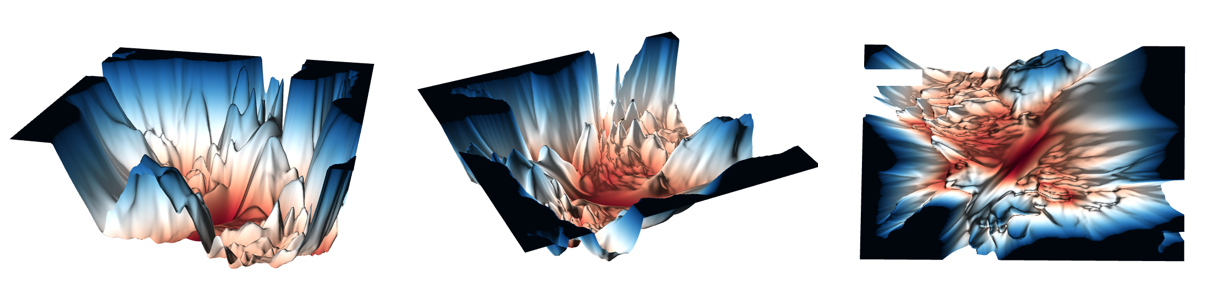
\includegraphics[width=\textwidth]{figures/0intro/intro_landscape.png}
    \caption{A visualisation of the loss landscape of a ResNet-56 model for image classification.}
    \label{fig:high_dim_resnet}
\end{figure}

A saddle point is where among some dimensions, the second-order derivative of the objective is negative, but along others, it is positive. First-order methods slow down in saddle points since they perceive it as a flat region and do not have information about the curvature of the surrounding landscape. This hinders their convergence to a good solution. 

Higher-order methods, by incorporating this curvature information, can identify the nature of saddle points and navigate away from them more effectively. Despite this, it becomes computationally infeasible to process higher-order information. This is because to obtain higher-order information, we would require at least $O(N^2)$ space for $N$ parameters. The computational cost of obtaining higher-order information becomes prohibitive as $N$ increases, which is the case given our deep learning setting. As a practical example, a ResNet-50 model has $N = 25 \times 10^6$ parameters. If we consider each parameter to be represented by 16-bits, we would require $1.25 \times 10^{15}$ bytes, or $1.25$ terabytes of memory to store the second-order information. This is in stark contrast to the $25$ million bytes, or $25$ megabytes, required for first-order information.

\section{KryBall: the best of both worlds}
\label{sec:kryball_intro}

The challenge is to therefore develop an optimisation algorithm that is computationally tractable and scalable, like first-order methods, but can also navigate complex loss landscapes, particularly by escaping saddle points, like higher-order methods. In this thesis, we propose a new optimisation algorithm, KryBall, that combines the benefits of first-order and higher-order methods. We summarise our approach below.

\begin{enumerate}
  \item We use a \textit{Krylov subspace} to approximate local curvature information as a low-dimensional subspace via efficient Hessian-vector products (HvPs).
  \item We analyse this subspace to understand the dominant geometric features of the local landscape. 
  \item We compute the \textit{Saddle-Free Newton} (SFN) direction as a result \citep{dauphin2014sfn}.
  \item We combine this with first-order information such as the gradient and momentum in a \textit{trust region} framework that uses a quadratic model approximation of the local landscape to get a combined, final search direction.
  \item We perform the optimisation step with this direction to optimise our objective.
  \item Optionally, we embed KryBall as a hybrid approach with first-order optimisers such as SGD and Adam, allowing it to be cycled through.
\end{enumerate}

KryBall makes more informed steps than pure first-order methods, particularly in regions like saddle points, while remaining computationally tractable for deep learning. To motivate our method, we show an example in \cref{fig:toy_example}, where first-order methods such as Adam and SGD are hindered on a classic 2D horse saddle, but KryBall successfully escapes it quickly in fewer iterations.

\begin{figure}[h]
  \centering
    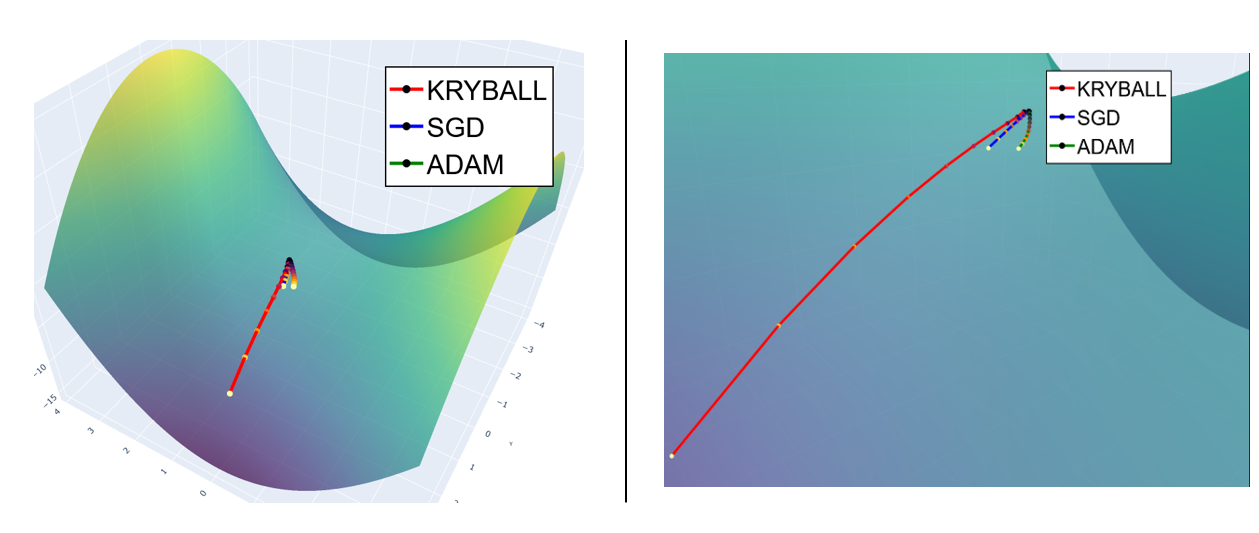
\includegraphics[width=0.85\textwidth]{figures/0intro/intro_toy.png}
    \caption{Left: A classic 2D horse saddle with KryBall, SGD and Adam. Right: A zoomed in version. KryBall successfully escapes the saddle point.}
    \label{fig:toy_example}
\end{figure}

\section{Contributions}
\label{sec:contributions}

Our work focuses on the design and implementation of a novel optimisation algorithm for deep learning, KryBall. In this thesis, we present:
\begin{enumerate}
    \item \textbf{The KryBall Optimisation Algorithm:} The proposal, design, and implementation of KryBall. We combine the benefits of first-order and higher-order methods. KryBall leverages Krylov subspace methods and the SFN direction in a trust-region framework. This enables efficient approximation of local curvature information and navigation of complex loss landscapes, while remaining computationally tractable.
    \item \textbf{Analysis of Loss Landscape Characteristics:} An analysis of the loss landscape properties of common deep learning models and the result of architectural choices (such as activation functions). We investigate the assumptions made when designing an optimiser and the impact of these assumptions on the optimisation process.
    \item \textbf{Extensive Empirical Evaluation:} Experimental validation of KryBall across a range of tasks, such as function optimisation, image classification, and image reconstruction. 
    (\color{red}{can also add the interpretability work here if needs to be more diverse.}\color{black}).
    \item \textbf{A Flexible Experimental Suite:} The development of a modular and configurable software framework for optimiser experiments. This provides a flexible and extensible framework for the implementation, testing, and comparative analysis of various optimisation algorithms. 
    (\color{red}{while not research --- I do think the current framework is a good software suite for a range of tasks that I haven't seen much for optimiser research (except MLPerf). It's quite easy to use, efficient, and extensible. Happy to remove if it doesn't really count as a contribution.}\color{black}).
\end{enumerate}

\section{Thesis outline}
\label{sec:thesis_outline}

To present our contributions, this thesis is organised in the following manner:

\begin{itemize}
    \item \cref{chap:background} provides a mathematical background on optimisation. We formalise the optimisation problem and discuss the geometry of optimisation, including saddle points. This is followed by optimisation in deep learning, where first-order and higher-order methods are explained. We then introduce Krylov subspace methods and trust region algorithms.
    \item \cref{chap:lit_review} provides a comprehensive review of the relevant literature. This includes a survey of first-order and higher-order optimisation algorithms used in deep learning. We compare these methods with our own.
    \item \cref{chap:method} presents the KryBall algorithm. We formally describe its components. This includes the Krylov subspace construction, the SFN computation, and integration with the trust-region framework. We also discuss the assumptions made during the design and outline the hybrid approach.
    \item \cref{chap:results} presents our evaluations. We describe our experimental setup and benchmarking suite. This includes the datasets, model architectures, evaluation metrics, hyperparameter configurations, and comparison with SOTA optimisers. We then present sensitivity analysis and ablation studies.
    \item \cref{chap:discussion} discusses the results. We interpret our findings, analyse potential failure cases and unexpected behaviours, and address current limitations. 
    \item \cref{chap:conclusion} finishes the thesis. We summarise our contributions, discuss the implications of our work, and suggest future work.
\end{itemize}

This chapter has laid the outline for the thesis. We now proceed to \cref{chap:background} to establish the necessary mathematical context.                  % introduction
\chapter{Related Works}
\label{chap:lit_review}

% Categorisation/grouping of the literature
% For each cluster, have a section, covers the major academic works thoroughly
%% Describe, advantages/disadvantages including assumptions, major findings, some analysis
%% Compare to self
% Give the impression that you understand the field thoroughly

Optimisation methods for deep learning have gone through a variety of works that improve the ability to navigate through loss landscapes.
The work in this thesis is heavily inspired by such advances. In this chapter, we explore the major academic works that have played a significant role in the field of optimisation. We provide an overview of key optimisation methods in two main parts: first-order methods and higher-order methods. We also look at other techniques in the field, namely derivative-free optimisation and meta-learning.

\section{First-Order Methods}
In the previous chapter, we saw that the aim of an optimiser is to find $\theta^* = \arg\min_{\theta} F(\theta)$ where $F$ is our objective function to optimise and $\theta$ are the parameters of $F$. First-order methods are characterised under comptuing the first order derivative $\nabla_{\theta}F$ to use in optimisation. We refer to this as $g$, or otherwise $g_t$ if in a stochastic setting.

\subsection{Gradient-Based Methods}
\textbf{Gradient Descent}: One of the earliest methods deployed to solve such optimisation problems is gradient descent (GD), which iteratively updates the parameters with a scalar multiple of the negative gradient direction at each step, $\theta = \theta - \alpha g$. Here, the $\alpha$ parameter is the \textit{learning rate} which controls the step size of each iteration \citep{ruder2016overview}. GD gradually reaches the optimal value of $F$, and given appropriate $\alpha$, reaches the global optimum sub-linearly if $F$ is \textit{convex}, converging linearly if $F$ is \textit{strongly convex} \citep{NoceWrig06}. However, GD is expensive. In many machine learning tasks, $F$ is evaluated with $N$ samples, each with dimensionality $D$ - and so GD requires $O(ND)$ per iteration to evaluate. This becomes infeasible very quickly as $N$ and $D$ scale, and disallows online updates and limits model adaptability \citep{ruder2016overview}. While some parallelisation methods were proposed to combat this, the scalability issue still remains large at hand \citep{alspector1992parallel,NoceWrig06}.

\textbf{Stochastic Gradient Descent}: To address the limitations of GD, stochastic gradient descent (SGD) was proposed. Instead of evaluating $g$ using all $N$, a random sample $n \in N$ is picked and the stochastic gradient $g_t$, which is an unbiased estimate of the real gradient, is computed to update $\theta$ \citep{robbins1951stochastic}. SGD achieves the same convergence rates as GD given $F$ satisfies the same convexity conditions \citep{johnson2013accelerating, nemirovski2009robust}. Each iteration reduces from $O(ND)$ to $O(D)$ given only one sample is used.
This overcomes the disadvantage of GD in two ways: online updates can be performed, and convergence can be accelerated, as an optimal $\theta$ can be found using $n << N$ samples \citep{johnson2013accelerating, nemirovski2009robust}. However, the stochastic gradients used in SGD are inherently noisy and fluctuate. These fluctuations can be beneficial, as they allow SGD to jump from one place to another. This behavior is particularly useful in high-dimensional spaces, where most local minima are approximately equal to the global minimum as the number of parameters increases.

On the other hand, if SGD gets trapped in regions such as saddle points where it is hard to make progress, the fluctuations become less effective. These fluctuations can also lead to large variance in the gradient estimates \citep{sun2019survey}. This can make the optimization process unstable and slow convergence. Convergence is also affected by the learning rate, $\alpha$. Setting a too low $\alpha$ will slow convergence, and setting a too high $\alpha$ can hinder convergence all together, either overshooting or oscillating at the minimum. Choosing a good $\alpha$ usually requires manual tuning, which is arduous and compute heavy.

\textbf{Mini-batch Stochastic Gradient Descent}: The compromise between SGD and GD resulted in mini-batch stochastic gradient descent (mini-batch SGD) \citep{robbins1951stochastic}. mini-batch SGD splits the $N$ samples into $m << N$ i.i.d \textit{batches} (usually ranging from 64 to 256). $\theta$ is updated each iteration by with the stochastic batch gradient based off one batch. Over time, all batches are processed. This reduces the variance in the gradients and makes convergence more stable, which helps optimisation speed, though we note that the $\alpha$ parameter is still needed. mini-batch SGD is now a mainstream technique used for optimising machine learning models. To align with the standard in the literature, we will refer to mini-batch SGD as SGD from now on.

\subsection{Momentum Methods} \label{sec:momentum}
\textbf{Momentum SGD}: Many works have been proposed to improve upon SGD, one of which is momentum (MSGD) \citep{polyak1964some}. The momentum method augments SGD with a \textit{momentum} variable $z$, a decaying average of past gradients controlled by a \textit{momentum factor} $\beta$ \citep{polyak1964some, henriques2019small}. The update is then performed using $z$. 
\begin{align}
    z_{t+1} &= \beta z_{t} - g_t \\
    \theta_{t+1} &= \theta_t + \alpha z_{t+1}
\end{align}
This encourages progress along consistent, but small gradient directions. While this doubles the parameter space needed for updates (since we need $\alpha$ and $\beta$), MSGD yields faster convergence, remains more stable under changing $\alpha$, and is more resistant if $F$ scales poorly \citep{polyak1964some,henriques2019small}. However, this adds another parameter to tune, and the same problems as seen with $\alpha$ arise. Setting a $\beta$ too low won't result in improvements, and setting it too high can result in overshooting.

\textbf{Nesterov Accelerated SGD}: A small improvement over MSGD is Nesterov-Accelerated SGD (NAG). NAG first updates $\theta$ with $z$, and then calculates the gradient based on the updated $\theta$ \citep{nesterov1983method}.
\begin{align}
    \Tilde{\theta}_{t} &= \theta_{t} + \beta z_{t} \\
    z_{t+1} &= \beta z_t - \nabla_{\theta} F(\Tilde{\theta}_{t}) \\
    \theta_{t+1} &= \theta_{t} + \alpha z_{t+1}
\end{align}
Updating based on the future position of $\theta$ includes more gradient information in comparison to traditional momentum, which can provide a better direction \citep{nesterov1983method, dozat2016nadam}. NAG can also result in superlinear convergence when there is no stochasticity \citep{nesterov1983method}.

\subsection{Adaptive Methods}

\textbf{AdaGrad}: To tackle the problem of setting an appropriate $\alpha$, adaptive methods that adjust or scale $\alpha$ directly per parameter were proposed \cite{duchi2011adagrad}. The AdaGrad algorithm keeps a history of previous gradients and adjusts the learning rate dynamically \citep{duchi2011adagrad}. It accumulates the historical gradients via squaring, then scales the current gradient \citep{duchi2011adagrad}. Note that the $\epsilon$ term is added for numerical stability.
\begin{align}
    V_t &= \sqrt{\sum_{i=1}^{t} g_i^2} \\
    \theta_{t+1} &= \theta_{t} + \alpha \frac{g_t}{V_t + \epsilon}
\end{align}
This means only an initial $\alpha$ needs to be set, as during each update the learning rate will adapt due to scaling. Though, as $t \rightarrow \infty$, $V_{t} \rightarrow \infty$, and the learning rate is driven towards zero as the denominator in the update term becomes very large \citep{ruder2016overview,rmsprop2012,zeiler2012adadelta}.
This makes the parameter updates ineffective. This is especially the case in non-convex settings and regions such as saddle points, as the learning rate will be very quickly driven to zero before making sufficient progress.

\textbf{RMSProp and AdaDelta}: To address this, instead of accumulating all of the gradients, RMSProp takes inspiration from momentum \citep{ruder2016overview, rmsprop2012}. It uses an exponential decaying moving average to weight the past squared gradients using a decay parameter $p$ \citep{rmsprop2012, kingma2014adam}.
\begin{align}
    V_t &= \sqrt{p V_{t-1} + (1 - p)g_t^2} 
\end{align}
This simulates having a window size $w$ - where gradients outside of this window are forgotten \citep{rmsprop2012, kingma2014adam}. It priorities more recent gradients and so the learning rate is more stable and doesn't diminish with time. AdaDelta improves upon this and also keeps track of the change in updates, $\Delta(\theta_t)$, performed \citep{zeiler2012adadelta}.
\begin{align}
    U_t = \sqrt{p U_{t-1} + (1 - p)(\Delta(\theta_t))^2}
\end{align}
It uses these accumulative updates at each iteration to perform the actual update which is 
\begin{align}
    \theta_{t+1} = \theta_{t} - \frac{U_{t-1}}{V_{t} + \epsilon} g_t
\end{align}
The key observation here is the absence of $\alpha$. This is a step up from most SGD methods, which require the $\alpha$ parameter. The algorithm is also suitable in non-convex settings since there is no diminishing learning rate \citep{zeiler2012adadelta}. However, the absence of $\alpha$ is replaced with $p$ and $\epsilon$ which still need to be tuned, though these are much less sensitive.

\textbf{Adam}: Perhaps the most successful algorithm for optimisation is Adaptive Moment Estimation (Adam) \citep{kingma2014adam}. Adam maintains two moving averages: one for the gradients themselves, $m_t$, and the same $V_t$ used in RMSProp/AdaDelta \citep{kingma2014adam}. Each of these have an associated decay term $\beta_1$ and $\beta_2$, which weight the gradients and the history \citep{kingma2014adam}.
\begin{align}
m_t &= \beta_1 m_{t-1} + (1 - \beta_1) g_t \label{eq:m_t} \\
V_t &= \sqrt{\beta_2 V_{t-1} + (1 - \beta_2) g_t^2} \\
\hat{m_t} &= \frac{m_t}{1 - (\beta_1)^t} \\
\hat{V_t} &= \frac{V_t}{1 - (\beta_2)^t} \\
\theta_{t+1} &= \theta_t - \alpha \frac{\hat{m_t}}{{\hat{V_t}} + \epsilon} \label{eq:adam_update}
\end{align}
We call $m_t$ and $V_t$ the \textit{first} and \textit{second} moment estimates respectively, with $\beta_1$ and $\beta_2$ being the first and second moment hyper-parameters \citep{kingma2014adam}. Adam has a few key advantages. It uses momentum and exponential decay to smooth out gradients, which makes the optimisation process more stable. It also has bias correction applied to $\hat{m_t}$ and $\hat{V_t}$ to allow for proper initialisation \citep{kingma2014adam}. This ensures they are not biased towards their starting estimates. This is important during early stages of optimisation, as there is insufficient data to estimate the moments. Adam is stable and effective in practice, and works well with both convex and non-convex $F$ - and is the current SOTA optimisation method in deep learning. However, it lacks theoretical guarantees and convergence is not well understood \citep{reddi2019convergence}. Adam has been shown to fail in simple one dimensional convex settings \citep{reddi2019convergence}. It additionally needs two extra parameters, $\beta_1$ and $\beta_2$, in comparison to traditional SGD, which need to be tuned.

\subsection{Adam Variants}
\textbf{AdaMax}: Several variants of Adam have been proposed to address it's limitations. The first variant is AdaMax. AdaMax replaces the $L_2$ norm in $V_t$ with the $L_{\infty}$ norm \citep{kingma2014adam}. Specifically, instead of maintaining the average of the squared gradients $V_t$, AdaMax keeps track of the maximum absolute value of the past gradients \citep{kingma2014adam}.
\begin{align}
    u_t &= \max(\beta_2 \cdot u_{t-1}, |g_t|) \\ 
    \hat{m_t} &= \frac{m_t}{1 - \beta_1^t} \\
    \theta_{t+1} &= \theta_t - \alpha \cdot \frac{\hat{m_t}}{u_t}
\end{align}
Here, the second moment estimate $\hat{V_t}$ is replaced with $u_t$. This is done to make the algorithm more robust, as $u_1, u_2, \dots, u_t$ are influenced by fewer gradients and thus there is less noise. This is especially the case for when the gradients are large and can become numerically unstable \citep{kingma2014adam}. Note that no bias correction is also needed for $u_t$.

\textbf{NAdam}: Another variant of Adam is Nesterov Adam (NAdam), which extends Adam with the NAG method seen in \cref{sec:momentum} \citep{dozat2016nadam}. NAdam uses the NAG update by performing the \textit{Nesterov} trick - in which the previous first moment is replaced with the currently calculated first moment similar to NAG \citep{nesterov1983method,dozat2016nadam}. Condensing the Adam update equations from \cref{eq:m_t} to \cref{eq:adam_update} in \cref{eq:nadam_normal}, the following update is changed from 
\begin{align}
    \theta_{t+1} = \theta_t - \frac{\alpha}{{\hat{V_t}} + \epsilon} (\beta_1 \mathbf{\hat{m}_{t-1}} + \frac{(1 - \beta_1)g_t}{1 - (\beta_1)^t}) \label{eq:nadam_normal}
\end{align}
to 
\begin{align}
    \theta_{t+1} = \theta_t - \frac{\alpha}{{\hat{V_t}} + \epsilon} (\beta_1 \mathbf{\hat{m}_{t}} + \frac{(1 - \beta_1)g_t}{1 - (\beta_1)^t})
\end{align}
Like NAG, NAdam uses the future position of $\theta$ to calculate the gradient and incorporate more information in the update. NAdam has been shown to yield sizeable improvements in performance in comparison to Adam on MNIST and Word2Vec tasks \citep{dozat2016nadam}.

\textbf{AdamW}: Decoupled weight decay regularisation, or AdamW, is a further variant of Adam \citep{loshchilov2017decoupled}. Normally, applying L2 regularisation in Adam involves appending the regularisation term to the gradient update.
\begin{align}
    g_t &= \nabla_{\theta} F(\theta_t) + \lambda \theta_{t-1}
\end{align}
However, upon rescaling, the effect of the regularisation is not properly accounted for and large $g_t$ do not get regularised as much as they should \citep{loshchilov2017decoupled}. To address this, AdamW decouples the weight decay and applies it alongside the update.
\begin{align}
    \theta_{t+1} = \theta_t - \alpha \left( \frac{\hat{m_t}}{\hat{V_t} + \epsilon} + \lambda \theta_t \right)
\end{align}
This is because in adaptive gradient methods, L2 regularisation in the gradient update is \textit{not} the same as weight decay - unlike SGD \citep{loshchilov2017decoupled}. Adam is not effective with L2 regularisation, and so AdamW substantially benefits from this decoupling, improving in performance on CIFAR10 and ImageNet-32 tasks \citep{loshchilov2017decoupled}. AdamW is widely used in practice and is also a current SOTA optimisation method.

\textbf{AMSGrad}: A particularly well-known issue with Adam is it's lack of convergence guarantees. One limitation is that in certain scenarios, Adam aggressively increases the learning rate - even when the algorithm is close to the optimum \citep{reddi2019convergence}. This is because the second moment term $V_t$ can grow indefinitely, and there is a very high dependence on $\beta_2$. For particular $\beta_2$, highly suboptimal solutions can be reached in the case of simple convex settings \citep{reddi2019convergence}.

AMSGrad modifies this by keeping a bound on $\hat{V_t}$ by taking the maximum and using that for it's update rule \citep{reddi2019convergence}.
\begin{align}
    \hat{V_{t}} &= \max(\hat{V}_{t-1}, V_t)
\end{align}
This guarantees that the learning rate is not increased indefinitely, as each $V_t$ is guaranteed to be non decreasing and at least as large as the previous $V_t$'s \citep{reddi2019convergence}. By ensuring this, drastic and aggressive learning rate increases are prevented, and the algorithm convergences better and is more stable. However, AMSGrad is still dependent on $\beta_2$, and cannot show convergence guarantees on any arbitrary $\beta_2$. Some works have demonstrated that problem dependent tuning of $\beta_2$ can lead to convergence, but this still requires manual tuning.

\textbf{ADOPT}: To address the dependency of convergence on $\beta_2$, ADaptive Gradient Method with the OPTimal Convergence Rate (ADOPT) was most recently proposed. ADOPT shows that by modifying the update rules of Adam, convergence can be attained for any $\beta_2 \in [0, 1]$. The non-convergence of Adam can be attributed to the $V_t$ needing to be conditionally independent of the current gradient $g_t$. In a normal Adam update as in \cref{eq:adam_update}, the conditional independence criteria is not satisfied. This is because $\hat{V}_t$ contains information about $g_t$, and so convergence breaks. ADOPT fixes this by modifying the order of the update and the normalisation. Specifically, the normalisation is applied to the current gradient in a modified update rule of $m_t$.
\begin{align}
    m_t = \beta_1 m_{t-1} + (1 - \beta_1) \frac{g_t}{\hat{V}_{t-1} + \epsilon^2}
\end{align}
Here, the previous second moment, $V_{t-1}$ is used to ensure this conditional independence with $g_t$ when scaling and so convergence is guaranteed. In practice, ADOPT uses $\max(\hat{V}_{t-1}, \epsilon)$ instead of $\hat{V}_{t-1} + \epsilon^2$ for the normalisation for performance benefits. The parameter update is shortly applied after.
\begin{align}
    \theta_{t+1} = \theta_{t} - \alpha \cdot m_{t+1}
\end{align}
ADOPT outperforms Adam, AdamW, and AMSGrad on MNIST and CIFAR10 image classification tasks.
It achieves substantial improvements in LLM pretraining and finetuning tasks over Adam and it's aforementioned variants as well. 

\section{Higher-Order Methods}
First-order methods are effective for many optimisation problems for being simple, yet efficient. However, they fall short when encountering ill-conditioned or non-linear objective functions, and flat regions and saddle points. Higher-order methods address these issues by making use of additional curvature information. They find or approximate at least the second-order derivative, $\nabla_{\theta}^{2}F$. For brevity, we will refer to this as $H$, or $H_t$ if used stochastically. 

\subsection{Newton Methods} \label{sec:newton_methods}
\textbf{The Newton Method}: Newton's method is the simplest way to incorporate curvature information. It approximates $F$ by using a second-order Taylor expansion and updates $\theta$ by computing the search direction $d_t$, to which the solution is the gradient preconditioned with the inverse Hessian. We also note that $\alpha = 1$ usually, and learning rates are optional, but usually unused in the update step.
\begin{align}
    d_t &= H_t^{-1} g_t \\
    \theta_{t+1} &= \theta_t - \alpha d_t
\end{align}
This adjusts the step size for each parameter based on the curvature, which results in a key improvement over first-order methods. Newton steps make large progress in flat regions, and are more conservative in steep directions. The method has quadratic convergence given $F \in C^{2}$, and has strong local convergence properties if initialised near a critical point. Though this solves the slowness problem, it can result in moving in the wrong direction. Given a negative eigenvalue, it moves opposite to the gradient step which increases the error. Since it also moves towards optimal $\theta$ along directions with positive eigenvalue, it becomes attracted to saddle points.
Newton's method is also expensive, required $O(N^2)$ memory to store the Hessian and $O(N^3)$ time to compute the inverse Hessian.

\textbf{Saddle-Free Newton}: To address the saddle point concern, the saddle-free newton (SFN) approach was proposed. The SFN applies the $|\cdot|$ (abs) function onto the Hessian, where the absolute value of each eigenvalue is taken.
\begin{align}
    |H_t| &= V_{t} |\Sigma|^{-1} V_{t}^T \\
    \theta_{t+1} &= \theta_t - |H_t|^{-1} g_t
\end{align}
This allows us to escape saddle points and still keep the advantage of taking large steps in low curvature regions. However, this solution is still infeasible. It has the same memory limitations as the Newton method, and adds extra time given we need to reconstruct the Hessian by applying the abs function. Solutions to this issue involve using subspace optimisation methods, which solves the optimisation problem in a lower dimensional subspace. We will look at these in \Cref{sec:subspace_opt}.

\subsection{Quasi-Newton Methods}
\textbf{BFGS}: The computational infeasibility of Newton methods is tackled with Quasi-Newton methods. These aim to approximate the Hessian instead of computing it directly. The Broyden-Fletcher-Goldfarb-Shanno (BFGS) algorithm generates a sequence of matrices to estimate the Hessian. It iteratively refines the estimate using gradient information and rank-two updates at each iteration. The estimate is always positive-definite. Through experimental testing and analysis, these estimates are quite good. BFGS also has effective self-correcting properties - if an estimate become poor at one iteration, within the next few it will correct itself \citep{NoceWrig06}. BFGS reduces the complexity to $O(N^2)$ for computation time.  

A common variant of BFGS, Limited BFGS (L-BFGS), reduces the memory requirement by storing $k$ vectors instead of retaining the full $n\times n$ approximations.

\textbf{SR1}: The Symmetric Rank-One (SR1) method further tackles the infeasibility problem. It approximates the inverse Hessian using the difference between a history of gradients and positions, while ensuring symmetry in the update. The key advantage of SR1 is that it uses only rank-updates, but also does not guarantee positive definiteness. This makes it beneficial in non-convex settings. Albeit at the cost of stability, it helps the algorithm capture more curvature information.

\textbf{Stochastic Trust Region Methods}: 

\subsection{Diagonal Hessian Estimation} \label{sec:diag_hessian}
\textbf{AdaHessian}: As Quasi-Newton methods aim to estimate the inverse Hessian, improvements have been made to use diagonal hessian estimates as well. AdaHessian modifies the second moment from Adam to use the squared diagonal estimate of the Hessian \citep{yao2021adahessian}.
\begin{align}
    \hat{D}_t &\approx \text{diag}(H_t) \\
    V_t &= \sqrt{\beta_2 V_{t-1} + (1 - \beta_2) \hat{D}_t\hat{D}_t}
\end{align}
This brings down the space complexity to $O(D)$, and makes it more feasible to use incorporate second order information \citep{yao2021adahessian}. Though, as a trade-off, an extra backward pass is required per iteration. AdaHessian performs well in image classification, NLP, and recommender system tasks \citep{yao2021adahessian}.

\textbf{Sophia} : A more effective approach to using diagonal estimates was proposed by Second-order Clipped Stochastic Optimisation (Sophia). Sophia uses a diagonal estimate of the Hessian as a preconditioner to the first moment in it's update alongside a clipping mechanism. This was motivated by heterogenous curvature in deep learning models, in which traditional optimisers struggle with. 

Sophia first computes the diagonal estimate of the Hessian, $\bar{D}_t$, every $k$ iterations using either the Hutchinson or Gauss-Newton-Bartlett estimation methods via an estimator $E$. 
\begin{align}
    \hat{D}_t &= E(\theta_t) \quad E \in \{\text{Hutchinson, Gauss-Newton-Bartlett} \} \\
    \bar{D}_t &= 
    \begin{cases}
        \beta_2 \bar{D}_{t-k} + (1 - \beta_2) \hat{D}_t & \text{if } t \mod k = 1, \\
        \bar{D}_{t-1} & \text{otherwise}
    \end{cases}
\end{align}
This is then put into a clipping function that controls the worst case size update, in which the update rule is
\begin{align}
    \theta_{t+1} = \theta_t - \alpha \cdot \text{clip}(\frac{m_t}{\max(\gamma \cdot \bar{D}_t, \epsilon)}, \rho)
\end{align}
where $\text{clip}(z, p) = \max(\min(z, p), -p)$ and $\gamma$, $\rho$ are hyper-parameters that function as a scaling factor and a clipping threshold respectively. As mentioned in \cref{sec:newton_methods}, incorporating second order information can result in moving in the wrong direction. To counter this, Sophia considers only the positive entries of $\bar{D}_t$ and clips each coordinate to a maximum step size of $p$ (where $p = 1$ usually). If any entry of $\bar{D}_t$ is negative, Sophia falls back to momentum signSGD - in which the update is scaled by the sign of the gradient for each component, ignoring the magnitude. This ensures that in the worst case, the update is controlled with a size of $p$, improving stability. On language modelling tasks, Sophia converges quicker and achieves better performance in comparison to AdamW.

\subsection{HvP-based Methods}
\textbf{Hessian-Free Optimisation}: Incorporating second order information can be done without explicitly computing the Hessian or it's approximations. Hessian-free optimisation (HF) aims to do this by directly computing \textit{Hessian-vector products} (HvP). Similar to Newton's method, a search direction is computed by solving the following linear system, where $\alpha_t$ is a step size computed to guarantee sufficient decrease.
\begin{align}
    H_t d_t &= - g_t \\ \label{hf:lin_sys}
    \theta_{t+1} &= \theta_t - \alpha_t d_t
\end{align}
The system is solved with the conjugate-gradient solver (CG), an iterative method that solves linear systems. This computes the HvP without using the Hessian, which reduces the space to $O(N)$ and results in $O(KN)$ time, where $K << N$ controls the number of iterations used for CG. However, the CG solver can be very unstable when $H_t$ isn't positive definite. Thus, it breaks down when dealing with noise and stochastically. Ill-conditioned and non-convex problems also add to these issues.

\textbf{CurveBall}: Combining fast HvP's and curvature information with the heavy-ball framework was introduced with CurveBall, hence it's name. CurveBall uses a quadratic approximation around $F$ like the Newton method, and solves the optimisation problem by solving the same linear system as in \cref{hf:lin_sys}. Instead of using CG or matrix inversion, it uses GD to optimise on $d_t$ and finds $\Delta d_t$. 
\begin{align}
\Delta d_{t+1} &= H_t d_t + g_t \\
z_{t+1} &= \beta z_{t} - \alpha_2 \Delta d_{t+1} \\
\theta_{t+1} &\leftarrow \theta_t + \alpha_1 z_{t+1}
\end{align}
The advantage to this is that there is no restriction on $H$. The algorithm can work in non-convex and ill-conditioned problems too, as demonstrated by it's performance on Rosenbrock and the Rahimi-Recht function. The $\Delta d_{t}$ variable keeps track of how $H_t$ and $g_t$ change as $\theta$ evolves, which incorporates the curvature. To amortize cost, it interleaves updates between $\theta$ and $\Delta d_{t+1}$. With the use of fast HvP's through forward-mode (FMAD) and backward-mode automatic differentiation (RMAD), it requires only two passes of back-propagation. This makes it highly efficient and scalable, in which it demonstrates better performance on MNIST and CIFAR10 classification tasks.  

\subsection{Subspace Optimisation Methods}\label{sec:subspace_opt}

\textbf{Krylov Subspace Descent}: Approximate solutions to optimisation problems in low dimensional subspaces are also a popular strategy to involve curvature information. Krylov Subspace Descent (KSD) constructs a basis of vectors $\mathcal{K}_m$ and then finds a search direction in $\mathcal{K}_m$ using BFGS. The Krylov basis is constructed with diagonal Hessian estimate preconditioning.
\begin{align}
    \mathcal{K}_m = \{(D^{-1}H)^{k}D^{-1}g | \quad 0 \leq k \leq m \}
\end{align}
During optimisation, this subspace is converted into a new non-orthogonal subspace $\hat{\mathcal{K}_m}$, where BFGS is run to find to ${\hat{K}v}$ as the search direction, where $\hat{K} \in \hat{\mathcal{K}_m}$. KSD exhibits lower training error and faster running time in comparison to HF on classification tasks such as MNIST and CURVES. It also has no assumptions on $H$, unlike HF which has stability issues if $H$ is not positive semidefinite. We note that the SFN method was initially done with KSD. 

\section{Derivative-Free Optimisation}
For some problems, there may be conditions on $F$ such that $F \notin C^1$, or $g$ is intractable to calculate. Whilst there exist approximations for $g$, derivative-free optimisation aims to find optimal $\theta$ without it.

\textbf{Coordinate Descent}: Coordinate Descent (CD) aims to perform one dimensional search across along each axis direction of $\theta$, till all directions are chosen properly to find optimal $\theta$. Naively, a set of bases $E = \{e_1, ..., e_D \}$ are chosen where $D = \dim(\theta)$. The parameter space is broken down into individual dimensions or coordinates, and optimization proceeds along each direction sequentially. As such, the update at the $j$th dimension is given by
\begin{align}
\theta^{t+1}_j = \arg\min_{\theta_j \in \mathbb{R}} F(\theta^{t+1}_1, \dots, \theta^{t+1}_{j-1}, \theta_j, \theta^t_{j+1}, \dots, \theta^t_D).
\end{align}
This guarantees convergence, as $F$ is set to decrease or stay the same at each iteration, and the convergence of CD is similar to that of GD. The main difference to GD is that each update is always axis aligned, whereas the $g$ in GD may not be aligned with any $e \in E$. Given the algorithm focuses on one dimension at a time, the update is simple, even for complex problems. It is useful for in settings where there is low $D$ or sparse structures. While highly impractical for deep learning settings, as $D$ is high and we do not know of sparsity structures, setting a coordinate basis may be beneficial to accelerate convergence. In optimisers such as Adam that are adaptive to each parameter, we see similarities as both focus on updating each dimension independently, albeit the way they do so are different. 


\section{Meta-Learning Discovery}
A new way to solve optimisation problems is to consider abstracting away the problem. Meta-learning discovery aim to formulate algorithm search such that optimisation methods are found as a result.

\textbf{Lion}: Evo\textbf{L}ved S\textbf{i}gn M\textbf{o}me\textbf{n}tum (Lion) was discovered via a meta-learning approach. It uses momentum and the sign operation to update parameters. The update is as follows:
\begin{align}
    \text{update} &= \text{sign}(\beta_1 m_{t-1} + (1 - \beta_1)g_t) \\ 
    \theta_{t+1} &= \theta_t - \alpha \cdot \text{update} \\ 
    m_t &= \beta_2 m_{t-1} + (1 - \beta_2)g_t
\end{align}
Unlike adaptive methods, there is no second moment $V_t$, and so no normalisation on the first moment is performed. Thus, Lion contributes a fixed size update to $\theta$ at each iteration, only scaling by the output of the $\text{sign}$ function. This is similar to signSGD, mentioned in \cref{sec:diag_hessian} under Sophia. Lion is advantageous given that it is simple and only tracks the momentum. This halves the memory requirement, making it more efficient. Lion gains up to a 2.3x speedup on AdamW. It outperforms AdamW on image classification, vision-language contrastive learning, diffusion modelling and language modelling and pre-training tasks. However, we note that this is the case only on transformer models that Lion is very effective. Further evaluations proving Lion's effectiveness on non-transformer based models are needed to confirm it's effectiveness.




                   % related work
% \chapter{Technical Background}\label{chap:background}

This section should explain all the technical background that is important for being able to read your report. Recall that your report must be completely self-contained, so you should only assume ``mathematical understanding'', but no specific knowledge. All such knowledge should be provided here, e.g., the formalization and vocabulary of the research areas in which your work resides.

Note that this is not the same as reviewing related work. Related work puts the work done/described in your report into context of other (mostly recent) work that's done by others. In contrast the current chapter is not so much about what work others have done, and more about the formalization (and possibly standard techniques) that you require to describe your contributions (but since you probably didn't come up with these formalizations, you of course still need to cite the respective authors).

Please make use of sections and subsections as it's reasonable to better structure this (or any) chapter.
                    % background/framework
% \chapter{Reasonable Title for Main Content}
\label{chap:content}

% Standard structure:
% Formal task description + notation
% Relevant technical background
%% Can refer back to your technical background \Cref{sec:bkg_nerf}.
% Main technical concept
% Architectural details: how the above fits into the network
% Training details

% Words need to go here, two sentences!

% \section{Section heading}
% \label{sec:first_section}

% Also text goes here.

% \subsection{Subsection heading}
% \label{sec:thisone}

% \paragraph{Implementation details. }
% Sentence starts here.

% Replace template text! So many people leave Pascal's words in their final thesis...

% Tables: 
%% See example below
%% tabularx, no vertical lines, toprule, midrule after headings, bottomrule

\begin{table}[!t] % !
\centering
\caption{Ablation study. Meaningful detailed caption full stop. What does the table show? Explain it to me. Who can tell me what a baseline is? Best results are denoted in bold, second-best results are underlined.}
\label{tab:label_here}
\begin{tabularx}{\linewidth}{@{}lCC@{}} % !
\toprule % !
Method & Your Metric $\uparrow$ & Your Other Metric $\downarrow$\\
\midrule % !
Baseline-Random & 3.2 & 12.1 \\
Method A \citep{Oetiker2021LatexIntroduction} & 21.2 & 10.3 \\
Method B \citep{Smith2021Wubalubadubdub} & \underline{21.7} & \textbf{9.8}\\
\midrule % !
Ours & \textbf{22.8} & \underline{9.9}\\
\bottomrule% !
\end{tabularx}
\end{table}

We show in \Cref{tab:label_here} that\dots
Always refer to your tables and figures in the text.

\begin{figure}[!t]
  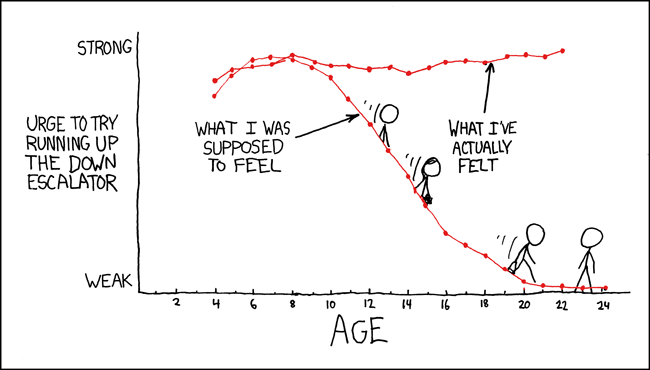
\includegraphics[width=0.5\linewidth]{figures/escalators.png}
  \caption[Short caption for the index]{A detailed meaningful caption. Longer than you would want in your index.}
  \label{fig:your_label}
\end{figure}%
We show in \Cref{fig:your_label} that\dots

% Subcaption for multiple figures in a grid
An example of a $1\times 2$ subfigure on a $1\times 3$ subfigure is given in \Cref{fig:subfig}. You can also refer to subfigures like \Cref{fig:sub_label_a} or just the sub-label \subref{fig:sub_label_a}. This is also an example of using PGFPlot in your thesis, which builds on top of Tikz (draw with vector graphics within latex).

\begin{figure}[!t]\centering
    \begin{subfigure}[]{0.5\linewidth}\centering % this part takes up 50% of the line
        % qpn_pdf_comparison.tex
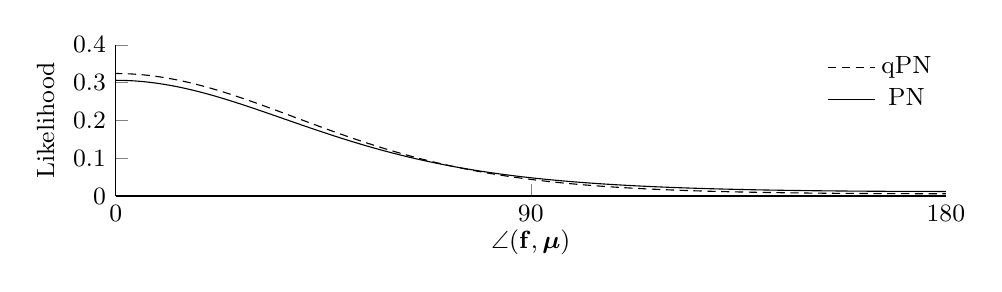
\begin{tikzpicture}
\begin{axis}[
width=\textwidth,
height=3.5cm,
%xmin=-180,
xmin=0,
xmax=180,
xtick={-180, -90, 0, 90, 180},
%xlabel={$\angle(\bbf, \bmu)$ (\textsuperscript{$\circ$})},
xlabel={$\angle(\bbf, \bmu) \vphantom{\rho}$},
xlabel shift=-4pt,
ymin=0,
ymax=0.4,
ytick={0, 0.1,0.2,0.3,0.4},
%ylabel={Relative Likelihood},
ylabel={Likelihood},
%ylabel shift = 1 pt
axis x line*=bottom,
axis y line*=left,
%ymajorticks=false,
%ylabel near ticks,
%hide y axis,
legend entries={qPN,PN},
legend style={draw=none, at={(1,1)}, anchor=north east},
%legend pos=north east,
]

%\addplot [only marks, mark size=2.5pt, mark=*, mark options={solid, black}]
%table[row sep=\\]{
%1 10\\
%};

% vMF for rho = 1
\addplot [black, densely dashed] table [row sep=newline]{
-180	0.00593882225388289
-179.099549774887	0.00594028921694383
-178.199099549775	0.00594469191800688
-177.298649324662	0.00595203579548720
-176.398199099550	0.00596232992266134
-175.497748874437	0.00597558702155373
-174.597298649325	0.00599182348239717
-173.696848424212	0.00601105938868620
-172.796398199100	0.00603331854784825
-171.895947973987	0.00605862852756205
-170.995497748874	0.00608702069775855
-170.095047523762	0.00611853027834409
-169.194597298649	0.00615319639269101
-168.294147073537	0.00619106212694495
-167.393696848424	0.00623217459520314
-166.493246623312	0.00627658501062192
-165.592796398199	0.00632434876251575
-164.692346173087	0.00637552549951384
-163.791895947974	0.00643017921884367
-162.891445722861	0.00648837836181406
-161.990995497749	0.00655019591557253
-161.090545272636	0.00661570952121452
-160.190095047524	0.00668500158832337
-159.289644822411	0.00675815941602121
-158.389194597299	0.00683527532061170
-157.488744372186	0.00691644676989561
-156.588294147074	0.00700177652423943
-155.687843921961	0.00709137278447597
-154.787393696848	0.00718534934671393
-153.886943471736	0.00728382576413018
-152.986493246623	0.00738692751581490
-152.086043021511	0.00749478618273469
-151.185592796398	0.00760753963087304
-150.285142571286	0.00772533220160043
-149.384692346173	0.00784831490931819
-148.484242121061	0.00797664564641068
-147.583791895948	0.00811048939552963
-146.683341670835	0.00825001844922190
-145.782891445723	0.00839541263689825
-144.882441220610	0.00854685955912501
-143.981990995498	0.00870455482920320
-143.081540770385	0.00886870232198060
-142.181090545273	0.00903951442982089
-141.280640320160	0.00921721232563079
-140.380190095048	0.00940202623282070
-139.479739869935	0.00959419570204657
-138.579289644822	0.00979396989455021
-137.678839419710	0.0100016078718829
-136.778389194597	0.0102173788917613
-135.877938969485	0.0104415627097664
-134.977488744372	0.0106744498865556
-134.077038519260	0.0109163421002126
-133.176588294147	0.0111675524633138
-132.276138069035	0.0114284058442382
-131.375687843922	0.0116992391921942
-130.475237618809	0.0119804018653788
-129.574787393697	0.0122722559616246
-128.674337168584	0.0125751766508230
-127.773886943472	0.0128895525083474
-126.873436718359	0.0132157858486230
-125.972986493247	0.0135542930579177
-125.072536268134	0.0139055049253465
-124.172086043022	0.0142698669709984
-123.271635817909	0.0146478397700064
-122.371185592796	0.0150398992712908
-121.470735367684	0.0154465371096080
-120.570285142571	0.0158682609094400
-119.669834917459	0.0163055945791553
-118.769384692346	0.0167590785937651
-117.868934467234	0.0172292702644899
-116.968484242121	0.0177167439932367
-116.068034017009	0.0182220915099724
-115.167583791896	0.0187459220908591
-114.267133566783	0.0192888627548955
-113.366683341671	0.0198515584366881
-112.466233116558	0.0204346721328465
-111.565782891446	0.0210388850193775
-110.665332666333	0.0216648965373200
-109.764882441221	0.0223134244437436
-108.864432216108	0.0229852048251019
-107.963981990996	0.0236809920698135
-107.063531765883	0.0244015587968176
-106.163081540770	0.0251476957367373
-105.262631315658	0.0259202115621660
-104.362181090545	0.0267199326634852
-103.461730865433	0.0275477028665194
-102.561280640320	0.0284043830882373
-101.660830415208	0.0292908509266224
-100.760380190095	0.0302080001807604
-99.8599299649825	0.0311567402971212
-98.9594797398700	0.0321379957379657
-98.0590295147574	0.0331527052677639
-97.1585792896448	0.0342018211534897
-96.2581290645323	0.0352863082746524
-95.3576788394197	0.0364071431389349
-94.4572286143072	0.0375653127993466
-93.5567783891946	0.0387618136688487
-92.6563281640820	0.0399976502284956
-91.7558779389695	0.0412738336252365
-90.8554277138569	0.0425913801556567
-89.9549774887444	0.0439513096320993
-89.0545272636318	0.0453546436278014
-88.1540770385193	0.0468024035979032
-87.2536268134067	0.0482956088734487
-86.3531765882942	0.0498352745257916
-85.4527263631816	0.0514224090991508
-84.5522761380690	0.0530580122094313
-83.6518259129565	0.0547430720078351
-82.7513756878439	0.0564785625082354
-81.8509254627314	0.0582654407777803
-80.9504752376188	0.0601046439907230
-80.0500250125063	0.0619970863460492
-79.1495747873937	0.0639436558500913
-78.2491245622811	0.0659452109659746
-77.3486743371686	0.0680025771324419
-76.4482241120560	0.0701165431553428
-75.5477738869435	0.0722878574758518
-74.6473236618309	0.0745172243202989
-73.7468734367184	0.0768052997373481
-72.8464232116058	0.0791526875291440
-71.9459729864932	0.0815599350839663
-71.0455227613807	0.0840275291188753
-70.1450725362682	0.0865558913417989
-69.2446223111556	0.0891453740434987
-68.3441720860430	0.0917962556308582
-67.4437218609305	0.0945087361139464
-66.5432716358179	0.0972829325603250
-65.6428214107053	0.100118874531089
-64.7423711855928	0.103016499514127
-63.8419209604802	0.105975648371097
-62.9414707353677	0.108996060815557
-62.0410205102551	0.112077370940665
-61.1405702851426	0.115219102815727
-60.2401200600300	0.118420666171763
-59.3396698349175	0.121681352197045
-58.4392196098049	0.125000329464289
-57.5387693846923	0.128376640011893
-56.6383191595798	0.131809195602141
-55.7378689344672	0.135296774179841
-54.8374187093547	0.138838016555232
-53.9369684842421	0.142431423335300
-53.0365182591296	0.146075352127816
-52.1360680340170	0.149768015042453
-51.2356178089045	0.153507476513277
-50.3351675837919	0.157291651466663
-49.4347173586793	0.161118303858358
-48.5342671335668	0.164985045602857
-47.6338169084542	0.168889335917619
-46.7333666833417	0.172828481103815
-45.8329164582291	0.176799634784276
-44.9324662331166	0.180799798618193
-44.0320160080040	0.184825823510745
-43.1315657828915	0.188874411334372
-42.2311155577789	0.192942117176725
-41.3306653326663	0.197025352128509
-40.4302151075538	0.201120386622447
-39.5297648824412	0.205223354332458
-38.6293146573287	0.209330256639849
-37.7288644322161	0.213436967670909
-36.8284142071036	0.217539239907724
-35.9279639819910	0.221632710371378
-35.0275137568784	0.225712907373920
-34.1270635317659	0.229775257832610
-33.2266133066533	0.233815095137021
-32.3261630815408	0.237827667556573
-31.4257128564282	0.241808147173025
-30.5252626313157	0.245751639319396
-29.6248124062031	0.249653192503717
-28.7243621810905	0.253507808792959
-27.8239119559780	0.257310454629482
-26.9234617308654	0.261056072049395
-26.0230115057529	0.264739590269345
-25.1225612806403	0.268355937605495
-24.2221110555278	0.271900053685817
-23.3216608304152	0.275366901914323
-22.4212106053026	0.278751482143549
-21.5207603801901	0.282048843509474
-20.6203101550775	0.285254097381142
-19.7198599299650	0.288362430375528
-18.8194097048524	0.291369117386807
-17.9189594797399	0.294269534577931
-17.0185092546273	0.297059172281551
-16.1180590295148	0.299733647756692
-15.2176088044022	0.302288717747257
-14.3171585792896	0.304720290788432
-13.4167083541771	0.307024439207360
-12.5162581290645	0.309197410765067
-11.6158079039520	0.311235639887556
-10.7153576788394	0.313135758435248
-9.81490745372686	0.314894605961522
-8.91445722861431	0.316509239412957
-8.01400700350175	0.317976942226093
-7.11355677838920	0.319295232777978
-6.21310655327664	0.320461872150507
-5.31265632816408	0.321474871171589
-4.41220610305153	0.322332496699389
-3.51175587793897	0.323033277119411
-2.61130565282641	0.323576007027809
-1.71085542771386	0.323959751078206
-0.810405202601301	0.324183846973289
0.0900450225112556	0.324247907586555
0.990495247623812	0.324151822203856
1.89094547273637	0.323895756878645
2.79139569784892	0.323480153899192
3.69184592296148	0.322905730370374
4.59229614807404	0.322173475916992
5.49274637318659	0.321284649519833
6.39319659829915	0.320240775499918
7.29364682341171	0.319043638670494
8.19409704852426	0.317695278680277
9.09454727363682	0.316197983575280
9.99499749874938	0.314554282610218
10.8954477238619	0.312766938343857
11.7958979489745	0.310838938055944
12.6963481740870	0.308773484526241
13.5967983991996	0.306573986218938
14.4972486243122	0.304244046918075
15.3976988494247	0.301787454861779
16.2981490745373	0.299208171424888
17.1985992996498	0.296510319401079
18.0990495247624	0.293698170936778
18.9994997498749	0.290776135170035
19.8999499749875	0.287748745628064
20.8004002001001	0.284620647437413
21.7008504252126	0.281396584400635
22.6013006503252	0.278081385992965
23.5017508754377	0.274679954331800
24.4022011005503	0.271197251170849
25.3026513256628	0.267638284969552
26.2031015507754	0.264008098086887
27.1035517758879	0.260311754146935
28.0040020010005	0.256554325621615
28.9044522261131	0.252740881673818
29.8049024512256	0.248876476301843
30.7053526763382	0.244966136823481
31.6058029014507	0.241014852735445
32.5062531265633	0.237027564981075
33.4067033516758	0.233009155656326
34.3071535767884	0.228964438181105
35.2076038019010	0.224898147960011
36.1080540270135	0.220814933553444
37.0085042521261	0.216719348377025
37.9089544772386	0.212615842944160
38.8094047023512	0.208508757663596
39.7098549274637	0.204402316200782
40.6103051525763	0.200300619408942
41.5107553776888	0.196207639832926
42.4112056028014	0.192127216786127
43.3116558279140	0.188063051998118
44.2121060530265	0.184018705828143
45.1125562781391	0.179997594037169
46.0130065032516	0.176002985108988
46.9134567283642	0.172037998108720
47.8139069534767	0.168105601065130
48.7143571785893	0.164208609861365
49.6148074037019	0.160349687617115
50.5152576288144	0.156531344543698
51.4157078539270	0.152755938252314
52.3161580790395	0.149025674494559
53.2166083041521	0.145342608313332
54.1170585292646	0.141708645581482
55.0175087543772	0.138125544904884
55.9179589794898	0.134594919866156
56.8184092046023	0.131118241584907
57.7188594297149	0.127696841570189
58.6193096548274	0.124331914840811
59.5197598799400	0.121024523289202
60.4202101050525	0.117775599264758
61.3206603301651	0.114585949352893
62.2211105552777	0.111456258326433
63.1215607803902	0.108387093246516
64.0220110055028	0.105378907690763
64.9224612306153	0.102432046087175
65.8229114557279	0.0995467481329287
66.7233616808404	0.0967231532781166
67.6238119059530	0.0939613052552814
68.5242621310655	0.0912611566365539
69.4247123561781	0.0886225734011217
70.3251625812906	0.0860453394967439
71.2256128064032	0.0835291613800178
72.1260630315158	0.0810736725211163
73.0265132566283	0.0786784378597283
73.9269634817409	0.0763429581999501
74.8274137068534	0.0740666745328909
75.7278639319660	0.0718489722767505
76.6283141570786	0.0696891854251139
77.5287643821911	0.0675866005951714
78.4292146073037	0.0655404609685113
79.3296648324162	0.0635499701180427
80.2301150575288	0.0616142957154864
81.1305652826413	0.0597325731147192
82.0310155077539	0.0579039088070629
82.9314657328664	0.0561273837453856
83.8319159579790	0.0544020565346108
84.7323661830915	0.0527269664869240
85.6328164082041	0.0511011365406147
86.5332666333167	0.0495235760421009
87.4337168584292	0.0479932833912480
88.3341670835418	0.0465092485506194
89.2346173086543	0.0450704554197764
90.1350675337669	0.0436758840761902
91.0355177588794	0.0423245128847245
91.9359679839920	0.0410153204780172
92.8364182091046	0.0397472876104059
93.7368684342171	0.0385193988883359
94.6373186593297	0.0373306443804387
95.5377688844422	0.0361800211106878
96.4382191095548	0.0350665344382275
97.3386693346673	0.0339891993276222
98.2391195597799	0.0329470415134061
99.1395697848924	0.0319390985629079
100.040020010005	0.0309644208414048
100.940470235118	0.0300220723837080
101.840920460230	0.0291111316763113
102.741370685343	0.0282306923542451
103.641820910455	0.0273798638167670
104.542271135568	0.0265577717659938
105.442721360680	0.0257635586725385
106.343171585793	0.0249963841721591
107.243621810905	0.0242554253973593
108.144072036018	0.0235398772478007
109.044522261131	0.0228489526032991
109.944972486243	0.0221818824830783
110.845422711356	0.0215379161548540
111.745872936468	0.0209163211972065
112.646323161581	0.0203163835185896
113.546773386693	0.0197374073362014
114.447223611806	0.0191787151178225
115.347673836918	0.0186396474896023
116.248124062031	0.0181195631126486
117.148574287144	0.0176178385311507
118.049024512256	0.0171338679946382
118.949474737369	0.0166670632568543
119.849924962481	0.0162168533535965
120.750375187594	0.0157826843617553
121.650825412706	0.0153640191416623
122.551275637819	0.0149603370647366
123.451725862931	0.0145711337283091
124.352176088044	0.0141959206593846
125.252626313157	0.0138342250089991
126.153076538269	0.0134855892387171
127.053526763382	0.0131495708007177
127.953976988494	0.0128257418128139
128.854427213607	0.0125136887296590
129.754877438719	0.0122130120113005
130.655327663832	0.0119233257901550
131.555777888944	0.0116442575373965
132.456228114057	0.0113754477296674
133.356678339170	0.0111165495169503
134.257128564282	0.0108672283923641
135.157578789395	0.0106271618645816
136.058029014507	0.0103960391335011
136.958479239620	0.0101735607697450
137.858929464732	0.00995943839850056
138.759379689845	0.00975339438816534
139.659829914958	0.00955516154420918
140.560280140070	0.00936448280861884
141.460730365183	0.00918111096524667
142.361180590295	0.00900480835134479
143.261630815408	0.00883534657552832
144.162081040520	0.00867250624237614
145.062531265633	0.00851607668384570
145.962981490745	0.00836585569764833
146.863431715858	0.00822164929270443
147.763881940971	0.00808327144177255
148.664332166083	0.00795054384132413
149.564782391196	0.00782329567871407
150.465232616308	0.00770136340667929
151.365682841421	0.00758459052517991
152.266133066533	0.00747282737058265
153.166583291646	0.00736593091217264
154.067033516758	0.00726376455596731
154.967483741871	0.00716619795579612
155.867933966984	0.00707310683159993
156.768384192096	0.00698437279489645
157.668834417209	0.00689988318135106
158.569284642321	0.00681953089038679
159.469734867434	0.00674321423176262
160.370185092546	0.00667083677904544
161.270635317659	0.00660230722989844
162.171085542771	0.00653753927310657
163.071535767884	0.00647645146225863
163.971985992996	0.00641896709600501
164.872436218109	0.00636501410481030
165.772886443222	0.00631452494412067
166.673336668334	0.00626743649386745
167.573786893447	0.00622368996423001
168.474237118559	0.00618323080758322
169.374687343672	0.00614600863655781
170.275137568784	0.00611197714814487
171.175587793897	0.00608109405377900
172.076038019010	0.00605332101533875
172.976488244122	0.00602862358700687
173.876938469235	0.00600697116293698
174.777388694347	0.00598833693067831
175.677838919460	0.00597269783031428
176.578289144572	0.00596003451927622
177.478739369685	0.00595033134279801
178.379189594797	0.00594357630998300
179.279639819910	0.00593976107545976
180	0.00593882225388289
};

%% PN
\addplot [black] table [row sep=newline]{
-180	0.0119906989306336
-179.099549774887	0.0119924933487507
-178.199099549775	0.0119978781223270
-177.298649324662	0.0120068578108691
-176.398199099550	0.0120194400196602
-175.497748874437	0.0120356354089268
-174.597298649325	0.0120554577066834
-173.696848424212	0.0120789237252725
-172.796398199100	0.0121060533816135
-171.895947973987	0.0121368697211852
-170.995497748874	0.0121713989457638
-170.095047523762	0.0122096704449472
-169.194597298649	0.0122517168314967
-168.294147073537	0.0122975739805326
-167.393696848424	0.0123472810726244
-166.493246623312	0.0124008806408154
-165.592796398199	0.0124584186216331
-164.692346173087	0.0125199444101309
-163.791895947974	0.0125855109190170
-162.891445722861	0.0126551746419258
-161.990995497749	0.0127289957208917
-161.090545272636	0.0128070380180870
-160.190095047524	0.0128893691918895
-159.289644822411	0.0129760607773467
-158.389194597299	0.0130671882711076
-157.488744372186	0.0131628312208932
-156.588294147074	0.0132630733195801
-155.687843921961	0.0133680025039734
-154.787393696848	0.0134777110583450
-153.886943471736	0.0135922957228169
-152.986493246623	0.0137118578066671
-152.086043021511	0.0138365033066380
-151.185592796398	0.0139663430303262
-150.285142571286	0.0141014927247333
-149.384692346173	0.0142420732100540
-148.484242121061	0.0143882105187790
-147.583791895948	0.0145400360401849
-146.683341670835	0.0146976866702847
-145.782891445723	0.0148613049673048
-144.882441220610	0.0150310393127519
-143.981990995498	0.0152070440781300
-143.081540770385	0.0153894797973578
-142.181090545273	0.0155785133449334
-141.280640320160	0.0157743181198836
-140.380190095048	0.0159770742355263
-139.479739869935	0.0161869687150638
-138.579289644822	0.0164041956930150
-137.678839419710	0.0166289566224783
-136.778389194597	0.0168614604882065
-135.877938969485	0.0171019240254559
-134.977488744372	0.0173505719445543
-134.077038519260	0.0176076371611163
-133.176588294147	0.0178733610318069
-132.276138069035	0.0181479935955373
-131.375687843922	0.0184317938199456
-130.475237618809	0.0187250298529901
-129.574787393697	0.0190279792794509
-128.674337168584	0.0193409293821035
-127.773886943472	0.0196641774072886
-126.873436718359	0.0199980308345694
-125.972986493247	0.0203428076501180
-125.072536268134	0.0206988366234338
-124.172086043022	0.0210664575869432
-123.271635817909	0.0214460217179814
-122.371185592796	0.0218378918225958
-121.470735367684	0.0222424426205569
-120.570285142571	0.0226600610308921
-119.669834917459	0.0230911464571939
-118.769384692346	0.0235361110718786
-117.868934467234	0.0239953800984951
-116.968484242121	0.0244693920911020
-116.068034017009	0.0249585992096429
-115.167583791896	0.0254634674901583
-114.267133566783	0.0259844771085773
-113.366683341671	0.0265221226367289
-112.466233116558	0.0270769132891049
-111.565782891446	0.0276493731587966
-110.665332666333	0.0282400414409081
-109.764882441221	0.0288494726416270
-108.864432216108	0.0294782367710057
-107.963981990996	0.0301269195173747
-107.063531765883	0.0307961224011693
-106.163081540770	0.0314864629058132
-105.262631315658	0.0321985745831513
-104.362181090545	0.0329331071307785
-103.461730865433	0.0336907264384522
-102.561280640320	0.0344721146006246
-101.660830415208	0.0352779698919657
-100.760380190095	0.0361090067025907
-99.8599299649825	0.0369659554295389
-98.9594797398700	0.0378495623208916
-98.0590295147574	0.0387605892687499
-97.1585792896448	0.0396998135471348
-96.2581290645323	0.0406680274907127
-95.3576788394197	0.0416660381100942
-94.4572286143072	0.0426946666393070
-93.5567783891946	0.0437547480108987
-92.6563281640820	0.0448471302539957
-91.7558779389695	0.0459726738105186
-90.8554277138569	0.0471322507646448
-89.9549774887444	0.0483267439805150
-89.0545272636318	0.0495570461430989
-88.1540770385193	0.0508240586970770
-87.2536268134067	0.0521286906785591
-86.3531765882942	0.0534718574344416
-85.4527263631816	0.0548544792242272
-84.5522761380690	0.0562774796991667
-83.6518259129565	0.0577417842536665
-82.7513756878439	0.0592483182440138
-81.8509254627314	0.0607980050696284
-80.9504752376188	0.0623917641122447
-80.0500250125063	0.0640305085286670
-79.1495747873937	0.0657151428930373
-78.2491245622811	0.0674465606848951
-77.3486743371686	0.0692256416197082
-76.4482241120560	0.0710532488190156
-75.5477738869435	0.0729302258178402
-74.6473236618309	0.0748573934076153
-73.7468734367184	0.0768355463135238
-72.8464232116058	0.0788654497058654
-71.9459729864932	0.0809478355458653
-71.0455227613807	0.0830833987672009
-70.1450725362682	0.0852727932954634
-69.2446223111556	0.0875166279087852
-68.3441720860430	0.0898154619439534
-67.4437218609305	0.0921698008534908
-66.5432716358179	0.0945800916204203
-65.6428214107053	0.0970467180387348
-64.7423711855928	0.0995699958689617
-63.8419209604802	0.102150167879651
-62.9414707353677	0.104787398787101
-62.0410205102551	0.107481770107189
-61.1405702851426	0.110233274934753
-60.2401200600300	0.113041812667600
-59.3396698349175	0.115907183693877
-58.4392196098049	0.118829084063194
-57.5387693846923	0.121807100163588
-56.6383191595798	0.124840703428048
-55.7378689344672	0.127929245096019
-54.8374187093547	0.131071951056859
-53.9369684842421	0.134267916803817
-53.0365182591296	0.137516102528583
-52.1360680340170	0.140815328387842
-51.2356178089045	0.144164269974586
-50.3351675837919	0.147561454028085
-49.4347173586793	0.151005254417467
-48.5342671335668	0.154493888434676
-47.6338169084542	0.158025413433309
-46.7333666833417	0.161597723850231
-45.8329164582291	0.165208548647185
-44.9324662331166	0.168855449209545
-44.0320160080040	0.172535817739138
-43.1315657828915	0.176246876177505
-42.2311155577789	0.179985675695130
-41.3306653326663	0.183749096781007
-40.4302151075538	0.187533849965474
-39.5297648824412	0.191336477207404
-38.6293146573287	0.195153353974725
-37.7288644322161	0.198980692044767
-36.8284142071036	0.202814543048072
-35.9279639819910	0.206650802776185
-35.0275137568784	0.210485216270395
-34.1270635317659	0.214313383704607
-33.2266133066533	0.218130767071368
-32.3261630815408	0.221932697675633
-31.4257128564282	0.225714384436182
-30.5252626313157	0.229470922989612
-29.6248124062031	0.233197305586701
-28.7243621810905	0.236888431765564
-27.8239119559780	0.240539119780551
-26.9234617308654	0.244144118760249
-26.0230115057529	0.247698121562262
-25.1225612806403	0.251195778286845
-24.2221110555278	0.254631710405784
-23.3216608304152	0.258000525457425
-22.4212106053026	0.261296832253363
-21.5207603801901	0.264515256537099
-20.6203101550775	0.267650457030071
-19.7198599299650	0.270697141795823
-18.8194097048524	0.273650084848816
-17.9189594797399	0.276504142930569
-17.0185092546273	0.279254272372396
-16.1180590295148	0.281895545961159
-15.2176088044022	0.284423169722143
-14.3171585792896	0.286832499531416
-13.4167083541771	0.289119057468932
-12.5162581290645	0.291278547823218
-11.6158079039520	0.293306872658652
-10.7153576788394	0.295200146857297
-9.81490745372686	0.296954712548851
-8.91445722861431	0.298567152844551
-8.01400700350175	0.300034304793906
-7.11355677838920	0.301353271486775
-6.21310655327664	0.302521433227634
-5.31265632816408	0.303536457713867
-4.41220610305153	0.304396309155400
-3.51175587793897	0.305099256279153
-2.61130565282641	0.305643879168329
-1.71085542771386	0.306029074893636
-0.810405202601301	0.306254061900917
0.0900450225112556	0.306318383127454
0.990495247623812	0.306221907827150
1.89094547273637	0.305964832093011
2.79139569784892	0.305547678073595
3.69184592296148	0.304971291888406
4.59229614807404	0.304236840255493
5.49274637318659	0.303345805852625
6.39319659829915	0.302299981441372
7.29364682341171	0.301101462791123
8.19409704852426	0.299752640447376
9.09454727363682	0.298256190395652
9.99499749874938	0.296615063678810
10.8954477238619	0.294832475031592
11.7958979489745	0.292911890601618
12.6963481740870	0.290857014830893
13.5967983991996	0.288671776576093
14.4972486243122	0.286360314549431
15.3976988494247	0.283926962164750
16.2981490745373	0.281376231875679
17.1985992996498	0.278712799094137
18.0990495247624	0.275941485778241
18.9994997498749	0.273067243778772
19.8999499749875	0.270095138032765
20.8004002001001	0.267030329691546
21.7008504252126	0.263878059268716
22.6013006503252	0.260643629891121
23.5017508754377	0.257332390732894
24.4022011005503	0.253949720709172
25.3026513256628	0.250501012502138
26.2031015507754	0.246991656987747
27.1035517758879	0.243427028126757
28.0040020010005	0.239812468378738
28.9044522261131	0.236153274692489
29.8049024512256	0.232454685120866
30.7053526763382	0.228721866102504
31.6058029014507	0.224959900447232
32.5062531265633	0.221173776056372
33.4067033516758	0.217368375403432
34.3071535767884	0.213548465795149
35.2076038019010	0.209718690427359
36.1080540270135	0.205883560244867
37.0085042521261	0.202047446609377
37.9089544772386	0.198214574774610
38.8094047023512	0.194389018163117
39.7098549274637	0.190574693434904
40.6103051525763	0.186775356333922
41.5107553776888	0.182994598294684
42.4112056028014	0.179235843787884
43.3116558279140	0.175502348380736
44.2121060530265	0.171797197485050
45.1125562781391	0.168123305763601
46.0130065032516	0.164483417163314
46.9134567283642	0.160880105542022
47.8139069534767	0.157315775854166
48.7143571785893	0.153792665859714
49.6148074037019	0.150312848319809
50.5152576288144	0.146878233642130
51.4157078539270	0.143490572938805
52.3161580790395	0.140151461459694
53.2166083041521	0.136862342364202
54.1170585292646	0.133624510795262
55.0175087543772	0.130439118219859
55.9179589794898	0.127307177001348
56.8184092046023	0.124229565169881
57.7188594297149	0.121207031358439
58.6193096548274	0.118240199873322
59.5197598799400	0.115329575869312
60.4202101050525	0.112475550601280
61.3206603301651	0.109678406725546
62.2211105552777	0.106938323625934
63.1215607803902	0.104255382741110
64.0220110055028	0.101629572871462
64.9224612306153	0.0990607954454620
65.8229114557279	0.0965488697271070
66.7233616808404	0.0940935379476967
67.6238119059530	0.0916944703468125
68.5242621310655	0.0893512701089511
69.4247123561781	0.0870634781837980
70.3251625812906	0.0848305779796060
71.2256128064032	0.0826519999205657
72.1260630315158	0.0805271258604151
73.0265132566283	0.0784552933458236
73.9269634817409	0.0764357997243074
74.8274137068534	0.0744679060925798
75.7278639319660	0.0725508410823142
76.6283141570786	0.0706838044812976
77.5287643821911	0.0688659706888748
78.4292146073037	0.0670964920054378
79.3296648324162	0.0653745017564913
80.2301150575288	0.0636991172525342
81.1305652826413	0.0620694425866342
82.0310155077539	0.0604845712721466
82.9314657328664	0.0589435887235342
83.8319159579790	0.0574455745836922
84.7323661830915	0.0559896049015723
85.6328164082041	0.0545747541642304
86.5332666333167	0.0532000971877051
87.4337168584292	0.0518647108713675
88.3341670835418	0.0505676758205666
89.2346173086543	0.0493080778425443
90.1350675337669	0.0480850093206959
91.0355177588794	0.0468975704723242
91.9359679839920	0.0457448704950738
92.8364182091046	0.0446260286072388
93.7368684342171	0.0435401749871184
94.6373186593297	0.0424864516165557
95.5377688844422	0.0414640130337261
96.4382191095548	0.0404720270001645
97.3386693346673	0.0395096750869173
98.2391195597799	0.0385761531845954
99.1395697848924	0.0376706719419775
100.040020010005	0.0367924571376785
100.940470235118	0.0359407499892537
101.840920460230	0.0351148074039608
102.741370685343	0.0343139021752434
103.641820910455	0.0335373231288448
104.542271135568	0.0327843752222949
105.442721360680	0.0320543796013528
106.343171585793	0.0313466736168243
107.243621810905	0.0306606108050087
108.144072036018	0.0299955608348703
109.044522261131	0.0293509094248696
109.944972486243	0.0287260582322320
110.845422711356	0.0281204247172808
111.745872936468	0.0275334419853084
112.646323161581	0.0269645586083166
113.546773386693	0.0264132384288159
114.447223611806	0.0258789603477341
115.347673836918	0.0253612180983568
116.248124062031	0.0248595200080942
117.148574287144	0.0243733887497451
118.049024512256	0.0239023610838160
118.949474737369	0.0234459875933402
119.849924962481	0.0230038324125352
120.750375187594	0.0225754729505372
121.650825412706	0.0221604996113556
122.551275637819	0.0217585155110976
123.451725862931	0.0213691361934304
124.352176088044	0.0209919893441646
125.252626313157	0.0206267145057666
126.153076538269	0.0202729627925378
127.053526763382	0.0199303966071268
127.953976988494	0.0195986893589825
128.854427213607	0.0192775251852916
129.754877438719	0.0189665986748924
130.655327663832	0.0186656145956038
131.555777888944	0.0183742876253586
132.456228114057	0.0180923420874891
133.356678339170	0.0178195116904673
134.257128564282	0.0175555392723672
135.157578789395	0.0173001765502783
136.058029014507	0.0170531838748695
136.958479239620	0.0168143299902687
137.858929464732	0.0165833917994001
138.759379689845	0.0163601541348916
139.659829914958	0.0161444095356449
140.560280140070	0.0159359580291380
141.460730365183	0.0157346069195101
142.361180590295	0.0155401705814634
143.261630815408	0.0153524702599989
144.162081040520	0.0151713338759902
145.062531265633	0.0149965958375855
145.962981490745	0.0148280968574177
146.863431715858	0.0146656837755925
147.763881940971	0.0145092093884149
148.664332166083	0.0143585322828070
149.564782391196	0.0142135166763634
150.465232616308	0.0140740322629848
151.365682841421	0.0139399540640257
152.266133066533	0.0138111622848871
153.166583291646	0.0136875421769826
154.067033516758	0.0135689839050041
154.967483741871	0.0134553824194098
155.867933966984	0.0133466373340562
156.768384192096	0.0132426528088973
157.668834417209	0.0131433374376688
158.569284642321	0.0130486041404809
159.469734867434	0.0129583700612387
160.370185092546	0.0128725564698137
161.270635317659	0.0127910886688885
162.171085542771	0.0127138959054001
163.071535767884	0.0126409112865073
163.971985992996	0.0125720717000112
164.872436218109	0.0125073177391591
165.772886443222	0.0124465936317643
166.673336668334	0.0123898471735780
167.573786893447	0.0123370296658506
168.474237118559	0.0122880958570252
169.374687343672	0.0122430038885056
170.275137568784	0.0122017152444478
171.175587793897	0.0121641947055252
172.076038019010	0.0121304103066208
172.976488244122	0.0121003332984059
173.876938469235	0.0120739381127641
174.777388694347	0.0120512023320271
175.677838919460	0.0120321066619893
176.578289144572	0.0120166349086751
177.478739369685	0.0120047739588320
178.379189594797	0.0119965137641322
179.279639819910	0.0119918473290633
180	0.0119906989306336
};

\end{axis}
\end{tikzpicture}
        \vspace{-18pt}
        \caption{Relative likelihood ($\rho = 1$)}
        \label{fig:sub_label_a}
    \end{subfigure}\hfill % any excess horizontal space goes between the subfigures
    \begin{subfigure}[]{0.5\linewidth}\centering
        \begin{tikzpicture}
\begin{axis}[
scaled ticks=false,
tick label style={/pgf/number format/fixed},
width=\textwidth,
height=3.5cm,
xmin=0,
xmax=5,
xtick={0, 1, ..., 5},
xlabel={$\rho \vphantom{\angle(\bbf, \bmu)}$},
xlabel shift=-4pt,
ymin=0,
ymax=0.04,
ytick={0, 0.01, ...,0.04},
ylabel={MAE},
%ylabel shift=-2pt,
axis x line*=bottom,
axis y line*=left,
%ymajorticks=false,
%ylabel near ticks,
%hide y axis,
%legend entries={$\vMF$,$\PN$},
%legend style={draw=none, at={(1,1)}, anchor=north east},
%legend pos=north east,
]

%\addplot [only marks, mark size=2.5pt, mark=*, mark options={solid, black}]
%table[row sep=\\]{
%1 10\\
%};

%% MAE
\addplot [black] table [row sep=newline]{
0.100000000000000	0.0413191281236007
0.200000000000000	0.0346139984696496
0.300000000000000	0.0287655282865310
0.400000000000000	0.0237540068813730
0.500000000000000	0.0195422603081568
0.600000000000000	0.0160829910864740
0.700000000000000	0.0133195988920811
0.800000000000000	0.0111819311945709
0.900000000000000	0.00959030244918633
1	0.00845004251628531
1.10000000000000	0.00766221054548387
1.20000000000000	0.00713263091784733
1.30000000000000	0.00678074719239092
1.40000000000000	0.00654514421515479
1.50000000000000	0.00637890241051719
1.60000000000000	0.00625222568688656
1.70000000000000	0.00614385236628324
1.80000000000000	0.00604225040266751
1.90000000000000	0.00594325703404724
2	0.00584243421372227
2.10000000000000	0.00573946498348980
2.20000000000000	0.00563494957933974
2.30000000000000	0.00552965882016238
2.40000000000000	0.00542408740054571
2.50000000000000	0.00531819228966805
2.60000000000000	0.00521173034184175
2.70000000000000	0.00510893640257420
2.80000000000000	0.00500440880697224
2.90000000000000	0.00490423025006244
3.00000000000000	0.00480464961892366
3.10000000000000	0.00470596094922317
3.20000000000000	0.00460899176414898
3.30000000000000	0.00451506785319796
3.40000000000000	0.00442358842394028
3.50000000000000	0.00433382063316873
3.60000000000000	0.00424710238945909
3.70000000000000	0.00416346872314328
3.80000000000000	0.00408199500296547
3.90000000000000	0.00400204393072496
4	0.00392277575732362
4.10000000000000	0.00384711043735623
4.20000000000000	0.00377563566639987
4.30000000000000	0.00370306328274511
4.40000000000000	0.00363438691018970
4.50000000000000	0.00356863657853114
4.60000000000000	0.00350096684493657
4.70000000000000	0.00344123882469621
4.80000000000000	0.00337624008011355
4.90000000000000	0.00332126663698587
5.00000000000000	0.00326021275980349
5.10000000000000	0.00320831280363775
5.20000000000000	0.00315218952938847
5.30000000000000	0.00310128823298805
5.40000000000000	0.00305087424444898
5.50000000000000	0.00299849472816950
5.60000000000000	0.00295442142273135
5.70000000000000	0.00290599225929935
5.80000000000000	0.00286044892770108
5.90000000000000	0.00281913064321619
6	0.00277412406175830
6.10000000000000	0.00273221253592677
6.20000000000000	0.00269484671225199
6.30000000000000	0.00265427356087413
6.40000000000000	0.00261227041931178
6.50000000000000	0.00257972468941359
6.60000000000000	0.00254431821113954
6.70000000000000	0.00250632851637804
6.80000000000000	0.00247084860356331
6.90000000000000	0.00244116499294787
7	0.00240910028589179
7.10000000000000	0.00237487578991004
7.20000000000000	0.00234078460131801
7.30000000000000	0.00231503276864338
7.40000000000000	0.00228723026026129
7.50000000000000	0.00225755230706364
7.60000000000000	0.00222617117499046
7.70000000000000	0.00219797456116073
7.80000000000000	0.00217507443548226
7.90000000000000	0.00215049223483861
8	0.00212436344258786
8.10000000000000	0.00209682136295644
8.20000000000000	0.00206799676653635
8.30000000000000	0.00204845650327287
8.40000000000000	0.00202794580224906
8.50000000000000	0.00200610148667098
8.60000000000000	0.00198302589451114
8.70000000000000	0.00195881974468721
8.80000000000000	0.00193358190998049
8.90000000000000	0.00191431249473836
9	0.00189725321466546
9.10000000000000	0.00187908073990816
9.20000000000000	0.00185987160506170
9.30000000000000	0.00183970132685681
9.40000000000000	0.00181864425438302
9.50000000000000	0.00179677342856303
9.60000000000000	0.00177741929741420
9.70000000000000	0.00176350894505390
9.80000000000000	0.00174868562616075
9.90000000000000	0.00173300508406668
10	0.00171652245632889
};

\end{axis}
\end{tikzpicture}
        \vspace{-18pt}
        \caption{Mean Absolute Error}
        \label{fig:sub_label_b}
    \end{subfigure}\vfill % This indicates to add a new row
    \begin{subfigure}[]{0.33\linewidth}\centering % this part takes up 50% of the line
        % qpn_pdf_comparison.tex
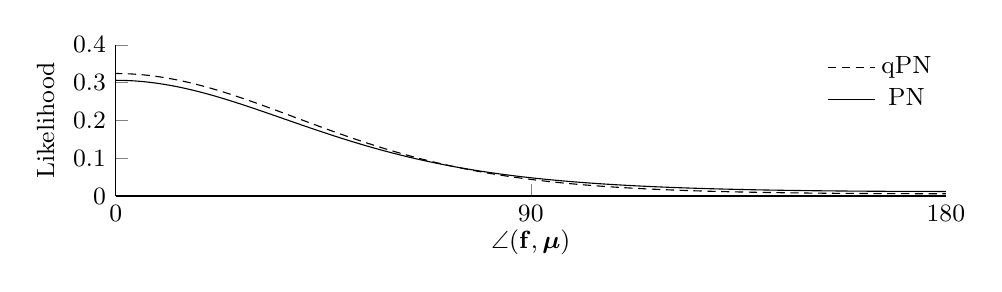
\begin{tikzpicture}
\begin{axis}[
width=\textwidth,
height=3.5cm,
%xmin=-180,
xmin=0,
xmax=180,
xtick={-180, -90, 0, 90, 180},
%xlabel={$\angle(\bbf, \bmu)$ (\textsuperscript{$\circ$})},
xlabel={$\angle(\bbf, \bmu) \vphantom{\rho}$},
xlabel shift=-4pt,
ymin=0,
ymax=0.4,
ytick={0, 0.1,0.2,0.3,0.4},
%ylabel={Relative Likelihood},
ylabel={Likelihood},
%ylabel shift = 1 pt
axis x line*=bottom,
axis y line*=left,
%ymajorticks=false,
%ylabel near ticks,
%hide y axis,
legend entries={qPN,PN},
legend style={draw=none, at={(1,1)}, anchor=north east},
%legend pos=north east,
]

%\addplot [only marks, mark size=2.5pt, mark=*, mark options={solid, black}]
%table[row sep=\\]{
%1 10\\
%};

% vMF for rho = 1
\addplot [black, densely dashed] table [row sep=newline]{
-180	0.00593882225388289
-179.099549774887	0.00594028921694383
-178.199099549775	0.00594469191800688
-177.298649324662	0.00595203579548720
-176.398199099550	0.00596232992266134
-175.497748874437	0.00597558702155373
-174.597298649325	0.00599182348239717
-173.696848424212	0.00601105938868620
-172.796398199100	0.00603331854784825
-171.895947973987	0.00605862852756205
-170.995497748874	0.00608702069775855
-170.095047523762	0.00611853027834409
-169.194597298649	0.00615319639269101
-168.294147073537	0.00619106212694495
-167.393696848424	0.00623217459520314
-166.493246623312	0.00627658501062192
-165.592796398199	0.00632434876251575
-164.692346173087	0.00637552549951384
-163.791895947974	0.00643017921884367
-162.891445722861	0.00648837836181406
-161.990995497749	0.00655019591557253
-161.090545272636	0.00661570952121452
-160.190095047524	0.00668500158832337
-159.289644822411	0.00675815941602121
-158.389194597299	0.00683527532061170
-157.488744372186	0.00691644676989561
-156.588294147074	0.00700177652423943
-155.687843921961	0.00709137278447597
-154.787393696848	0.00718534934671393
-153.886943471736	0.00728382576413018
-152.986493246623	0.00738692751581490
-152.086043021511	0.00749478618273469
-151.185592796398	0.00760753963087304
-150.285142571286	0.00772533220160043
-149.384692346173	0.00784831490931819
-148.484242121061	0.00797664564641068
-147.583791895948	0.00811048939552963
-146.683341670835	0.00825001844922190
-145.782891445723	0.00839541263689825
-144.882441220610	0.00854685955912501
-143.981990995498	0.00870455482920320
-143.081540770385	0.00886870232198060
-142.181090545273	0.00903951442982089
-141.280640320160	0.00921721232563079
-140.380190095048	0.00940202623282070
-139.479739869935	0.00959419570204657
-138.579289644822	0.00979396989455021
-137.678839419710	0.0100016078718829
-136.778389194597	0.0102173788917613
-135.877938969485	0.0104415627097664
-134.977488744372	0.0106744498865556
-134.077038519260	0.0109163421002126
-133.176588294147	0.0111675524633138
-132.276138069035	0.0114284058442382
-131.375687843922	0.0116992391921942
-130.475237618809	0.0119804018653788
-129.574787393697	0.0122722559616246
-128.674337168584	0.0125751766508230
-127.773886943472	0.0128895525083474
-126.873436718359	0.0132157858486230
-125.972986493247	0.0135542930579177
-125.072536268134	0.0139055049253465
-124.172086043022	0.0142698669709984
-123.271635817909	0.0146478397700064
-122.371185592796	0.0150398992712908
-121.470735367684	0.0154465371096080
-120.570285142571	0.0158682609094400
-119.669834917459	0.0163055945791553
-118.769384692346	0.0167590785937651
-117.868934467234	0.0172292702644899
-116.968484242121	0.0177167439932367
-116.068034017009	0.0182220915099724
-115.167583791896	0.0187459220908591
-114.267133566783	0.0192888627548955
-113.366683341671	0.0198515584366881
-112.466233116558	0.0204346721328465
-111.565782891446	0.0210388850193775
-110.665332666333	0.0216648965373200
-109.764882441221	0.0223134244437436
-108.864432216108	0.0229852048251019
-107.963981990996	0.0236809920698135
-107.063531765883	0.0244015587968176
-106.163081540770	0.0251476957367373
-105.262631315658	0.0259202115621660
-104.362181090545	0.0267199326634852
-103.461730865433	0.0275477028665194
-102.561280640320	0.0284043830882373
-101.660830415208	0.0292908509266224
-100.760380190095	0.0302080001807604
-99.8599299649825	0.0311567402971212
-98.9594797398700	0.0321379957379657
-98.0590295147574	0.0331527052677639
-97.1585792896448	0.0342018211534897
-96.2581290645323	0.0352863082746524
-95.3576788394197	0.0364071431389349
-94.4572286143072	0.0375653127993466
-93.5567783891946	0.0387618136688487
-92.6563281640820	0.0399976502284956
-91.7558779389695	0.0412738336252365
-90.8554277138569	0.0425913801556567
-89.9549774887444	0.0439513096320993
-89.0545272636318	0.0453546436278014
-88.1540770385193	0.0468024035979032
-87.2536268134067	0.0482956088734487
-86.3531765882942	0.0498352745257916
-85.4527263631816	0.0514224090991508
-84.5522761380690	0.0530580122094313
-83.6518259129565	0.0547430720078351
-82.7513756878439	0.0564785625082354
-81.8509254627314	0.0582654407777803
-80.9504752376188	0.0601046439907230
-80.0500250125063	0.0619970863460492
-79.1495747873937	0.0639436558500913
-78.2491245622811	0.0659452109659746
-77.3486743371686	0.0680025771324419
-76.4482241120560	0.0701165431553428
-75.5477738869435	0.0722878574758518
-74.6473236618309	0.0745172243202989
-73.7468734367184	0.0768052997373481
-72.8464232116058	0.0791526875291440
-71.9459729864932	0.0815599350839663
-71.0455227613807	0.0840275291188753
-70.1450725362682	0.0865558913417989
-69.2446223111556	0.0891453740434987
-68.3441720860430	0.0917962556308582
-67.4437218609305	0.0945087361139464
-66.5432716358179	0.0972829325603250
-65.6428214107053	0.100118874531089
-64.7423711855928	0.103016499514127
-63.8419209604802	0.105975648371097
-62.9414707353677	0.108996060815557
-62.0410205102551	0.112077370940665
-61.1405702851426	0.115219102815727
-60.2401200600300	0.118420666171763
-59.3396698349175	0.121681352197045
-58.4392196098049	0.125000329464289
-57.5387693846923	0.128376640011893
-56.6383191595798	0.131809195602141
-55.7378689344672	0.135296774179841
-54.8374187093547	0.138838016555232
-53.9369684842421	0.142431423335300
-53.0365182591296	0.146075352127816
-52.1360680340170	0.149768015042453
-51.2356178089045	0.153507476513277
-50.3351675837919	0.157291651466663
-49.4347173586793	0.161118303858358
-48.5342671335668	0.164985045602857
-47.6338169084542	0.168889335917619
-46.7333666833417	0.172828481103815
-45.8329164582291	0.176799634784276
-44.9324662331166	0.180799798618193
-44.0320160080040	0.184825823510745
-43.1315657828915	0.188874411334372
-42.2311155577789	0.192942117176725
-41.3306653326663	0.197025352128509
-40.4302151075538	0.201120386622447
-39.5297648824412	0.205223354332458
-38.6293146573287	0.209330256639849
-37.7288644322161	0.213436967670909
-36.8284142071036	0.217539239907724
-35.9279639819910	0.221632710371378
-35.0275137568784	0.225712907373920
-34.1270635317659	0.229775257832610
-33.2266133066533	0.233815095137021
-32.3261630815408	0.237827667556573
-31.4257128564282	0.241808147173025
-30.5252626313157	0.245751639319396
-29.6248124062031	0.249653192503717
-28.7243621810905	0.253507808792959
-27.8239119559780	0.257310454629482
-26.9234617308654	0.261056072049395
-26.0230115057529	0.264739590269345
-25.1225612806403	0.268355937605495
-24.2221110555278	0.271900053685817
-23.3216608304152	0.275366901914323
-22.4212106053026	0.278751482143549
-21.5207603801901	0.282048843509474
-20.6203101550775	0.285254097381142
-19.7198599299650	0.288362430375528
-18.8194097048524	0.291369117386807
-17.9189594797399	0.294269534577931
-17.0185092546273	0.297059172281551
-16.1180590295148	0.299733647756692
-15.2176088044022	0.302288717747257
-14.3171585792896	0.304720290788432
-13.4167083541771	0.307024439207360
-12.5162581290645	0.309197410765067
-11.6158079039520	0.311235639887556
-10.7153576788394	0.313135758435248
-9.81490745372686	0.314894605961522
-8.91445722861431	0.316509239412957
-8.01400700350175	0.317976942226093
-7.11355677838920	0.319295232777978
-6.21310655327664	0.320461872150507
-5.31265632816408	0.321474871171589
-4.41220610305153	0.322332496699389
-3.51175587793897	0.323033277119411
-2.61130565282641	0.323576007027809
-1.71085542771386	0.323959751078206
-0.810405202601301	0.324183846973289
0.0900450225112556	0.324247907586555
0.990495247623812	0.324151822203856
1.89094547273637	0.323895756878645
2.79139569784892	0.323480153899192
3.69184592296148	0.322905730370374
4.59229614807404	0.322173475916992
5.49274637318659	0.321284649519833
6.39319659829915	0.320240775499918
7.29364682341171	0.319043638670494
8.19409704852426	0.317695278680277
9.09454727363682	0.316197983575280
9.99499749874938	0.314554282610218
10.8954477238619	0.312766938343857
11.7958979489745	0.310838938055944
12.6963481740870	0.308773484526241
13.5967983991996	0.306573986218938
14.4972486243122	0.304244046918075
15.3976988494247	0.301787454861779
16.2981490745373	0.299208171424888
17.1985992996498	0.296510319401079
18.0990495247624	0.293698170936778
18.9994997498749	0.290776135170035
19.8999499749875	0.287748745628064
20.8004002001001	0.284620647437413
21.7008504252126	0.281396584400635
22.6013006503252	0.278081385992965
23.5017508754377	0.274679954331800
24.4022011005503	0.271197251170849
25.3026513256628	0.267638284969552
26.2031015507754	0.264008098086887
27.1035517758879	0.260311754146935
28.0040020010005	0.256554325621615
28.9044522261131	0.252740881673818
29.8049024512256	0.248876476301843
30.7053526763382	0.244966136823481
31.6058029014507	0.241014852735445
32.5062531265633	0.237027564981075
33.4067033516758	0.233009155656326
34.3071535767884	0.228964438181105
35.2076038019010	0.224898147960011
36.1080540270135	0.220814933553444
37.0085042521261	0.216719348377025
37.9089544772386	0.212615842944160
38.8094047023512	0.208508757663596
39.7098549274637	0.204402316200782
40.6103051525763	0.200300619408942
41.5107553776888	0.196207639832926
42.4112056028014	0.192127216786127
43.3116558279140	0.188063051998118
44.2121060530265	0.184018705828143
45.1125562781391	0.179997594037169
46.0130065032516	0.176002985108988
46.9134567283642	0.172037998108720
47.8139069534767	0.168105601065130
48.7143571785893	0.164208609861365
49.6148074037019	0.160349687617115
50.5152576288144	0.156531344543698
51.4157078539270	0.152755938252314
52.3161580790395	0.149025674494559
53.2166083041521	0.145342608313332
54.1170585292646	0.141708645581482
55.0175087543772	0.138125544904884
55.9179589794898	0.134594919866156
56.8184092046023	0.131118241584907
57.7188594297149	0.127696841570189
58.6193096548274	0.124331914840811
59.5197598799400	0.121024523289202
60.4202101050525	0.117775599264758
61.3206603301651	0.114585949352893
62.2211105552777	0.111456258326433
63.1215607803902	0.108387093246516
64.0220110055028	0.105378907690763
64.9224612306153	0.102432046087175
65.8229114557279	0.0995467481329287
66.7233616808404	0.0967231532781166
67.6238119059530	0.0939613052552814
68.5242621310655	0.0912611566365539
69.4247123561781	0.0886225734011217
70.3251625812906	0.0860453394967439
71.2256128064032	0.0835291613800178
72.1260630315158	0.0810736725211163
73.0265132566283	0.0786784378597283
73.9269634817409	0.0763429581999501
74.8274137068534	0.0740666745328909
75.7278639319660	0.0718489722767505
76.6283141570786	0.0696891854251139
77.5287643821911	0.0675866005951714
78.4292146073037	0.0655404609685113
79.3296648324162	0.0635499701180427
80.2301150575288	0.0616142957154864
81.1305652826413	0.0597325731147192
82.0310155077539	0.0579039088070629
82.9314657328664	0.0561273837453856
83.8319159579790	0.0544020565346108
84.7323661830915	0.0527269664869240
85.6328164082041	0.0511011365406147
86.5332666333167	0.0495235760421009
87.4337168584292	0.0479932833912480
88.3341670835418	0.0465092485506194
89.2346173086543	0.0450704554197764
90.1350675337669	0.0436758840761902
91.0355177588794	0.0423245128847245
91.9359679839920	0.0410153204780172
92.8364182091046	0.0397472876104059
93.7368684342171	0.0385193988883359
94.6373186593297	0.0373306443804387
95.5377688844422	0.0361800211106878
96.4382191095548	0.0350665344382275
97.3386693346673	0.0339891993276222
98.2391195597799	0.0329470415134061
99.1395697848924	0.0319390985629079
100.040020010005	0.0309644208414048
100.940470235118	0.0300220723837080
101.840920460230	0.0291111316763113
102.741370685343	0.0282306923542451
103.641820910455	0.0273798638167670
104.542271135568	0.0265577717659938
105.442721360680	0.0257635586725385
106.343171585793	0.0249963841721591
107.243621810905	0.0242554253973593
108.144072036018	0.0235398772478007
109.044522261131	0.0228489526032991
109.944972486243	0.0221818824830783
110.845422711356	0.0215379161548540
111.745872936468	0.0209163211972065
112.646323161581	0.0203163835185896
113.546773386693	0.0197374073362014
114.447223611806	0.0191787151178225
115.347673836918	0.0186396474896023
116.248124062031	0.0181195631126486
117.148574287144	0.0176178385311507
118.049024512256	0.0171338679946382
118.949474737369	0.0166670632568543
119.849924962481	0.0162168533535965
120.750375187594	0.0157826843617553
121.650825412706	0.0153640191416623
122.551275637819	0.0149603370647366
123.451725862931	0.0145711337283091
124.352176088044	0.0141959206593846
125.252626313157	0.0138342250089991
126.153076538269	0.0134855892387171
127.053526763382	0.0131495708007177
127.953976988494	0.0128257418128139
128.854427213607	0.0125136887296590
129.754877438719	0.0122130120113005
130.655327663832	0.0119233257901550
131.555777888944	0.0116442575373965
132.456228114057	0.0113754477296674
133.356678339170	0.0111165495169503
134.257128564282	0.0108672283923641
135.157578789395	0.0106271618645816
136.058029014507	0.0103960391335011
136.958479239620	0.0101735607697450
137.858929464732	0.00995943839850056
138.759379689845	0.00975339438816534
139.659829914958	0.00955516154420918
140.560280140070	0.00936448280861884
141.460730365183	0.00918111096524667
142.361180590295	0.00900480835134479
143.261630815408	0.00883534657552832
144.162081040520	0.00867250624237614
145.062531265633	0.00851607668384570
145.962981490745	0.00836585569764833
146.863431715858	0.00822164929270443
147.763881940971	0.00808327144177255
148.664332166083	0.00795054384132413
149.564782391196	0.00782329567871407
150.465232616308	0.00770136340667929
151.365682841421	0.00758459052517991
152.266133066533	0.00747282737058265
153.166583291646	0.00736593091217264
154.067033516758	0.00726376455596731
154.967483741871	0.00716619795579612
155.867933966984	0.00707310683159993
156.768384192096	0.00698437279489645
157.668834417209	0.00689988318135106
158.569284642321	0.00681953089038679
159.469734867434	0.00674321423176262
160.370185092546	0.00667083677904544
161.270635317659	0.00660230722989844
162.171085542771	0.00653753927310657
163.071535767884	0.00647645146225863
163.971985992996	0.00641896709600501
164.872436218109	0.00636501410481030
165.772886443222	0.00631452494412067
166.673336668334	0.00626743649386745
167.573786893447	0.00622368996423001
168.474237118559	0.00618323080758322
169.374687343672	0.00614600863655781
170.275137568784	0.00611197714814487
171.175587793897	0.00608109405377900
172.076038019010	0.00605332101533875
172.976488244122	0.00602862358700687
173.876938469235	0.00600697116293698
174.777388694347	0.00598833693067831
175.677838919460	0.00597269783031428
176.578289144572	0.00596003451927622
177.478739369685	0.00595033134279801
178.379189594797	0.00594357630998300
179.279639819910	0.00593976107545976
180	0.00593882225388289
};

%% PN
\addplot [black] table [row sep=newline]{
-180	0.0119906989306336
-179.099549774887	0.0119924933487507
-178.199099549775	0.0119978781223270
-177.298649324662	0.0120068578108691
-176.398199099550	0.0120194400196602
-175.497748874437	0.0120356354089268
-174.597298649325	0.0120554577066834
-173.696848424212	0.0120789237252725
-172.796398199100	0.0121060533816135
-171.895947973987	0.0121368697211852
-170.995497748874	0.0121713989457638
-170.095047523762	0.0122096704449472
-169.194597298649	0.0122517168314967
-168.294147073537	0.0122975739805326
-167.393696848424	0.0123472810726244
-166.493246623312	0.0124008806408154
-165.592796398199	0.0124584186216331
-164.692346173087	0.0125199444101309
-163.791895947974	0.0125855109190170
-162.891445722861	0.0126551746419258
-161.990995497749	0.0127289957208917
-161.090545272636	0.0128070380180870
-160.190095047524	0.0128893691918895
-159.289644822411	0.0129760607773467
-158.389194597299	0.0130671882711076
-157.488744372186	0.0131628312208932
-156.588294147074	0.0132630733195801
-155.687843921961	0.0133680025039734
-154.787393696848	0.0134777110583450
-153.886943471736	0.0135922957228169
-152.986493246623	0.0137118578066671
-152.086043021511	0.0138365033066380
-151.185592796398	0.0139663430303262
-150.285142571286	0.0141014927247333
-149.384692346173	0.0142420732100540
-148.484242121061	0.0143882105187790
-147.583791895948	0.0145400360401849
-146.683341670835	0.0146976866702847
-145.782891445723	0.0148613049673048
-144.882441220610	0.0150310393127519
-143.981990995498	0.0152070440781300
-143.081540770385	0.0153894797973578
-142.181090545273	0.0155785133449334
-141.280640320160	0.0157743181198836
-140.380190095048	0.0159770742355263
-139.479739869935	0.0161869687150638
-138.579289644822	0.0164041956930150
-137.678839419710	0.0166289566224783
-136.778389194597	0.0168614604882065
-135.877938969485	0.0171019240254559
-134.977488744372	0.0173505719445543
-134.077038519260	0.0176076371611163
-133.176588294147	0.0178733610318069
-132.276138069035	0.0181479935955373
-131.375687843922	0.0184317938199456
-130.475237618809	0.0187250298529901
-129.574787393697	0.0190279792794509
-128.674337168584	0.0193409293821035
-127.773886943472	0.0196641774072886
-126.873436718359	0.0199980308345694
-125.972986493247	0.0203428076501180
-125.072536268134	0.0206988366234338
-124.172086043022	0.0210664575869432
-123.271635817909	0.0214460217179814
-122.371185592796	0.0218378918225958
-121.470735367684	0.0222424426205569
-120.570285142571	0.0226600610308921
-119.669834917459	0.0230911464571939
-118.769384692346	0.0235361110718786
-117.868934467234	0.0239953800984951
-116.968484242121	0.0244693920911020
-116.068034017009	0.0249585992096429
-115.167583791896	0.0254634674901583
-114.267133566783	0.0259844771085773
-113.366683341671	0.0265221226367289
-112.466233116558	0.0270769132891049
-111.565782891446	0.0276493731587966
-110.665332666333	0.0282400414409081
-109.764882441221	0.0288494726416270
-108.864432216108	0.0294782367710057
-107.963981990996	0.0301269195173747
-107.063531765883	0.0307961224011693
-106.163081540770	0.0314864629058132
-105.262631315658	0.0321985745831513
-104.362181090545	0.0329331071307785
-103.461730865433	0.0336907264384522
-102.561280640320	0.0344721146006246
-101.660830415208	0.0352779698919657
-100.760380190095	0.0361090067025907
-99.8599299649825	0.0369659554295389
-98.9594797398700	0.0378495623208916
-98.0590295147574	0.0387605892687499
-97.1585792896448	0.0396998135471348
-96.2581290645323	0.0406680274907127
-95.3576788394197	0.0416660381100942
-94.4572286143072	0.0426946666393070
-93.5567783891946	0.0437547480108987
-92.6563281640820	0.0448471302539957
-91.7558779389695	0.0459726738105186
-90.8554277138569	0.0471322507646448
-89.9549774887444	0.0483267439805150
-89.0545272636318	0.0495570461430989
-88.1540770385193	0.0508240586970770
-87.2536268134067	0.0521286906785591
-86.3531765882942	0.0534718574344416
-85.4527263631816	0.0548544792242272
-84.5522761380690	0.0562774796991667
-83.6518259129565	0.0577417842536665
-82.7513756878439	0.0592483182440138
-81.8509254627314	0.0607980050696284
-80.9504752376188	0.0623917641122447
-80.0500250125063	0.0640305085286670
-79.1495747873937	0.0657151428930373
-78.2491245622811	0.0674465606848951
-77.3486743371686	0.0692256416197082
-76.4482241120560	0.0710532488190156
-75.5477738869435	0.0729302258178402
-74.6473236618309	0.0748573934076153
-73.7468734367184	0.0768355463135238
-72.8464232116058	0.0788654497058654
-71.9459729864932	0.0809478355458653
-71.0455227613807	0.0830833987672009
-70.1450725362682	0.0852727932954634
-69.2446223111556	0.0875166279087852
-68.3441720860430	0.0898154619439534
-67.4437218609305	0.0921698008534908
-66.5432716358179	0.0945800916204203
-65.6428214107053	0.0970467180387348
-64.7423711855928	0.0995699958689617
-63.8419209604802	0.102150167879651
-62.9414707353677	0.104787398787101
-62.0410205102551	0.107481770107189
-61.1405702851426	0.110233274934753
-60.2401200600300	0.113041812667600
-59.3396698349175	0.115907183693877
-58.4392196098049	0.118829084063194
-57.5387693846923	0.121807100163588
-56.6383191595798	0.124840703428048
-55.7378689344672	0.127929245096019
-54.8374187093547	0.131071951056859
-53.9369684842421	0.134267916803817
-53.0365182591296	0.137516102528583
-52.1360680340170	0.140815328387842
-51.2356178089045	0.144164269974586
-50.3351675837919	0.147561454028085
-49.4347173586793	0.151005254417467
-48.5342671335668	0.154493888434676
-47.6338169084542	0.158025413433309
-46.7333666833417	0.161597723850231
-45.8329164582291	0.165208548647185
-44.9324662331166	0.168855449209545
-44.0320160080040	0.172535817739138
-43.1315657828915	0.176246876177505
-42.2311155577789	0.179985675695130
-41.3306653326663	0.183749096781007
-40.4302151075538	0.187533849965474
-39.5297648824412	0.191336477207404
-38.6293146573287	0.195153353974725
-37.7288644322161	0.198980692044767
-36.8284142071036	0.202814543048072
-35.9279639819910	0.206650802776185
-35.0275137568784	0.210485216270395
-34.1270635317659	0.214313383704607
-33.2266133066533	0.218130767071368
-32.3261630815408	0.221932697675633
-31.4257128564282	0.225714384436182
-30.5252626313157	0.229470922989612
-29.6248124062031	0.233197305586701
-28.7243621810905	0.236888431765564
-27.8239119559780	0.240539119780551
-26.9234617308654	0.244144118760249
-26.0230115057529	0.247698121562262
-25.1225612806403	0.251195778286845
-24.2221110555278	0.254631710405784
-23.3216608304152	0.258000525457425
-22.4212106053026	0.261296832253363
-21.5207603801901	0.264515256537099
-20.6203101550775	0.267650457030071
-19.7198599299650	0.270697141795823
-18.8194097048524	0.273650084848816
-17.9189594797399	0.276504142930569
-17.0185092546273	0.279254272372396
-16.1180590295148	0.281895545961159
-15.2176088044022	0.284423169722143
-14.3171585792896	0.286832499531416
-13.4167083541771	0.289119057468932
-12.5162581290645	0.291278547823218
-11.6158079039520	0.293306872658652
-10.7153576788394	0.295200146857297
-9.81490745372686	0.296954712548851
-8.91445722861431	0.298567152844551
-8.01400700350175	0.300034304793906
-7.11355677838920	0.301353271486775
-6.21310655327664	0.302521433227634
-5.31265632816408	0.303536457713867
-4.41220610305153	0.304396309155400
-3.51175587793897	0.305099256279153
-2.61130565282641	0.305643879168329
-1.71085542771386	0.306029074893636
-0.810405202601301	0.306254061900917
0.0900450225112556	0.306318383127454
0.990495247623812	0.306221907827150
1.89094547273637	0.305964832093011
2.79139569784892	0.305547678073595
3.69184592296148	0.304971291888406
4.59229614807404	0.304236840255493
5.49274637318659	0.303345805852625
6.39319659829915	0.302299981441372
7.29364682341171	0.301101462791123
8.19409704852426	0.299752640447376
9.09454727363682	0.298256190395652
9.99499749874938	0.296615063678810
10.8954477238619	0.294832475031592
11.7958979489745	0.292911890601618
12.6963481740870	0.290857014830893
13.5967983991996	0.288671776576093
14.4972486243122	0.286360314549431
15.3976988494247	0.283926962164750
16.2981490745373	0.281376231875679
17.1985992996498	0.278712799094137
18.0990495247624	0.275941485778241
18.9994997498749	0.273067243778772
19.8999499749875	0.270095138032765
20.8004002001001	0.267030329691546
21.7008504252126	0.263878059268716
22.6013006503252	0.260643629891121
23.5017508754377	0.257332390732894
24.4022011005503	0.253949720709172
25.3026513256628	0.250501012502138
26.2031015507754	0.246991656987747
27.1035517758879	0.243427028126757
28.0040020010005	0.239812468378738
28.9044522261131	0.236153274692489
29.8049024512256	0.232454685120866
30.7053526763382	0.228721866102504
31.6058029014507	0.224959900447232
32.5062531265633	0.221173776056372
33.4067033516758	0.217368375403432
34.3071535767884	0.213548465795149
35.2076038019010	0.209718690427359
36.1080540270135	0.205883560244867
37.0085042521261	0.202047446609377
37.9089544772386	0.198214574774610
38.8094047023512	0.194389018163117
39.7098549274637	0.190574693434904
40.6103051525763	0.186775356333922
41.5107553776888	0.182994598294684
42.4112056028014	0.179235843787884
43.3116558279140	0.175502348380736
44.2121060530265	0.171797197485050
45.1125562781391	0.168123305763601
46.0130065032516	0.164483417163314
46.9134567283642	0.160880105542022
47.8139069534767	0.157315775854166
48.7143571785893	0.153792665859714
49.6148074037019	0.150312848319809
50.5152576288144	0.146878233642130
51.4157078539270	0.143490572938805
52.3161580790395	0.140151461459694
53.2166083041521	0.136862342364202
54.1170585292646	0.133624510795262
55.0175087543772	0.130439118219859
55.9179589794898	0.127307177001348
56.8184092046023	0.124229565169881
57.7188594297149	0.121207031358439
58.6193096548274	0.118240199873322
59.5197598799400	0.115329575869312
60.4202101050525	0.112475550601280
61.3206603301651	0.109678406725546
62.2211105552777	0.106938323625934
63.1215607803902	0.104255382741110
64.0220110055028	0.101629572871462
64.9224612306153	0.0990607954454620
65.8229114557279	0.0965488697271070
66.7233616808404	0.0940935379476967
67.6238119059530	0.0916944703468125
68.5242621310655	0.0893512701089511
69.4247123561781	0.0870634781837980
70.3251625812906	0.0848305779796060
71.2256128064032	0.0826519999205657
72.1260630315158	0.0805271258604151
73.0265132566283	0.0784552933458236
73.9269634817409	0.0764357997243074
74.8274137068534	0.0744679060925798
75.7278639319660	0.0725508410823142
76.6283141570786	0.0706838044812976
77.5287643821911	0.0688659706888748
78.4292146073037	0.0670964920054378
79.3296648324162	0.0653745017564913
80.2301150575288	0.0636991172525342
81.1305652826413	0.0620694425866342
82.0310155077539	0.0604845712721466
82.9314657328664	0.0589435887235342
83.8319159579790	0.0574455745836922
84.7323661830915	0.0559896049015723
85.6328164082041	0.0545747541642304
86.5332666333167	0.0532000971877051
87.4337168584292	0.0518647108713675
88.3341670835418	0.0505676758205666
89.2346173086543	0.0493080778425443
90.1350675337669	0.0480850093206959
91.0355177588794	0.0468975704723242
91.9359679839920	0.0457448704950738
92.8364182091046	0.0446260286072388
93.7368684342171	0.0435401749871184
94.6373186593297	0.0424864516165557
95.5377688844422	0.0414640130337261
96.4382191095548	0.0404720270001645
97.3386693346673	0.0395096750869173
98.2391195597799	0.0385761531845954
99.1395697848924	0.0376706719419775
100.040020010005	0.0367924571376785
100.940470235118	0.0359407499892537
101.840920460230	0.0351148074039608
102.741370685343	0.0343139021752434
103.641820910455	0.0335373231288448
104.542271135568	0.0327843752222949
105.442721360680	0.0320543796013528
106.343171585793	0.0313466736168243
107.243621810905	0.0306606108050087
108.144072036018	0.0299955608348703
109.044522261131	0.0293509094248696
109.944972486243	0.0287260582322320
110.845422711356	0.0281204247172808
111.745872936468	0.0275334419853084
112.646323161581	0.0269645586083166
113.546773386693	0.0264132384288159
114.447223611806	0.0258789603477341
115.347673836918	0.0253612180983568
116.248124062031	0.0248595200080942
117.148574287144	0.0243733887497451
118.049024512256	0.0239023610838160
118.949474737369	0.0234459875933402
119.849924962481	0.0230038324125352
120.750375187594	0.0225754729505372
121.650825412706	0.0221604996113556
122.551275637819	0.0217585155110976
123.451725862931	0.0213691361934304
124.352176088044	0.0209919893441646
125.252626313157	0.0206267145057666
126.153076538269	0.0202729627925378
127.053526763382	0.0199303966071268
127.953976988494	0.0195986893589825
128.854427213607	0.0192775251852916
129.754877438719	0.0189665986748924
130.655327663832	0.0186656145956038
131.555777888944	0.0183742876253586
132.456228114057	0.0180923420874891
133.356678339170	0.0178195116904673
134.257128564282	0.0175555392723672
135.157578789395	0.0173001765502783
136.058029014507	0.0170531838748695
136.958479239620	0.0168143299902687
137.858929464732	0.0165833917994001
138.759379689845	0.0163601541348916
139.659829914958	0.0161444095356449
140.560280140070	0.0159359580291380
141.460730365183	0.0157346069195101
142.361180590295	0.0155401705814634
143.261630815408	0.0153524702599989
144.162081040520	0.0151713338759902
145.062531265633	0.0149965958375855
145.962981490745	0.0148280968574177
146.863431715858	0.0146656837755925
147.763881940971	0.0145092093884149
148.664332166083	0.0143585322828070
149.564782391196	0.0142135166763634
150.465232616308	0.0140740322629848
151.365682841421	0.0139399540640257
152.266133066533	0.0138111622848871
153.166583291646	0.0136875421769826
154.067033516758	0.0135689839050041
154.967483741871	0.0134553824194098
155.867933966984	0.0133466373340562
156.768384192096	0.0132426528088973
157.668834417209	0.0131433374376688
158.569284642321	0.0130486041404809
159.469734867434	0.0129583700612387
160.370185092546	0.0128725564698137
161.270635317659	0.0127910886688885
162.171085542771	0.0127138959054001
163.071535767884	0.0126409112865073
163.971985992996	0.0125720717000112
164.872436218109	0.0125073177391591
165.772886443222	0.0124465936317643
166.673336668334	0.0123898471735780
167.573786893447	0.0123370296658506
168.474237118559	0.0122880958570252
169.374687343672	0.0122430038885056
170.275137568784	0.0122017152444478
171.175587793897	0.0121641947055252
172.076038019010	0.0121304103066208
172.976488244122	0.0121003332984059
173.876938469235	0.0120739381127641
174.777388694347	0.0120512023320271
175.677838919460	0.0120321066619893
176.578289144572	0.0120166349086751
177.478739369685	0.0120047739588320
178.379189594797	0.0119965137641322
179.279639819910	0.0119918473290633
180	0.0119906989306336
};

\end{axis}
\end{tikzpicture}
        \vspace{-18pt}
        \caption{Relative likelihood ($\rho = 1$)}
        \label{fig:sub_label_c}
    \end{subfigure}\hfill % any excess horizontal space goes between the subfigures
    \begin{subfigure}[]{0.33\linewidth}\centering
        \begin{tikzpicture}
\begin{axis}[
scaled ticks=false,
tick label style={/pgf/number format/fixed},
width=\textwidth,
height=3.5cm,
xmin=0,
xmax=5,
xtick={0, 1, ..., 5},
xlabel={$\rho \vphantom{\angle(\bbf, \bmu)}$},
xlabel shift=-4pt,
ymin=0,
ymax=0.04,
ytick={0, 0.01, ...,0.04},
ylabel={MAE},
%ylabel shift=-2pt,
axis x line*=bottom,
axis y line*=left,
%ymajorticks=false,
%ylabel near ticks,
%hide y axis,
%legend entries={$\vMF$,$\PN$},
%legend style={draw=none, at={(1,1)}, anchor=north east},
%legend pos=north east,
]

%\addplot [only marks, mark size=2.5pt, mark=*, mark options={solid, black}]
%table[row sep=\\]{
%1 10\\
%};

%% MAE
\addplot [black] table [row sep=newline]{
0.100000000000000	0.0413191281236007
0.200000000000000	0.0346139984696496
0.300000000000000	0.0287655282865310
0.400000000000000	0.0237540068813730
0.500000000000000	0.0195422603081568
0.600000000000000	0.0160829910864740
0.700000000000000	0.0133195988920811
0.800000000000000	0.0111819311945709
0.900000000000000	0.00959030244918633
1	0.00845004251628531
1.10000000000000	0.00766221054548387
1.20000000000000	0.00713263091784733
1.30000000000000	0.00678074719239092
1.40000000000000	0.00654514421515479
1.50000000000000	0.00637890241051719
1.60000000000000	0.00625222568688656
1.70000000000000	0.00614385236628324
1.80000000000000	0.00604225040266751
1.90000000000000	0.00594325703404724
2	0.00584243421372227
2.10000000000000	0.00573946498348980
2.20000000000000	0.00563494957933974
2.30000000000000	0.00552965882016238
2.40000000000000	0.00542408740054571
2.50000000000000	0.00531819228966805
2.60000000000000	0.00521173034184175
2.70000000000000	0.00510893640257420
2.80000000000000	0.00500440880697224
2.90000000000000	0.00490423025006244
3.00000000000000	0.00480464961892366
3.10000000000000	0.00470596094922317
3.20000000000000	0.00460899176414898
3.30000000000000	0.00451506785319796
3.40000000000000	0.00442358842394028
3.50000000000000	0.00433382063316873
3.60000000000000	0.00424710238945909
3.70000000000000	0.00416346872314328
3.80000000000000	0.00408199500296547
3.90000000000000	0.00400204393072496
4	0.00392277575732362
4.10000000000000	0.00384711043735623
4.20000000000000	0.00377563566639987
4.30000000000000	0.00370306328274511
4.40000000000000	0.00363438691018970
4.50000000000000	0.00356863657853114
4.60000000000000	0.00350096684493657
4.70000000000000	0.00344123882469621
4.80000000000000	0.00337624008011355
4.90000000000000	0.00332126663698587
5.00000000000000	0.00326021275980349
5.10000000000000	0.00320831280363775
5.20000000000000	0.00315218952938847
5.30000000000000	0.00310128823298805
5.40000000000000	0.00305087424444898
5.50000000000000	0.00299849472816950
5.60000000000000	0.00295442142273135
5.70000000000000	0.00290599225929935
5.80000000000000	0.00286044892770108
5.90000000000000	0.00281913064321619
6	0.00277412406175830
6.10000000000000	0.00273221253592677
6.20000000000000	0.00269484671225199
6.30000000000000	0.00265427356087413
6.40000000000000	0.00261227041931178
6.50000000000000	0.00257972468941359
6.60000000000000	0.00254431821113954
6.70000000000000	0.00250632851637804
6.80000000000000	0.00247084860356331
6.90000000000000	0.00244116499294787
7	0.00240910028589179
7.10000000000000	0.00237487578991004
7.20000000000000	0.00234078460131801
7.30000000000000	0.00231503276864338
7.40000000000000	0.00228723026026129
7.50000000000000	0.00225755230706364
7.60000000000000	0.00222617117499046
7.70000000000000	0.00219797456116073
7.80000000000000	0.00217507443548226
7.90000000000000	0.00215049223483861
8	0.00212436344258786
8.10000000000000	0.00209682136295644
8.20000000000000	0.00206799676653635
8.30000000000000	0.00204845650327287
8.40000000000000	0.00202794580224906
8.50000000000000	0.00200610148667098
8.60000000000000	0.00198302589451114
8.70000000000000	0.00195881974468721
8.80000000000000	0.00193358190998049
8.90000000000000	0.00191431249473836
9	0.00189725321466546
9.10000000000000	0.00187908073990816
9.20000000000000	0.00185987160506170
9.30000000000000	0.00183970132685681
9.40000000000000	0.00181864425438302
9.50000000000000	0.00179677342856303
9.60000000000000	0.00177741929741420
9.70000000000000	0.00176350894505390
9.80000000000000	0.00174868562616075
9.90000000000000	0.00173300508406668
10	0.00171652245632889
};

\end{axis}
\end{tikzpicture}
        \vspace{-18pt}
        \caption{Mean Absolute Error}
        \label{fig:sub_label_d}
    \end{subfigure}\hfill
    \begin{subfigure}[]{0.33\linewidth}\centering
        \begin{tikzpicture}
\begin{axis}[
scaled ticks=false,
tick label style={/pgf/number format/fixed},
width=\textwidth,
height=3.5cm,
xmin=0,
xmax=5,
xtick={0, 1, ..., 5},
xlabel={$\rho \vphantom{\angle(\bbf, \bmu)}$},
xlabel shift=-4pt,
ymin=0,
ymax=0.04,
ytick={0, 0.01, ...,0.04},
ylabel={MAE},
%ylabel shift=-2pt,
axis x line*=bottom,
axis y line*=left,
%ymajorticks=false,
%ylabel near ticks,
%hide y axis,
%legend entries={$\vMF$,$\PN$},
%legend style={draw=none, at={(1,1)}, anchor=north east},
%legend pos=north east,
]

%\addplot [only marks, mark size=2.5pt, mark=*, mark options={solid, black}]
%table[row sep=\\]{
%1 10\\
%};

%% MAE
\addplot [black] table [row sep=newline]{
0.100000000000000	0.0413191281236007
0.200000000000000	0.0346139984696496
0.300000000000000	0.0287655282865310
0.400000000000000	0.0237540068813730
0.500000000000000	0.0195422603081568
0.600000000000000	0.0160829910864740
0.700000000000000	0.0133195988920811
0.800000000000000	0.0111819311945709
0.900000000000000	0.00959030244918633
1	0.00845004251628531
1.10000000000000	0.00766221054548387
1.20000000000000	0.00713263091784733
1.30000000000000	0.00678074719239092
1.40000000000000	0.00654514421515479
1.50000000000000	0.00637890241051719
1.60000000000000	0.00625222568688656
1.70000000000000	0.00614385236628324
1.80000000000000	0.00604225040266751
1.90000000000000	0.00594325703404724
2	0.00584243421372227
2.10000000000000	0.00573946498348980
2.20000000000000	0.00563494957933974
2.30000000000000	0.00552965882016238
2.40000000000000	0.00542408740054571
2.50000000000000	0.00531819228966805
2.60000000000000	0.00521173034184175
2.70000000000000	0.00510893640257420
2.80000000000000	0.00500440880697224
2.90000000000000	0.00490423025006244
3.00000000000000	0.00480464961892366
3.10000000000000	0.00470596094922317
3.20000000000000	0.00460899176414898
3.30000000000000	0.00451506785319796
3.40000000000000	0.00442358842394028
3.50000000000000	0.00433382063316873
3.60000000000000	0.00424710238945909
3.70000000000000	0.00416346872314328
3.80000000000000	0.00408199500296547
3.90000000000000	0.00400204393072496
4	0.00392277575732362
4.10000000000000	0.00384711043735623
4.20000000000000	0.00377563566639987
4.30000000000000	0.00370306328274511
4.40000000000000	0.00363438691018970
4.50000000000000	0.00356863657853114
4.60000000000000	0.00350096684493657
4.70000000000000	0.00344123882469621
4.80000000000000	0.00337624008011355
4.90000000000000	0.00332126663698587
5.00000000000000	0.00326021275980349
5.10000000000000	0.00320831280363775
5.20000000000000	0.00315218952938847
5.30000000000000	0.00310128823298805
5.40000000000000	0.00305087424444898
5.50000000000000	0.00299849472816950
5.60000000000000	0.00295442142273135
5.70000000000000	0.00290599225929935
5.80000000000000	0.00286044892770108
5.90000000000000	0.00281913064321619
6	0.00277412406175830
6.10000000000000	0.00273221253592677
6.20000000000000	0.00269484671225199
6.30000000000000	0.00265427356087413
6.40000000000000	0.00261227041931178
6.50000000000000	0.00257972468941359
6.60000000000000	0.00254431821113954
6.70000000000000	0.00250632851637804
6.80000000000000	0.00247084860356331
6.90000000000000	0.00244116499294787
7	0.00240910028589179
7.10000000000000	0.00237487578991004
7.20000000000000	0.00234078460131801
7.30000000000000	0.00231503276864338
7.40000000000000	0.00228723026026129
7.50000000000000	0.00225755230706364
7.60000000000000	0.00222617117499046
7.70000000000000	0.00219797456116073
7.80000000000000	0.00217507443548226
7.90000000000000	0.00215049223483861
8	0.00212436344258786
8.10000000000000	0.00209682136295644
8.20000000000000	0.00206799676653635
8.30000000000000	0.00204845650327287
8.40000000000000	0.00202794580224906
8.50000000000000	0.00200610148667098
8.60000000000000	0.00198302589451114
8.70000000000000	0.00195881974468721
8.80000000000000	0.00193358190998049
8.90000000000000	0.00191431249473836
9	0.00189725321466546
9.10000000000000	0.00187908073990816
9.20000000000000	0.00185987160506170
9.30000000000000	0.00183970132685681
9.40000000000000	0.00181864425438302
9.50000000000000	0.00179677342856303
9.60000000000000	0.00177741929741420
9.70000000000000	0.00176350894505390
9.80000000000000	0.00174868562616075
9.90000000000000	0.00173300508406668
10	0.00171652245632889
};

\end{axis}
\end{tikzpicture}
        \vspace{-18pt}
        \caption{Mean Absolute Error}
        \label{fig:sub_label_e}
    \end{subfigure}%
    \caption{Main caption here. \subref{fig:sub_label_a} A nice plot in Tikz. \subref{fig:sub_label_b} Also something. \subref{fig:sub_label_c} Ground truth. \subref{fig:sub_label_d} ???? \subref{fig:sub_label_e} !!!!}
    \label{fig:subfig}
\end{figure}

% tikz: high quality vector graphics (diagrams) including in 3D; pgfplots: graphs and data management

% Mathematics:
Inline symbols like this $\Gamma = 0.01$. The flow rate is given by
\begin{equation}
    r = 2VP,
    \label{eq:flowrate}
\end{equation}
where the volume is denoted by $V$ and blah. As shown in \Cref{eq:flowrate}, we see\dots
The other equation environment is this one
\begin{align}
    E &= mc^2\\
      &= m(1-p)\\
      &\rightarrow \sum_{i=1}^{N} w_i \hat{x},
\end{align}
where\dots
$\bv \in \reals^n$ and the loss $\cL_\text{heatmap}$.
Can declare math operators in the macros.
\begin{equation}
    x =
    \begin{cases}
        1 \text{ if bingo,}\\
        2 \text{ otherwise.}
    \end{cases}
\end{equation}

% Referencing:
% Sentence should make sense if you delete the parts inside the parentheses
% Google Scholar
% Use official details rather than arxiv version where possible
% @inproceedings for conferences
% @article for journal articles
% @misc for websites
% ANU library has details on how to do these
For example, these people \citep{engelhardt2024shinobi,Cooper2015SuperfluidVacuumTheory,Oetiker2021LatexIntroduction}.
\citet{Cooper2015SuperfluidVacuumTheory} believe\dots
The trial is stacked \citep{Cooper2015SuperfluidVacuumTheory}.

% References (non-bibliographic):
\Cref{chap:background}
\Cref{eq:flowrate}
\Cref{fig:pageBorders}

% Lists:
\begin{enumerate}
    \item ordered elements
    \item like this
\end{enumerate}
\begin{itemize}
    \item unordered elements
    \item like this
\end{itemize}

% Misc:
% Formal language: no contractions, no idioms
% Clear communication is the goal: precise, concrete examples, reference everything
% First person or passive
% spell-check
% no random capitalisation, only proper nouns or at sentence start
% do not over-use bold or italics
% macros: see macro.tex -- define your own and use them
Smith \etal believe X \citep{Smith2021Wubalubadubdub}.
Jelly, \eg, aeroplane, is good.
Jelly, \ie, aeroplane, is good.
% quotation marks
``Quote here''. % note the ``
% -,--,---
Compound words get hyphens like self-attention. Those hard-to-reach locations.
En dashes are used for ranges like 2--5, and if you have two complete words that you are joining, like Navier--Stokes Theorem or 2D--3D projection.
Em dashes are for emphatic subclauses---like this one---in the middle of a sentence.

% Advice:
%% How to start? Write down all section titles, then subsections, then add a few dot points about what you want to say in each, then fill them out
%% Put in placeholder (empty) figures and tables with a note in the caption saying what you want to be there.
%% Use latex comments (like this) to structure your thoughts. E.g.,

% Task:
This thesis considers the task of\dots
%
% Motivation:
This is a key component of many driver safety systems and so any efficiency improvements have real-world implications.
% Challenges:
However, it's a pain.

This chapter holds your contributions. Depending on your exact topic, you might use only a single chapter for your actual contributions, or several. Even having several is not unusual. Discuss your proposal with your supervisor(s) and propose descriptive titles. 

The following sections give additional advice that is specifically tailored to students who are new to either \LaTeX{} or scientific writing. I \emph{strongly} suggest that you read the entire document carefully! Also use it as checklist after you started writing and after finishing.


\section{Abstract Advice}

\begin{itemize}
 \item \textbf{Start early.} Writing a report is hard and takes time. More than you think. \emph{Hofstadter's Law:} ``It always takes longer than you expect, even when you take into account Hofstadter's Law.'' -- \emph{So start early!}
 \item \textbf{Read and check your work!} Each \LaTeX{} editor has a spellchecker. Use it!! Read your work \emph{carefully} and \emph{multiple times} before showing it to your supervisor. And \emph{please} read the next sections before doing so! I \emph{guarantee} that it explains errors that you do! Prevent them! Use the next section as checklist!
 \item \textbf{Involve your supervisor!} Don't be afraid to reach out to your supervisor(s)! It's quite literally his/her/their job to supervise you and help you succeed! :) So make sure you get what you need to be successful, don't hold back. But make it easy for them. Most academics are overworked...
 \item \textbf{Choose your title page.} This template has two distinct title pages. Choose the one you like more by setting up the configuration file accordingly. You could even change the template if you like. It's not to restrict you but to save you time.

\end{itemize}

                 % about thesis structure and compilation
% \chapter{General Rules and Writing Advice}\label{chap:abstractAdvice}

This chapter provides general beginner's advice on writing a scientific report. It should be read once in advance before starting your work and then occasionally be used during writing as a checklist.


\section{Capitalization Rules}\label{sec:capitalization}

In Scientific works there are some rules on what and how to capitalize.

\begin{itemize}
  \item \textbf{Chapter, Section, and Subsection titles.} They all must be capitalized according to specific rules. Basically everything is written capitalized except for some specific words (like in, on, the, $\dots$). Just search for these capitalization rules. You can even find ``online title capitalization tools'', which make it easy for you \emph{and} establish consistency easily.
  \item \textbf{Figure, Table, Listing, Equation, Chapter (etc.)\ references.} Whenever you cite something that has a number, you will have to write it capitalized. This very sentence, which cites Table~\ref{tab:meatPrices} for looking great as it uses the \textsc{booktabs} package, is an example of correct usage of capitalization. Note that we only capitalize if we cite something specific. So for example, in this very sentence, which is part of the current section, ``section'' is \emph{not} capitalized although we would have to if we had written that this sentence is part of Section~\ref{sec:capitalization} -- because then we actual reference something.
\end{itemize}


% Curious what the optional argument means here? 
% That's how the section name appears in your TOC (table of contents)
% In the actual section we want the linebreak to appear (it looks better!),
% but in the TOC it would look strange and ugly, so we don't provide it there!
\section[General Notes on Increasing Appearance -- Don't be Careless!]{General Notes on Increasing Appearance\\ -- Don't be Careless!}

Don't forget that your work isn't parsed by a robot, but read by a human being. So make it pleasant for them, i.e., optically pleasing. Some rules to follow:

\begin{itemize}
  \item \emph{Page and Line Breaks:} 
  \begin{itemize}
    \item If some headline ends up at the end of a page, that might look ugly. Consider adding \verb!\pagebreak! right before it to force placing it on the next page. That will likely look much nicer. 
    \item Sometimes you might also want to enforce a linebreak, for example within section titles or even the thesis title. Just decide what looks best! For example, this section title got a line break as I believe it looks nicer like this. In \LaTeX{}, the following three commands might be useful in this context:
    \begin{itemize}
      \item \verb!\\! is a linebreak that will not stretch the current line. Usually, you never use this command, maybe with the exception of the thesis title. (Or done for this section title as illustration.)
      \item \verb!\pagebreak! also breaks the line, but it will stretch the entire line to the end so that the text remains in block mode.
      \item \verb!\mbox{}! might be useful, which prevents a linebreak of the word(s) specified as argument.
    \end{itemize}
  \end{itemize}
  \item \emph{Big Gaps in the Document:} Make sure that there are no huge gaps in the middle of your report/text, e.g.:
  \begin{itemize}
    \item For example, make sure that a chapter doesn't end with a single line on a new page, that's just ugly and thus careless. The same applies for the table of contents: If it happens to have so many entries (sections/subsections etc.) that it jumps to a next page just because of one or two lines/entries, then just search (e.g., using stackoverflow) how to reduce the space between the lines so that it fits. Show some effort.
    \item Also make sure that when including figures or tables that there is no huge gap before them, that may happen depending on their size.
  \end{itemize}
  \item \emph{Respect Boundaries!} As children, most of us had those coloring books with pictures that we had to color in without going over the lines. The same basically remains true for scientific works; yet most make it wrong. This is actually strictly forbidden in the context of publishing a paper.
  \begin{itemize}
    \item When including graphics and in particular tables, make sure that they do not reach into the border. 
    \item This also (very) often happens in text, and mostly for formulae. That is ugly and careless, so rephrase to prevent that.
  \end{itemize}
  To find those errors easily, you can add ``draft'' as optional package argument to the documentclass (first line in the mainfile). Then, every~\hbox{verylongwordthatdoesnotbreak} (which all produce an ``overfull box'') will be shown with a black box next to it. \textbf{\emph{Try it now!}} (You will find such a box here!)
  \item \emph{Number of subsections and their introductions:}
  \begin{itemize}
    \item Always have at least one line of ``glue text'' between the chapter title and the first section, i.e., anything that briefly introduces what comes next.
    \item Never use exactly one section. If you use sections, there should be at least two -- because otherwise it's just pointless; you could (if you had just one section) just eliminate it as otherwise the chapter title should then already reflect the content.
  \end{itemize}
\end{itemize}

Do all of this only \emph{briefly before you hand in}, as all that depends on your final layout. Adding, changing, and removing text will of course change the appearance, so do all this in a very final step. \textbf{I advise that the entire Chapter~\ref{chap:abstractAdvice} and \ref{chap:LaTeXAdvice} are used as a checklist}, but this subsection in particular should be implemented when everything is final.
    

    
\section{Bibliography / References}

There are various points that you should consider when you add a publication into your bibtex file. The first basic rule is: \textbf{\emph{never blindly copy some bibtex entry from the internet}} -- most of them are of very poor quality (or contain lots of information that's usually not included). Instead, double-check each entry by hand via trustworthy sources, such as DBLP (\url{https://dblp.org/}), the publisher's webpage, or the websites by the authors. For each entry, consider the following:
 
\begin{itemize}
  \item \emph{Correctness:} Is all the data you put in correct? E.g.,
  \begin{itemize}
    \item is the type correct? For example, papers published in conferences should be ``inproceedings'', papers published in journals are ``article''. These are often wrong when using non-trustworthy internet sources.
    \item is each content correct? For example, page numbers are often incorrect, the venue of publication might have some issue (e.g., you might say it's published at a specific conference, but in reality it was only accepted at one of the conference's \emph{workshops}, which is not the same).
    \item is everything capitalized correctly? Note that capitalization is automatically done by the used style, and often everything is written in lower-case letters. However several words have to be written according to specific capitalization rules. This is in particular true for abbreviations (e.g., ``IPC'' stands for the International Planning Competition). Just writing ``IPC'' in the bibtex will most likely however produce ``ipc'', or maybe even ``Ipc'', though both is wrong -- it \emph{has} to be ``IPC''. You can enforce this by putting curled parenthesis around the respective word. E.g., if your paper title contains ``IPC'', you would instead put ``\{IPC\}'' into the bibtex entry. Make sure to do this for all words that should be capitalized in a certain way.
  \end{itemize}

   
  \item \emph{Completeness:} Make sure that each entry contains all fields that are required (like authors, title, booktitle etc.) but also those that are ``usually specified''. The latter is hard for a beginner, so this is the recommendation: Also provide page numbers, publisher, year. Also don't overdo ``completeness''. In particular when downloading bibtex entries from DBLP, you will often see lots of irrelevant information (like the conference venue or exact date), which one usually does not include in bibtex entries.
  \item \emph{Consistency:} Make sure that the various entries are consistent to each other. For example, conference papers usually use acronyms. Make sure to either always add the respective acronym (preferred) or never. If you add it, add it always in the same way. E.g., don't add ``..., IJCAI-12'', ``... (IJCAI-12)'', ``... (IJCAI '13)'', ``... (IJCAI 2015)'' -- use always the the systematicity. Likewise with the conference titles. For example, do not write ``Proceedings'' for one but ``Proc.'' for another. Stay consistent.
\end{itemize}
    
    


\section{How to Cite Papers}

In most cases, you place a citation right behind the respective proposition that you want to back up. Let's assume that the next citation backs up the sentence that you currently read \citep{Smith2021Wubalubadubdub}, it was thus plausible to put it exactly there -- and not at another position of this sentence.

However, if for some reason you need or wish to use the \emph{paper explicitly} within your sentence, then refer to its \emph{authors} (not the paper). For example, I can claim that the work by \cite{Smith2021Wubalubadubdub} will be quite funny once it will have been done! This is just nicer than claiming that the work ``described in \citep{Smith2021Wubalubadubdub}'' will be influential. The reason is again consistency, because normally citations like the very first one (where everything is contained by parentheses, not just the year) are not objects of the sentence. So using them sometimes as objects and sometimes not would be inconsistent.
 
Here are a few example:
\begin{itemize}
  \item This is a statement \citep{Smith2021Wubalubadubdub}, followed by another that is not backed up. \textbf{Correct}: statements are backed up by citations after the respective statement.
  \item \cite{Smith2021Wubalubadubdub} state X. \textbf{Correct}: A group of people can state something.
  \item \cite{Smith2021Wubalubadubdub} states X. \textbf{Wrong}: This is a group of people, so we meed plural.
  \item In \cite{Smith2021Wubalubadubdub}, X was proved. \textbf{Wrong}: This is a group of people, not a paper. Nothing was proved in this group of people.
  \item X was proved in \cite{Smith2021Wubalubadubdub}. \textbf{Wrong}: Same as above.
  \item X was proved in \citep{Smith2021Wubalubadubdub}. \textbf{Wrong}: This kind of citation is used at the end of a statement, and it does \emph{not} form an object one can explicitly refer to.
  \item X was proved by \citep{Smith2021Wubalubadubdub}. \textbf{Wrong}: As explained before.
  \item X was proved by \cite{Smith2021Wubalubadubdub}. \textbf{Correct}: X was proved by that group of people.
\end{itemize}

\LaTeX{} provides different commands for these different kinds of citations. In this template, those those are \verb!citep{}! and \verb!cite{}!, but they may be different when using other authorkits. The command \verb!\citeauthor{}! is also sometimes useful. This just lists the author(s), but without the year. I.e., it's an alternative  to \verb!cite{}! that you should use when you want to mention the authors whereas you used similar citations before so that there is just no need to add the year again. (Make sure to never write out author names by hand! Always use a \LaTeX{} command to get them.) Finally, note that you can easily cite multiple works with one command as shown in (the code of) this sentence \citep{Cooper2015SuperfluidVacuumTheory,Smith2021Wubalubadubdub}.
  
    
  
\section{How to Provide Definitions and Theorems.} 

In theses or project reports in computer science or engineering you are bound to have definitions. It is at your discretion whether you provide some definition purely ``in-text'' or whether you make aware of it more prominently by using a definition environment. It's sometimes hard to judge what should go into the former and what should to into the latter, in particular for beginners. In my experience, beginners put too much into formal definitions, because they think everything is important. :) If in doubt, reach out to your supervisor early, he/she will know! My personal stands on that is that you should only use a formal definition environment if at least one of the following criteria is satisfied: The definition will be referenced/mentioned later on again (rather than just ``using'' it), or the defined concept is simply very ``important'' or ``central'' (again, it might be hard for you to judge what that means, so reach out to your supervisor if in doubt).
  
    For a sake of providing an example for how it looks in this (PDF) document, but also so that you can see how to use the \LaTeX{} commands, I borrow from some simple concepts of AI planning.
  
    \begin{quote}In planning, we talk about \emph{states}. States are subsets of \emph{propositions} or \emph{facts} taken from a finite set of available fact $F$ that can used to describe our system/world. Thus, states $s\subseteq F$ are those facts which are true in the respective current world state $s$. $\dots$ The finite set of actions $A$ is given by $\dots$ A given sequence of actions $\bar{a}=a_1\dots a_n$ applied to a state $s\in 2^F$ leads to a state $s'\in 2^F$ if and only if $\dots$\end{quote}
  
    Note that all concepts described here are of course quite foundational, but none of them seems to be ``evolved enough'' to warrant putting them into a formal definition environment. It is much more natural so simply introduce these (formal!) definitions within a text. Some of these components introduced above together form the components of a \emph{planning problem}, which is essentially the main concept in AI planning. If thus deserves its own \emph{formal} definition, which will appear as follows:
  
    \begin{defn}[Planning Problem]\label{def:planningProblem}A \emph{planning problem} is a 4-tuple $\langle F, A, s_o, G\rangle$ consisting of:
    \begin{compactitem}
      \item $F$, a finite set of \emph{facts},
      \item $A\subseteq F\times F\times F$, a finite set of \emph{actions},
      \item $s_0\in 2^F$, the \emph{initial state},
      \item $G\subseteq F$, the \emph{goal description}.
    \end{compactitem}
    Some text that's still part of the definition.
    \end{defn}
  
    You may see that sometimes it's hard to recognize where a definition ends and where the normal thesis/report text continues. For this reason I added a black box at the end of all definitions. If you don't like that use the ``definition'' environment rather than this ``defn'' environment. Also note that your definition gets numbered! This for example is Def.~\ref{def:planningProblem}. You can configure how definition numbers are shown, e.g., whether they are simply consecutive (as it's right now) or whether these numbers are prepended by the chapter/section number to make finding them easier. Just use the \textsc{amsthm}'s package manual and stackoverflow to find out!
  
    Finally, but \emph{really} important for any beginner: Note that formal definitions can \emph{never} contain explanations. They only contain plain boring definitions themselves (as above). Explanations thereof must come after the respective definition, but they can't be part of it!
  
    Depending on your work you might also need theorems such as the following one:
    \begin{thm}\label{thm:hardnessOfPlanningProblems}%
      Let $\mathcal{P}=\langle F, A, s_o, G\rangle$ be a planning problem. Deciding whether $\mathcal{P}$ has a solution is \textbf{PSPACE-complete}.
    \end{thm}
  
    Note that you might not only need theorems, but also Propositions, Lemmata, and Corollaries. You find their definitions (i.e., environment names) as well as a very short explanation on when to use which in the macros.tex file.
  
    Finally, every theorem (etc.) needs a proof!
  
    \begin{proof}%
      \emph{Membership:} We show how we can $\dots$\\
      \emph{Hardness:} For hardness we reduce from $\dots$
    \end{proof}
  
    There is a box again! This wasn't added by me but it's already standard behavior by the respective package. A white empty box at the end of proofs is a general convention to have to indicate the respective proof's end. (You can google its origin if interested!) In older papers or maths scripts you might also find ``q.e.d.'' instead, Latin for ``quod erat demonstrandum'' (Eng.: ``what was to be shown'').
  


\ \\[2em]
This concludes my selection on what I found a useful general advice while minimalistic advice for anybody starting to write scientific works.

\textbf{If you have any advice on how it could be improved further,\\
please reach out to me!}\\[.5em]
--- Pascal --- \hfill pascal.bercher@anu.edu.au
                 % general writing advice
% \chapter{Some Rules on how to use \LaTeX{} Correctly}\label{chap:LaTeXAdvice}

This chapter provides advice specifically on \LaTeX{}. Even if you are strong in \LaTeX{} already, you should carefully read this chapter because you might still make many errors that explained in here -- many of them are even still be done by actual scientists, so please don't skip this section. You should also use it as a checklist before you submit your work (or better yet: before you show it your supervisor(s)).


\section{Special Care with Dots that don't end Sentences}

You need to ``escape'' all blanks following a dot that does not end a sentence. E.g., ``This is 6 pt.\ project.''\ needs to be coded ``\verb!This is 6 pt.\ project.!'' as otherwise it looks as follows: ``This is 6 pt. project.''\ -- you see that in here the spacing after ``pt.''\ is way too large. This is because \LaTeX{} interprets each dot (with a following space) as one that ends a sentence -- after which more space is allocated. An escaped space in contrast produces a fixed space that doesn't get stretched. (Fun fact: when (mechanical) typewriters were still a thing, authors were hitting the space twice after each ``sentence-ending dot'' to produce exactly the behavior that \LaTeX{} does automatically.)

Interestingly, \LaTeX{} even adds this extra space if a dot is within an ending parentheses (like here.) I assume this is because in such cases one is not supposed to add another dot after the parenthesis to end the sentence, so it interprets this dot as ending the sentence although it's placed within a parenthesis. If this is not the case in your context, you will have to protect the space following the parenthesis, as in ``\verb!Figure, Table, Listing, Equation,! \verb!Chapter (etc.)\ references!'', as otherwise, as shown in ``Figure, Table, Listing, Equation, Chapter (etc.) references'', the space will be slightly too large.


\section{Use the right Dashes}

In \LaTeX, there are three kinds of dashes/hyphens:
\begin{itemize}
  \item - (in \LaTeX: \verb!-!), hyphen: This hyphen is \emph{only} used to concatenate words, e.g., when you write ``state-of-the-art approach''. (A spelling rule often done wrong is that we still have to write ``this approach is state of the art'', although it would be ``this is a state-of-the-art approach''.)
  \item -- (in \LaTeX: \verb!--!), en dash: This is a dash and usually used to depict ranges, e.g., instead to writing ``on pages 23 to 42'' we could write ``on pages 23--42''.
  \item --- (in \LaTeX: \verb!---!), em dash: This longer dash is usually used to set off some information. For example, I hope that adding this section leads towards no student using a hyphen where a dash would be required --- although I assume that many will still do this wrong. :(
\end{itemize}

The most important message here is that you should basically never use the hyphen where a dash is required. Whether you use the en dash or the em dash is however not of major importance as long as you stay consistent.


\section{Use the right Quotation Marks}

An error extremely often done in \LaTeX{}, is using the wrong quotation marks. These are ``correct quotation marks'', whereas these are "wrong ones". Just remember that correct quotation marks are always ``66/99'', whereas many students/\LaTeX{} beginners often incorrectly use "99/99". In \LaTeX{} code, this looks like:
\begin{itemize}
  \item 66/99, ``correct quotation marks''; keyboard symbols: \textasciigrave and \textquotesingle, so it's \textasciigrave\textasciigrave$\dots$\textquotesingle\textquotesingle
  \item 99/99, ''\textbf{wrong} pair of quotation marks''; \textquotesingle\textquotesingle$\dots$\textquotesingle\textquotesingle{} or \verb!"!$\dots$\verb!"! in the code.
  \item 66/66, ``another \textbf{wrong} pair of quotation marks``; \textasciigrave\textasciigrave$\dots$\textasciigrave\textasciigrave{} in the code.
\end{itemize} 
In fact, when somebody makes this error, it's most likely because they use the keyboard symbol \verb!"! both on the left and on the right, but on the left you need a different symbol, i.e., use \verb!`! twice! On the right, it does not matter whether you use the symbol \textquotesingle{} twice or the symbol \verb!"! once as both produce the same symbol in the PDF.



\section{Variables Names}

Very often, variable names will not be single letters, but \emph{words}, such as \emph{pre} for precondition or \emph{eff} for \emph{effects}. Since variables are often used in math mode, there's the temptation to just write them in math mode, e.g., \verb!$\langle pre,eff\rangle$!, resulting into ``$\langle pre,eff\rangle$''. You hopefully see that this looks incredibly ugly -- because \LaTeX{} sets the text incorrectly. Instead, you should put it into math italics. To save you effort, you should define a new macro:
\begin{center}
  \verb!\newcommand{\Pre} {\ensuremath{\mathit{pre}}}!\\
  \verb!\newcommand{\Eff} {\ensuremath{\mathit{eff}}}!
\end{center}
  
With this you can now simply write \verb!$\langle \Pre,\Eff\rangle$!, which now results into $\langle \Pre,\Eff\rangle$, which looks exactly as it should. (This template includes the file macros.tex, which you can use for all your macros.)



\section{Using Graphics/Plots/Tables/Pictures correctly}

% the figures are put in here so that it can be moved around in the document more easily
% (since this way it's one line to move, otherwise it might be a large block of code)
\begin{figure}[th!]
  
\includegraphics[width=4cm]{figures/pexels-ann-h-3095771.jpg}
  \caption{A caption for the illustrated graphic \citep{pictureSource}. It's made long on purpose so that you can see that it simply doesn't look good that the caption is below -- since there is now a lot a free/unused space. It would have been a better choice to place the caption next to it, which you can see in Figure~\ref{fig:graphicCaptionAside}.
  [\textbf{Dylan:}] Personally, I don't love this side-by-side style, and it is not recommended by many conferences.
  \label{fig:graphicCaptionBelow}}
\end{figure}%
%
\begin{figure}[bh!]
  \floatbox[{\capbeside\thisfloatsetup{capbesideposition={left,top},capbesidewidth=10cm}}]{figure}[\FBwidth]
  {\caption{Captions should not explain/interpret graphics, but enable the reader to read it. Further interpretations and conclusions should be in the text only. For this graphic the following caption might be appropriate: ``Motivational expressions written and pinned on a wooden fence~\citep{pictureSource}.''\ \\[1em]
  %
  Also note how in this case the caption should be on the left (and not below the graphic as in Figure~\ref{fig:graphicCaptionBelow}) as otherwise there would be a lot of free/unused space. The code for this is a bit more complicated, but now you can simply change it, so it should be fine... :) \label{fig:graphicCaptionAside}}}
  {
\includegraphics[width=4cm]{figures/pexels-ann-h-3095771.jpg}}
\end{figure}


\begin{itemize}
  \item Graphics ``float''. \LaTeX{} decides where they should be placed, not you. You can of course still influence that a bit (via the arguments for the figure environment, cf.~\url{https://tex.stackexchange.com/questions/39017/how-to-influence-the-position-of-float-environments-like-figure-and-table-in-lat}), depending on where you put the source code that includes the graphics, but \LaTeX{} will have the final word on where \emph{exactly} it will appear. Still, please make sure that your graphics appear at reasonable places so that reading the document remains being a pleasure. That means that you will have to reference each graphic. Thus, the reader will take a look at a graphic (i.e., figure) exactly when you reference it in the text, not when it's ``being seen''. (This also means that graphics/figures that are not referenced could and should be deleted from your work.)
  \item In Figure~\ref{fig:graphicCaptionBelow} you see an example figure with its caption below -- which looks very ugly. Do that if the graphic is centered and wide enough. In contrast, Figure~\ref{fig:graphicCaptionAside} provides the caption next to the figure -- which in this case looks quite good since the graphic is portrait rather than landscape, i.e., now there is no lost space.
\end{itemize}



\section{Tables}

Standard \LaTeX{} tables don't look particularly pleasing. Thus, it's generally recommended to use the \verb!booktabs! package, which was designed to produce aesthetically pleasing tables. Table~\ref{tab:meatPrices} provides an example, taken from the official manual (slightly adapted). One of the most important rules: Do not use vertical lines. Note that the table caption appears on top. This is set on purpose to align with several publishers, who demand that captions for tables are \emph{above} tables, whereas those for figures (i.e., everything else: graphics, plots etc.)\ are \emph{below}.
  
\begin{table}[h!] % the "h" means "here", so using that places it at a nicer position
  \begin{tabular}{llr}
    \toprule
    \multicolumn{2}{c}{\textbf{Item}} \\
    \cmidrule(r){1-2}
    \textbf{Animal} & \textbf{Description} & \textbf{Price} (\$)\\
    \midrule
    Gnat            & per gram             & 13.65      \\
                    & each                 & 0.01       \\
    Gnu             & stuffed              & 92.50      \\
    Emu             & stuffed              & 33.33      \\
    Armadillo       & frozen               & 8.99       \\
    \bottomrule
  \end{tabular}
  \caption{This table lists prices for different kinds of animal meat.\label{tab:meatPrices}}
\end{table}




\section{Colored Links}

By default you will see that all hyperlinks (e.g., to figures like Figure \ref{fig:graphicCaptionAside}, citations like by \cite{Smith2021Wubalubadubdub}, etc.) are colored. Personally, I (the author of this template) find that easier to read in the PDF than the alternative. The alternative is that hyperlinks are indicated by colored boxes that surround them (where the text itself remains black). You can choose between the two by the setting the option \verb!colorlinks = true! or \verb!colorlinks = false! in the hyperref definitions (where \verb!true! colors the words, whereas \verb!false! produces the box). Note a major difference between the two: The box is an annotation, so it's not visible when printing. If the text itself is colored then that's an actual text color, so it will appear as you see it in the PDF also in the printout. You can of course also change the colors.




\section{Math environments}

Just a very few very short notes on math environments. Very short since this is not supposed to be a \LaTeX{course}! Please use google to find tutorials etc.\ if needed.

\begin{compactitem}
  \item Inline math like $\sum\limits_{i=1}^n i=\frac{1}{2}(n\cdot (n+1))$ can be set using \verb!$!\emph{math stuff}\verb!$!.
  \item To have something appear in its own new line and centered like the following:
  \[\sum\limits_i=1^n i=\frac{1}{2}(n\cdot (n+1))\]
  For this you have to use \verb!\[!\emph{math stuff}\verb!\]!. Note that \verb!$$!\emph{math stuff}\verb!$$! technically works as well, but this is actually \emph{wrong}! Just never use this syntax. If curious why (although it seems to work as well), just google it.
  \item If you want to show several equations or a sequence thereof, there are useful environments like ``align'' or ``align$^*$'' (where the latter suppresses equation numbers). Again, just google it! But here's one example:
  \begin{align}
    \sum\limits_{i=1}^n i &= 1+2+3+4+\dots+n\\
    \text{fibonacci series:}   &= 1\ 1\ 2\ 3\ 5\ 8 \dots
  \end{align}
  If your thesis is math-heavy, I strongly recommend to read through the \textsc{amsmath} package documentation or google related tutorials.
\end{compactitem}



\section{Algorithms}

The following is a short example code using the \verb!algorithm2e! package. There are other packages for this, but this is one of the most frequently used ones.

\begin{algorithm}[H]
  \DontPrintSemicolon  % Don't print semicolon
  \KwData{Your input data}
  \KwResult{Result of the algorithm}
  \SetKwFunction{FMain}{Main}
  \SetKwProg{Fn}{Function}{:}{}
  \Fn{\FMain{}}{
      \tcc{initialize variables}
      $sum \leftarrow 0$\; \label{alg:line:sumInit}
      \For{$i\leftarrow 1$ \KwTo $n$}{
          \tcc{process each element}
          $sum \leftarrow sum + i$\;
      }
      \KwRet $sum$\;
  }
  \caption{Example algorithm using algorithm2e \label{alg:exampleAlg}}
\end{algorithm}

When you look into the \LaTeX{} code of Algorithm \ref{alg:exampleAlg}, you see that you can define labels for individual lines. This has been done as example for Line \ref{alg:line:sumInit}. It is very important to always use dynamic references (i.e., labels), in this case also for line numbers. This is because your algorithm might still change, and then your numbers would get outdated.



\section{Further \LaTeX{} Issues or Questions?}

In case your document doesn't compile, check out the log file and search for ``error'', often that points towards the problem quickly. I also recommend the following sources:
\begin{itemize}
  \item If you are a \LaTeX{} beginner, you might also want to take a look at a well-known \LaTeX{} introduction \citep{Oetiker2021LatexIntroduction}, which in the current version -- according to \citeauthor{Oetiker2021LatexIntroduction} -- takes ``only'' a bit more than two hours to work through.
  \item chatGPT can analyze your code, error messages, and even write code. Try it!
  \item If that doesn't help, use \url{https://stackoverflow.com/}. 
\end{itemize}




%\ \\[2em]
\vfill
This concludes the section on \LaTeX{} advice. Much of the advice provided is made wrong even by experienced scientists. So please use this section also as checklist, during writing your thesis and before handing it in.

\textbf{If you have any advice on how it could be improved further,\\
please reach out to me!}\\[.5em]
--- Pascal --- \hfill pascal.bercher@anu.edu.au                   % latex advice
% \chapter{Some Information on Marking}\label{chap:Marking}

The information provided here is \emph{not} part of an official marking guide, and in particular not by the ANU. If there is some overlap -- which there hopefully is -- then it is ``coincidental''. In other words, the advice provided here is general advice on how your thesis can be improved and what often counts. This might be different between kinds of works (e.g., 6 pt vs.\ 12 pt research project vs.\ Honours thesis), different Universities, or even between program convenors! However, ``in spirit'', some of the following criteria might certainly play a role.

To re-emphasize:\\[.5em]
\emph{\textbf{The following list is far from comprehensive and is merely intended to get you started thinking about possible evaluation criteria. Please discuss your work and what is expected from you with your supervisor(s).}}

On top of this, for the students from the ANU reading this, I would like to be crystal clear that the following sections are by no means any sort of official criteria. They are literally just there to increase the chance that you write a better work, but they are not reflecting out official marking criteria.

\section{Write-up Quality}

There are several factors that play into account when judging the write-up. Here are some of them, though this list is clearly not exclusive.

\begin{itemize}
  \item \textbf{Claims backed up?} Every claim must be backed up by a citation, unless your claims are your own. So don't make statements that you cannot prove by appropriate citations. Most of the time, only $A^*$-ranked works should be cited, though there are exceptions to this rule. If in doubt, discuss with your supervisor(s). 
  
  \item \textbf{Citations new Enough?} You could check how ``old'' your citations are, to make sure you did not miss any new developments. If for example your newest citation is from more than 10 years ago, chances are high that you missed some relevant newer work -- and some reviewers might be looking for that. It clearly depends on your precise research question which works are related and hence when they were published. So in some cases, the newest relevant work might indeed be more than 10 years old, so in such a case there is in principle nothing wrong with the newest citation being ``older'' as it might still be the newest one research-wise. However, it might still make a bad impression so some reviewer checking for this, in particular if he/she is not an expert in the field of your thesis. So to be on the save side it might be worth checking how old your citations are and discuss with your supervisor(s) whether there are some works from recent years that can be appropriately cited. Keep in mind, chances are high that you could indeed cite some works from recent years as your research question is more likely to be a current one than to be a dated one that didn't attract attention in many years.
  
  \item \textbf{Results appropriately stated?} Never oversell your achievements. Objectively report on your findings, even if they are bad. Don't claim that your small work will revolutionize the world or some field -- that is very rarely true. Being humble is mostly likely closer to the truth -- and this is what science is all about.
  \item \textbf{Level of formality adequate?} In particular when it's about HD vs.\ D it becomes important how formally adequate a work is reported. For high HD it should be on a level that could be published in an $A^*$ venue, and the more informal/high-level everything is reported on, the worse for the mark.
  \item \textbf{Completeness and Self-Containedness.} Make sure that nothing important is missing. For example, not having a ``Related Work'' section isn't a good idea, but also check for completeness of the sections you have. For example, make sure your background section enables the reader to fully understand your work, without having to study any textbooks. For example, if your work builds on two subdisciplines of some field, providing background on only one of them would be a clear miss. Just make sure that your work is self-contained, i.e., that it can be understood with the material you provide.
  \item \textbf{General Form and Appearance.} This has many aspects, e.g., not having typos, not going over the border, using examples where helpful (graphically if possible), not having pages which are blank except a few lines, and many more. Just take care for the ``general appearance''.
  
  This is probably the least important point of all; but it still matters. Keep in mind that your reviewers don't have an intrinsic motivation to read your work -- they \emph{have} to. So make it \emph{pleasant} and easy for them!
\end{itemize}


\section{Factors Independent of Write-Up}

For some works the supervisor might be consulted for further input, mostly for ``scaling''. The input provided is often not visible in the work but counts never the less.

\begin{itemize}
  \item \textbf{Level of Independency.} It makes a huge difference whether the supervisor must explain every single bit, correct various parts multiple times to get all errors out, and even come up with the empirical design. Ideally, the supervisor only had to give the general topic/research idea and the student would do all the rest (and just ask for confirmation/feedback for the ideas he/she developed).
  \item \textbf{Amount of Contributions by the Student.} Whereas the main research question is always proposed by the supervisor, there is still often room for the student's won contributions, either on a technical level or more general regarding research ideas. Devising own ideas or approaches certainly improves the work/mark.
  \item \textbf{Level of Difficulty.} The harder the task or research question, the more valuable the work performed. Since the research question is given by the supervisor(s), the student barely has any influence on the hardness of the level of difficulty. However, if the work is conceptually easy (e.g., a simple application of existing techniques without any scientific or algorithmic challenges to be conquered by the student), then it becomes even more important that all the rest is of high quality, e.g., showing independency and high-quality write-up.
\end{itemize}
                       % notes on marking
% \chapter{Experiments}
\label{chap:exp}

% Goals: ease of replication, thorough, well-analysed, informative / well-communicated
% Put placeholder tables in early

% Experimental Setup
%% Datasets: names, references, characteristics, cardinality, what the ground truth is in this dataset
%% Metrics: what you are measuring, mathematically defined and referenced, what are they useful for (PSNR standard image quality metric, but does not discriminate blurry images from sharp ones well; eg vs LPIPS)
%% Compared methods: define your baselines, list the SOTA methods you are comparing with, group them, assumptions, how you set them up for these experiments (which weights, which hyperparameters, which variant)
%% Implementation details: hyperparameter settings, which optimiser, optimiser settings, number of GPUs, which gpus, how many layers, image resolution, training time, inference time
% <Main experiments>
%% Comparing baselines and SOTA methods in a table(s) and graphs
%% Quantitative and qualitative results
% Ablation Study and Analysis
%% Ablation study: removing discrete component from your final model one at a time ==> show at a local optimum
%% Analysis: sensitivity analyses (continuous parameters) graph, digging deeper into what your model does (can be quantitative or qualitative)
%% Failure cases (and why)
% Discussion (can instead be a chapter on its own)
%% Limitations

Clearly not every project has empirical components (in particular in mathematics or theoretical topics) -- though many do. So in case you were coding anything and conducted an empirical evaluation, this is where you should report the results.

The following sections are, as for the rest of this template, just \emph{suggestions}. They might fit to your work, or they don't. Discuss this with your supervisor(s).

% Due to the small size of the subsections here, I didn't use includes in the code.
% In your case, however, those subsections are likely larger and might thus justify
% using imports. As before: One file per subsection.

\section{Benchmark Set}

This is where you describe the set of benchmarks that you use for testing your hypothesis empirically. Some ideas on what information you could convey:

\begin{itemize}
  \item What's the origin of your benchmarks, where are they from?
  \item What benchmark set did you use \emph{exactly}, i.e., can you explain what they are/mean?
  \item Why did you choose these benchmarks, and not others? I.e., why are they appropriate for your evaluation? Are they maybe some sort of ``standard'' and thus also used by others?
  \item Could you have chosen other benchmarks? If so, which? Why didn't you do so? (Could this maybe form future work?)
\end{itemize}

In nutshell, just tell everything interesting about the set of benchmarks selected.


\section{Evaluated Software}

This is where you would describe all software or algorithms etc. that you test. For example, if later you have tables or plots with some abbreviations to denote algorithms or specific configurations of your algorithm(s), then this would be the place to define and explain them. So, all these abbreviations/acronyms or software names should be explained/introduced here, and explained in sufficient detail.

Furthermore, in most works you might not only test your own software/contributions, but you might compare it against software from the literature. If possible, then this is certainly good style, as you are usually not the first to tackle a certain problem: Others have attempted this before. So you should compare your performance against performance of the current/previous state of the art. Therefore, this software should be listed here as well. You might potentially have explained these other ``competitors'' before in the related work section, but there you focused on their scientific approach. Here you would list their software names and configurations, and otherwise reference back to the related work section. Explain why you compare against this software, and maybe mention other related software as well, explaining why you did not compare against it.


\section{Hardware Setup}

This section is supposed to explain all details on how to run the above-mentioned software, so that others could reproduce it, or at least can interpret your results appropriately. This is usually rather short.

On what computer was the experiment run? I.e., 
\begin{itemize}
  \item What was the Operating System? (Name and version number.)
  \item What processor (CPU) was used, and how many? Single-core, or Multi-core? (In some disciplines, such as AI planning, only a single CPU is used, even if the processor has multiple cores.) Was GPU power used as well? If so, which?
  \item How much RAM was made available? (Note that this is typically different from the RAM the hardware has available, as we can reserve a specific amount to processes, which is lower than the total amount physically available.)
  \item How much runtime did you grant your processes? How did you measure it? Did you take ``walltime'' or ``CPU time''? If you don't know what this means, google it! Explaining it might also be appropriate.
  \item Was your system a VM, running within another operating system (e.g., Linux within Windows), in a cluster, on a server, a personal laptop, etc.?
\end{itemize}

In a nutshell, you should simply report anything that will enable your reader to interpret your numbers that you are going to report later. 


\section{Empirical Results}

This is the ``core'' of your section: Here you report all your findings. 

A \emph{very important} observations is that you will have to report on \emph{two} things, where some might forget the second, although this is actually the more important item:

\begin{itemize}
  \item Plain data. This is the raw data you obtained, reported in tables or plots or the like. E.g. which problems did you solve in the available time? How well did you classify the input correctly? (This is clearly content-specific.) Make sure to report your data in an appropriate way, enabling the reader to easily grasp what the data is supposed to show. It is important to discuss this early on with your supervisor, as he/she likely knows better how to appropriately report on your findings. (Also don't forget to look into important literature working on similar topics.)
  \item Interpretation. This is what you can infer from your results. Did the approach work well, or did it not? If it worked well, then to which extent? Does it \emph{always} perform best (unlikely!), or is there a subset of benchmarks on which it worked well? If so, why? What's special about this subject making the approach work well there? Do your findings raise further questions and thus directions for future research/investigations? Please do not worry if your results are objectively bad. Certainly bad results can not be published, but you can still obtain very high marks. It is your job to evaluate how well (or how badly!) your approach worked, and it's (likely) not your fault if it did not. So making up ridiculous reasons why the results are great although they are clearly not is anti-scientific and will thus make an incredibly bad impression and penalized mark-wise. Simply objectively and truthfully report the findings -- this is science. If the results are bad, can you explain or at least hypothesize why? (This would prove your high level of understanding.) Can you form future work based on your findings?
\end{itemize}

When reporting your results using graphs and plots, make sure to provide all information necessary to interpret the data, e.g., axis and graph labeling (cf.~Figure~\ref{fig:xkcd}).

  \begin{figure}[bh!]
  \floatbox[{\capbeside\thisfloatsetup{capbesideposition={left,top},capbesidewidth=.5\textwidth}}]{figure}[\FBwidth]
  {\caption{A graph illustrating the importance of axis and graph labeling. (Graphic taken from \url{https://xkcd.com/252/}.)\label{fig:xkcd}}}
  {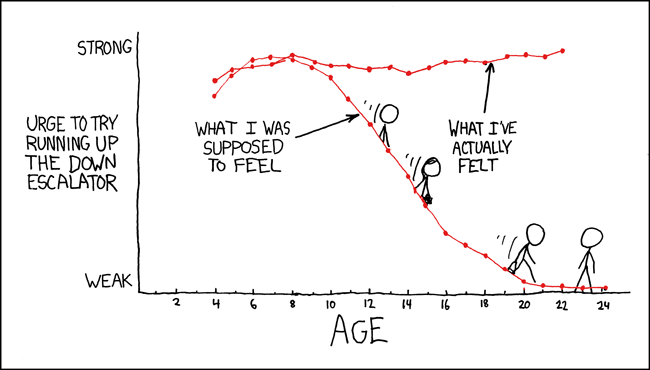
\includegraphics[width=.45\textwidth]{figures/escalators.png}}
  \end{figure}

When you print tables, it's good style to highlight the best results in bold. Also use the \textsc{booktabs} package for nicely formatted tables, as explained in the previous section on \LaTeX{} advice. (That's not a must, but it will simply look much nicer!)                    % evaluation
% \chapter{Concluding Remarks}\label{chap:conclusion}

If you wish, you may also name that section \emph{``Conclusion and Future Work''}, though it might not be a perfect choice to have a section named ``A \& B'' if it has subsections ``A'' and ``B''. Also note that you don't necessarily have to use these subsections; that also depends on how much content you have in each. (E.g., having a section header might be odd if it contains just three lines.)


\section{Conclusion}

This section usually summarizes the entire paper including the conclusions drawn, e.g., did the developed techniques work? Maybe add why or why not. Also don't hold back on limitations of your work; it shows that you understood what you have done. And science isn't about claiming how great something is, but about objectively testing hypotheses. Also note that every single scientific paper has such a section, so you can check out many examples, preferably at top-tier venues, e.g., by your supervisor(s).


\section{Future Work}

On top of that, you could discuss future work (and make clear why that is future work, i.e., by which observations did they get justified?).

Note that future work in scientific papers is often not mentioned at all or just in a very few sentences within the conclusion. That should not stop you from putting some effort in. This will (also) show the examiner(s)/supervisor(s) how well you understood the topic or how engaged you are.
                    % conclusion

% \appendix
% \chapter{Appendix: Explanation on Appendices}\label{chap:appendix1}

You may use appendices to provide additional information that is in principle relevant to your work, though you don't want \emph{every reader} to look at the entire material, but only those interested.

There are many cases where an appendix may make sense. For example:
\begin{itemize}
  \item You developed various variants of some algorithm, but you only describe one of them in the main body, since the different variants are not that different.
  \item You may have conducted an extensive empirical analysis, yet you don't want to provide \emph{all} results. So you focus on the most relevant results in the main body of your work to get the message across. Yet you present the remaining and complete results here for the more interested reader.
  \item You developed a model of some sort. In your work, you explained an excerpt of the model. You also used mathematical syntax for this. Here, you can (if you wish) provide the actual model as you provided it in probably some textfile. Note that you don't have to do this, as artifacts can be submitted separately. Consult your supervisor in such a case.
  \item You could also provide a list of figures and/or list of tables in here (via the commands \verb!\listoffigures! and \verb!\listoftables!, respectively). Do this only if you think that this is beneficial for your work. If you want to include it, you can of course also provide it right after the table of contents. You might want to make this dependent on how many people you think are interested in this.
\end{itemize}
                    % appendix 1
% \chapter{Appendix: Explanation on Page Borders}\label{chap:appendix2}

What you find here is an explanation of why the border width keeps flipping from left to right -- which you might have spotted and wondered why that's the case.

Firstly, that is \emph{intended} and thus correct, so there is no reason to worry about this. The reason is that this document is configured as a two-sided book, which means:
\begin{compactitem}
  \item We assume the document will be printed out,
  \item that this will be done in a two-sided mode (i.e., the document will be printed on both sides of each page), and
  \item that the bookbinding will be in the middle, just like in every book.
\end{compactitem}

When you open the book, there are three borders of equal size~$n$. This however requires that even pages have a border of $n$ on their left and $\frac{n}{2}$ on their right, and odd pages have a border of $\frac{n}{2}$ on their left and $n$ on their right. This is illustrated in Figure~\ref{fig:pageBorders}.

\begin{figure}[h]
  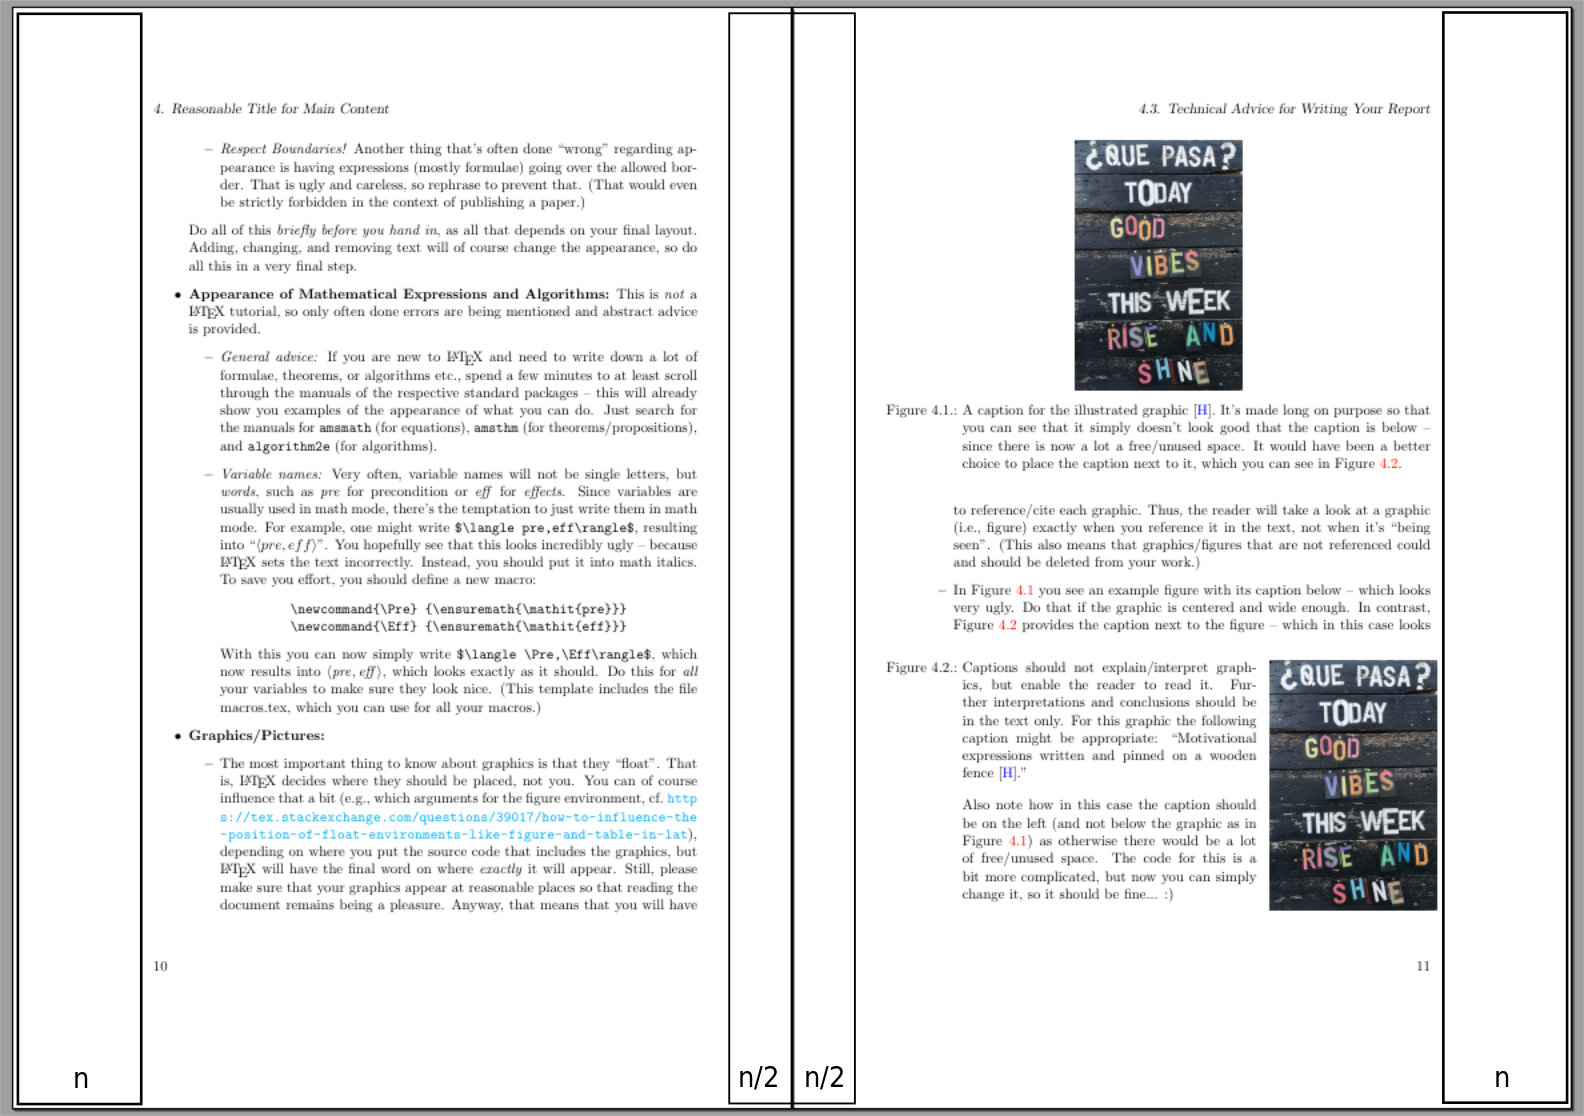
\includegraphics[width=.55\textwidth]{figures/borders--annotated}
  \caption{Illustration showing why page borders flip.\label{fig:pageBorders}}
\end{figure}%

                    % appendix 2


% literature
\bibliographystyle{unsrt} % or plainnat or whatever
\cleardoublepage\phantomsection
% see https://tex.stackexchange.com/questions/60556/link-to-bibliography-in-the-toc-fails
\bibliography{bib}
\end{document}
